% Options for packages loaded elsewhere
\PassOptionsToPackage{unicode}{hyperref}
\PassOptionsToPackage{hyphens}{url}
%
\documentclass[
]{book}
\usepackage{amsmath,amssymb}
\usepackage{iftex}
\ifPDFTeX
  \usepackage[T1]{fontenc}
  \usepackage[utf8]{inputenc}
  \usepackage{textcomp} % provide euro and other symbols
\else % if luatex or xetex
  \usepackage{unicode-math} % this also loads fontspec
  \defaultfontfeatures{Scale=MatchLowercase}
  \defaultfontfeatures[\rmfamily]{Ligatures=TeX,Scale=1}
\fi
\usepackage{lmodern}
\ifPDFTeX\else
  % xetex/luatex font selection
\fi
% Use upquote if available, for straight quotes in verbatim environments
\IfFileExists{upquote.sty}{\usepackage{upquote}}{}
\IfFileExists{microtype.sty}{% use microtype if available
  \usepackage[]{microtype}
  \UseMicrotypeSet[protrusion]{basicmath} % disable protrusion for tt fonts
}{}
\makeatletter
\@ifundefined{KOMAClassName}{% if non-KOMA class
  \IfFileExists{parskip.sty}{%
    \usepackage{parskip}
  }{% else
    \setlength{\parindent}{0pt}
    \setlength{\parskip}{6pt plus 2pt minus 1pt}}
}{% if KOMA class
  \KOMAoptions{parskip=half}}
\makeatother
\usepackage{xcolor}
\usepackage{color}
\usepackage{fancyvrb}
\newcommand{\VerbBar}{|}
\newcommand{\VERB}{\Verb[commandchars=\\\{\}]}
\DefineVerbatimEnvironment{Highlighting}{Verbatim}{commandchars=\\\{\}}
% Add ',fontsize=\small' for more characters per line
\usepackage{framed}
\definecolor{shadecolor}{RGB}{248,248,248}
\newenvironment{Shaded}{\begin{snugshade}}{\end{snugshade}}
\newcommand{\AlertTok}[1]{\textcolor[rgb]{0.94,0.16,0.16}{#1}}
\newcommand{\AnnotationTok}[1]{\textcolor[rgb]{0.56,0.35,0.01}{\textbf{\textit{#1}}}}
\newcommand{\AttributeTok}[1]{\textcolor[rgb]{0.13,0.29,0.53}{#1}}
\newcommand{\BaseNTok}[1]{\textcolor[rgb]{0.00,0.00,0.81}{#1}}
\newcommand{\BuiltInTok}[1]{#1}
\newcommand{\CharTok}[1]{\textcolor[rgb]{0.31,0.60,0.02}{#1}}
\newcommand{\CommentTok}[1]{\textcolor[rgb]{0.56,0.35,0.01}{\textit{#1}}}
\newcommand{\CommentVarTok}[1]{\textcolor[rgb]{0.56,0.35,0.01}{\textbf{\textit{#1}}}}
\newcommand{\ConstantTok}[1]{\textcolor[rgb]{0.56,0.35,0.01}{#1}}
\newcommand{\ControlFlowTok}[1]{\textcolor[rgb]{0.13,0.29,0.53}{\textbf{#1}}}
\newcommand{\DataTypeTok}[1]{\textcolor[rgb]{0.13,0.29,0.53}{#1}}
\newcommand{\DecValTok}[1]{\textcolor[rgb]{0.00,0.00,0.81}{#1}}
\newcommand{\DocumentationTok}[1]{\textcolor[rgb]{0.56,0.35,0.01}{\textbf{\textit{#1}}}}
\newcommand{\ErrorTok}[1]{\textcolor[rgb]{0.64,0.00,0.00}{\textbf{#1}}}
\newcommand{\ExtensionTok}[1]{#1}
\newcommand{\FloatTok}[1]{\textcolor[rgb]{0.00,0.00,0.81}{#1}}
\newcommand{\FunctionTok}[1]{\textcolor[rgb]{0.13,0.29,0.53}{\textbf{#1}}}
\newcommand{\ImportTok}[1]{#1}
\newcommand{\InformationTok}[1]{\textcolor[rgb]{0.56,0.35,0.01}{\textbf{\textit{#1}}}}
\newcommand{\KeywordTok}[1]{\textcolor[rgb]{0.13,0.29,0.53}{\textbf{#1}}}
\newcommand{\NormalTok}[1]{#1}
\newcommand{\OperatorTok}[1]{\textcolor[rgb]{0.81,0.36,0.00}{\textbf{#1}}}
\newcommand{\OtherTok}[1]{\textcolor[rgb]{0.56,0.35,0.01}{#1}}
\newcommand{\PreprocessorTok}[1]{\textcolor[rgb]{0.56,0.35,0.01}{\textit{#1}}}
\newcommand{\RegionMarkerTok}[1]{#1}
\newcommand{\SpecialCharTok}[1]{\textcolor[rgb]{0.81,0.36,0.00}{\textbf{#1}}}
\newcommand{\SpecialStringTok}[1]{\textcolor[rgb]{0.31,0.60,0.02}{#1}}
\newcommand{\StringTok}[1]{\textcolor[rgb]{0.31,0.60,0.02}{#1}}
\newcommand{\VariableTok}[1]{\textcolor[rgb]{0.00,0.00,0.00}{#1}}
\newcommand{\VerbatimStringTok}[1]{\textcolor[rgb]{0.31,0.60,0.02}{#1}}
\newcommand{\WarningTok}[1]{\textcolor[rgb]{0.56,0.35,0.01}{\textbf{\textit{#1}}}}
\usepackage{longtable,booktabs,array}
\usepackage{calc} % for calculating minipage widths
% Correct order of tables after \paragraph or \subparagraph
\usepackage{etoolbox}
\makeatletter
\patchcmd\longtable{\par}{\if@noskipsec\mbox{}\fi\par}{}{}
\makeatother
% Allow footnotes in longtable head/foot
\IfFileExists{footnotehyper.sty}{\usepackage{footnotehyper}}{\usepackage{footnote}}
\makesavenoteenv{longtable}
\usepackage{graphicx}
\makeatletter
\newsavebox\pandoc@box
\newcommand*\pandocbounded[1]{% scales image to fit in text height/width
  \sbox\pandoc@box{#1}%
  \Gscale@div\@tempa{\textheight}{\dimexpr\ht\pandoc@box+\dp\pandoc@box\relax}%
  \Gscale@div\@tempb{\linewidth}{\wd\pandoc@box}%
  \ifdim\@tempb\p@<\@tempa\p@\let\@tempa\@tempb\fi% select the smaller of both
  \ifdim\@tempa\p@<\p@\scalebox{\@tempa}{\usebox\pandoc@box}%
  \else\usebox{\pandoc@box}%
  \fi%
}
% Set default figure placement to htbp
\def\fps@figure{htbp}
\makeatother
\setlength{\emergencystretch}{3em} % prevent overfull lines
\providecommand{\tightlist}{%
  \setlength{\itemsep}{0pt}\setlength{\parskip}{0pt}}
\setcounter{secnumdepth}{5}
\usepackage{booktabs}
\usepackage[]{natbib}
\bibliographystyle{plainnat}
\usepackage{bookmark}
\IfFileExists{xurl.sty}{\usepackage{xurl}}{} % add URL line breaks if available
\urlstyle{same}
\hypersetup{
  pdftitle={UCSCXenaShiny v2 Book},
  pdfauthor={Shensuo Li, Shixiang Wang},
  hidelinks,
  pdfcreator={LaTeX via pandoc}}

\title{UCSCXenaShiny v2 Book}
\author{Shensuo Li, Shixiang Wang}
\date{2025-08-09}

\begin{document}
\maketitle

{
\setcounter{tocdepth}{1}
\tableofcontents
}
\chapter*{About}\label{about}
\addcontentsline{toc}{chapter}{About}

\textbf{UCSCXenaShiny} is an R package for interactively exploring UCSC Xena datasets. It is mainly designed to provide a web app (built on the top of \href{https://shiny.rstudio.com/}{\texttt{\{shiny\}}} framework and \href{https://github.com/ropensci/UCSCXenaTools/}{\texttt{\{UCSCXenaTools\}}} package) for downloading, analyzing and visualizing datasets from \href{https://xenabrowser.net/datapages/}{UCSC Xena}. In the latest version, the application can support both general and personalized tumor molecular analysis with versatile functional modules and user-friendly interface layouts. Overall, our tool aims to make best use of public omics data from UCSC Xena and assist broad user community with precision oncology research.

\begin{center}\includegraphics[width=1\linewidth]{images/p0000_1} \end{center}

Here, we have prepared the tutorial book to introduce the detailed usage of UCSCXenaShiny based on R Markdown and \href{https://github.com/rstudio/bookdown}{bookdown}. Firstly, we will start with the basic knowledge of UCSC Xena repository and its data hubs in \textbf{Chapter \ref{intro}}. Then, the following chapters can be generally divided into two parts for the usage of R package and Shiny App:

\subsubsection*{Part Ⅰ}\label{part-ux2170}
\addcontentsline{toc}{subsubsection}{Part Ⅰ}

\begin{itemize}
\tightlist
\item
  \textbf{Chapter \ref{install}}：The ways to install UCSCXenaShiny package.
\item
  \textbf{Chapter \ref{build-in}}：Avalilable built-in datasets of package, e.g.~clinical or survival data.
\item
  \textbf{Chapter \ref{data-query}}：The functions to query molecular data of TPC datasets.
\item
  \textbf{Chapter \ref{data-analysis}}：The functions to perform various analyses based on TPC datasets.
\end{itemize}

\subsubsection*{Part Ⅱ}\label{part-ux2171}
\addcontentsline{toc}{subsubsection}{Part Ⅱ}

\begin{itemize}
\tightlist
\item
  \textbf{Chapter \ref{visit}}：The ways to visit UCSCXenaShiny application.
\item
  \textbf{Chapter \ref{home}}：The intuitive widgets and quick exploration modules in homepage.
\item
  \textbf{Chapter \ref{repo}}：The query for all datasets of UCSC Xena repository.
\item
  \textbf{Chapter \ref{general-da}}：General analysis modules for any matrix datasets.
\item
  \textbf{Chapter \ref{custom-tpc}}：Custom analysis modules for TPC datasets.
\item
  \textbf{Chapter \ref{per-tpc-1}}：The key preprocesses of personalized TPC pipelines.
\item
  \textbf{Chapter \ref{per-tpc-2}}：The versatile analyses of personalized TPC pipelines.
\item
  \textbf{Chapter \ref{download}}：Two download modules for the custom data subset.
\end{itemize}

\subsubsection*{Part Ⅲ}\label{part-ux2172}
\addcontentsline{toc}{subsubsection}{Part Ⅲ}

We have recorded a series of tutorial videos with step-by-step instructions:

\textbf{1. English version}

\begin{itemize}
\tightlist
\item
  Episode 1-4: \url{https://www.youtube.com/watch?v=VnIlzcVB1Ow&list=PLN1jxcOQONG6pH8zvHr-qhI3MMtvluITf}
\end{itemize}

\begin{center}\includegraphics[width=0.9\linewidth]{images/p0000_2} \end{center}

\textbf{2. Chinese version}

\begin{itemize}
\tightlist
\item
  Episode 1: \url{https://www.bilibili.com/video/BV1rT421k7Zv}
\item
  Episode 2: \url{https://www.bilibili.com/video/BV1E14218779}
\item
  Episode 3: \url{https://www.bilibili.com/video/BV141421t71g}
\item
  Episode 4: \url{https://www.bilibili.com/video/BV1TZ421K7VH}
\end{itemize}

\begin{center}\rule{0.5\linewidth}{0.5pt}\end{center}

Welcome to cite the following articles when \textbf{UCSCXenaShiny} has facilitated your study:

\begin{enumerate}
\def\labelenumi{\arabic{enumi}.}
\item
  \textbf{UCSCXenaShiny} \textbf{v2} ---

  Li, S., Peng, Y., Chen, M. \emph{et al.} Facilitating integrative and personalized oncology omics analysis with UCSCXenaShiny. \emph{Commun Biol} \textbf{7}, 1200 (2024). \url{https://doi.org/10.1038/s42003-024-06891-2}
\item
  \textbf{UCSCXenaShiny} \textbf{v1} ---

  Shixiang Wang, Yi Xiong, Longfei Zhao, Kai Gu, Yin Li, Fei Zhao, Jianfeng Li, Mingjie Wang, Haitao Wang, Ziyu Tao, Tao Wu, Yichao Zheng, Xuejun Li, Xue-Song Liu, UCSCXenaShiny: an R/CRAN package for interactive analysis of UCSC Xena data, \emph{Bioinformatics}, Volume 38, Issue 2, January 2022, Pages 527--529, \url{https://doi.org/10.1093/bioinformatics/btab561}
\item
  \textbf{UCSCXenaTools} ---

  Wang S and Liu X. The UCSCXenaTools R package: a toolkit for accessing genomics data from UCSC Xena platform, from cancer multi-omics to single-cell RNA-seq. Journal of Open Source Software, 4(40), 1627, \url{https://doi.org/10.21105/joss.01627}
\end{enumerate}

\begin{quote}
If you have any question, please report to the \href{https://github.com/openbiox/UCSCXenaShiny/issues}{Github issues page} or email to \href{mailto:lishensuo@163.com}{\nolinkurl{lishensuo@163.com}}
\end{quote}

\chapter{Introduction}\label{intro}

\section{UCSC Xena Datasets}\label{ucsc-xena-datasets}

\href{https://xenabrowser.net/datapages/}{UCSC Xena platform} is developed by the UC Santa Cruz Genomics Institute and serves as a comprehensive repository to provide thousands of processed omics datasets from large cancer research projects (e.g.~TCGA, PCAWG and CCLE) or individual research groups and enable unprecedented research opportunities.

The hierarchy for storing and querying datasets is as follows:

\begin{itemize}
\tightlist
\item
  The UCSC Xena repository is generally comprised of \textbf{11} data hubs from various portals;
\item
  Each data hub could include many sample cohorts;
\item
  Each sample cohort could involve multiple omics profiling or phenotype data;
\item
  Each omics profiling could have several datasets due to normalization methods or other factors.
\end{itemize}

\begin{figure}

{\centering \includegraphics[width=0.8\linewidth]{images/p0201} 

}

\caption{The hierarchy of datasets in UCSC Xena}\label{fig:p0201}
\end{figure}

\begin{quote}
Note: In the UCSCXenaShiny, we summarized all the data (sub)types into four main types, referring to \emph{clinicalMatrix}, \emph{genomicsMatrix}, \emph{genomicSegment}, \emph{mutationVector}, where the genomicsMatrix is the key component.
\end{quote}

\begin{figure}

{\centering \includegraphics[width=0.8\linewidth]{images/p0202} 

}

\caption{The main types and subtypes of datasets}\label{fig:p0202}
\end{figure}

The following figure shows the numbers of cohorts and datasets for each datahub of UCSC Xena. Although some hubs (like toilHub, pancanAtlasHub) have relatively lower numbers of datasets, they mainly focus of pan-cancer integration, which could be more valuable in some research. Here, we will briefly introduce these hubs for better use.

\begin{figure}

{\centering \includegraphics[width=0.8\linewidth]{images/p0203} 

}

\caption{The statitics for cohorts and datasets of each data hub}\label{fig:p0203}
\end{figure}

\subsubsection*{\texorpdfstring{(1) \href{https://xenabrowser.net/datapages/?host=https\%3A\%2F\%2Ftcga.xenahubs.net&removeHub=https\%3A\%2F\%2Fxena.treehouse.gi.ucsc.edu\%3A443}{tcgaHub (TCGA hub)}}{(1) tcgaHub (TCGA hub)}}\label{tcgahub-tcga-hub}
\addcontentsline{toc}{subsubsection}{(1) \href{https://xenabrowser.net/datapages/?host=https\%3A\%2F\%2Ftcga.xenahubs.net&removeHub=https\%3A\%2F\%2Fxena.treehouse.gi.ucsc.edu\%3A443}{tcgaHub (TCGA hub)}}

\begin{itemize}
\tightlist
\item
  \textbf{Statistics}: 38 cohorts, 715 datasets;
\item
  \textbf{Source}: TCGA Data Coordinating Center (\href{https://www.cancer.gov/ccg/research/genome-sequencing/tcga}{DCC}), Jan 2016
\item
  \textbf{Description}: The hub is specific to the \href{https://www.cancer.gov/ccg/research/genome-sequencing/tcga}{TCGA project} with both individual tumor or integrative pan-cancer cohorts
\end{itemize}

\subsubsection*{\texorpdfstring{(2) \href{https://xenabrowser.net/datapages/?host=https\%3A\%2F\%2Fgdc.xenahubs.net&removeHub=https\%3A\%2F\%2Fxena.treehouse.gi.ucsc.edu\%3A443}{gdcHub (GDC hub)}}{(2) gdcHub (GDC hub)}}\label{gdchub-gdc-hub}
\addcontentsline{toc}{subsubsection}{(2) \href{https://xenabrowser.net/datapages/?host=https\%3A\%2F\%2Fgdc.xenahubs.net&removeHub=https\%3A\%2F\%2Fxena.treehouse.gi.ucsc.edu\%3A443}{gdcHub (GDC hub)}}

\begin{itemize}
\tightlist
\item
  \textbf{Statistics}: 42 cohorts, 534 datasets;
\item
  \textbf{Source}: GDC Data Portal (\href{https://portal.gdc.cancer.gov/}{GDC}), v18.0, 2019-08-28
\item
  \textbf{Description}: The hub incorporates TCGA project with both individual tumor or integrative pan-cancer cohorts, as well as \href{https://www.cancer.gov/ccg/research/genome-sequencing/target}{TARGET project} (childhood cancers).
\end{itemize}

\subsubsection*{\texorpdfstring{(3) \href{https://xenabrowser.net/datapages/?host=https\%3A\%2F\%2Fpancanatlas.xenahubs.net&removeHub=https\%3A\%2F\%2Fxena.treehouse.gi.ucsc.edu\%3A443}{pancanAtlasHub (Pan-Cancer Atlas Hub)}}{(3) pancanAtlasHub (Pan-Cancer Atlas Hub)}}\label{pancanatlashub-pan-cancer-atlas-hub}
\addcontentsline{toc}{subsubsection}{(3) \href{https://xenabrowser.net/datapages/?host=https\%3A\%2F\%2Fpancanatlas.xenahubs.net&removeHub=https\%3A\%2F\%2Fxena.treehouse.gi.ucsc.edu\%3A443}{pancanAtlasHub (Pan-Cancer Atlas Hub)}}

\begin{itemize}
\tightlist
\item
  \textbf{Statistics}: 1 cohort, 22 datasets;
\item
  \textbf{Source}: \href{http://www.cell.com/pb-assets/consortium/PanCancerAtlas/PanCani3/index.html}{Pan-Cancer Atlas publications on Cell}.
\item
  \textbf{Description}: The hub collects the curated pan-cancer TCGA data generated by the PanCan Atlas consortium working groups.
\end{itemize}

\subsubsection*{\texorpdfstring{(4) \href{https://xenabrowser.net/datapages/?host=https\%3A\%2F\%2Ftoil.xenahubs.net&removeHub=https\%3A\%2F\%2Fxena.treehouse.gi.ucsc.edu\%3A443}{toilHub (UCSC Toil RNA-seq Recompute)}}{(4) toilHub (UCSC Toil RNA-seq Recompute)}}\label{toilhub-ucsc-toil-rna-seq-recompute}
\addcontentsline{toc}{subsubsection}{(4) \href{https://xenabrowser.net/datapages/?host=https\%3A\%2F\%2Ftoil.xenahubs.net&removeHub=https\%3A\%2F\%2Fxena.treehouse.gi.ucsc.edu\%3A443}{toilHub (UCSC Toil RNA-seq Recompute)}}

\begin{itemize}
\tightlist
\item
  \textbf{Statistics}: 5 cohort, 51 datasets;
\item
  \textbf{Source}: \href{https://www.nature.com/articles/nbt.3772}{The toil pipleline from UCSC Genomics Institute}.
\item
  \textbf{Description}: The hub aims to integrate the pan-cancer RNA-seq data from TCGA, TARGET and \href{https://gtexportal.org/home/}{GTEx} databases.
\end{itemize}

\subsubsection*{\texorpdfstring{(5) \href{https://xenabrowser.net/datapages/?host=https\%3A\%2F\%2Fucscpublic.xenahubs.net&removeHub=https\%3A\%2F\%2Fxena.treehouse.gi.ucsc.edu\%3A443}{publicHub (UCSC Public Hub)}}{(5) publicHub (UCSC Public Hub)}}\label{publichub-ucsc-public-hub}
\addcontentsline{toc}{subsubsection}{(5) \href{https://xenabrowser.net/datapages/?host=https\%3A\%2F\%2Fucscpublic.xenahubs.net&removeHub=https\%3A\%2F\%2Fxena.treehouse.gi.ucsc.edu\%3A443}{publicHub (UCSC Public Hub)}}

\begin{itemize}
\tightlist
\item
  \textbf{Statistics}: 37 cohort, 114 datasets;
\item
  \textbf{Source}: Public resources from extensive collection.
\item
  \textbf{Description}: The hub collects various cancer (or cell lines, e.g.~CCLE, CMAP) omics data from other public studies.
\end{itemize}

\subsubsection*{\texorpdfstring{(6) \href{https://xenabrowser.net/datapages/?host=https\%3A\%2F\%2Ficgc.xenahubs.net&removeHub=https\%3A\%2F\%2Fxena.treehouse.gi.ucsc.edu\%3A443}{icgcHub (ICGC Xena Hub)}}{(6) icgcHub (ICGC Xena Hub)}}\label{icgchub-icgc-xena-hub}
\addcontentsline{toc}{subsubsection}{(6) \href{https://xenabrowser.net/datapages/?host=https\%3A\%2F\%2Ficgc.xenahubs.net&removeHub=https\%3A\%2F\%2Fxena.treehouse.gi.ucsc.edu\%3A443}{icgcHub (ICGC Xena Hub)}}

\begin{itemize}
\tightlist
\item
  \textbf{Statistics}: 3 cohort, 23 datasets;
\item
  \textbf{Source}: \href{https://dcc.icgc.org/}{International Cancer Genome Consortium(ICGC)}.
\item
  \textbf{Description}: The hub considers the genomics data from ICGC but only included the US(TCGA) related projects for Gene/Protein expression data.
\end{itemize}

\subsubsection*{\texorpdfstring{(7) \href{https://xenabrowser.net/datapages/?host=https\%3A\%2F\%2Fpcawg.xenahubs.net&removeHub=https\%3A\%2F\%2Fxena.treehouse.gi.ucsc.edu\%3A443}{pcawgHub (PCAWG Hub)}}{(7) pcawgHub (PCAWG Hub)}}\label{pcawghub-pcawg-hub}
\addcontentsline{toc}{subsubsection}{(7) \href{https://xenabrowser.net/datapages/?host=https\%3A\%2F\%2Fpcawg.xenahubs.net&removeHub=https\%3A\%2F\%2Fxena.treehouse.gi.ucsc.edu\%3A443}{pcawgHub (PCAWG Hub)}}

\begin{itemize}
\tightlist
\item
  \textbf{Statistics}: 2 cohort, 53 datasets;
\item
  \textbf{Source}: \href{https://xenabrowser.net/datapages/?host=https\%3A\%2F\%2Fpcawg.xenahubs.net&removeHub=https\%3A\%2F\%2Fxena.treehouse.gi.ucsc.edu\%3A443}{The Pancancer Analysis of Whole Genomes (PCAWG) study}.
\item
  \textbf{Description}: The hub focus on multi-omics data of cancer whole genomes across many tumor types from \href{https://dcc.icgc.org/}{International Cancer Genome Consortium(ICGC)}.
\end{itemize}

\subsubsection*{\texorpdfstring{(8) \href{https://xenabrowser.net/datapages/?host=https\%3A\%2F\%2Fatacseq.xenahubs.net}{atacseqHub(ATAC-seq Hub)}}{(8) atacseqHub(ATAC-seq Hub)}}\label{atacseqhubatac-seq-hub}
\addcontentsline{toc}{subsubsection}{(8) \href{https://xenabrowser.net/datapages/?host=https\%3A\%2F\%2Fatacseq.xenahubs.net}{atacseqHub(ATAC-seq Hub)}}

\begin{itemize}
\tightlist
\item
  \textbf{Statistics}: 2 cohort, 9 datasets;
\item
  \textbf{Source}: \href{https://www.science.org/doi/10.1126/science.aav1898}{The chromatin accessibility landscape of primary human cancers}
\item
  \textbf{Description}: The hub describes chromatin accessibility of 410 TCGA tumor samples across 23 cancer types using the ATAC-seq technology.
\end{itemize}

\subsubsection*{\texorpdfstring{(9) \href{https://xenabrowser.net/datapages/?host=https\%3A\%2F\%2Fkidsfirst.xenahubs.net&removeHub=https\%3A\%2F\%2Fxena.treehouse.gi.ucsc.edu\%3A443}{kidfirstHub(Kids First Xena Hub)}}{(9) kidfirstHub(Kids First Xena Hub)}}\label{kidfirsthubkids-first-xena-hub}
\addcontentsline{toc}{subsubsection}{(9) \href{https://xenabrowser.net/datapages/?host=https\%3A\%2F\%2Fkidsfirst.xenahubs.net&removeHub=https\%3A\%2F\%2Fxena.treehouse.gi.ucsc.edu\%3A443}{kidfirstHub(Kids First Xena Hub)}}

\begin{itemize}
\tightlist
\item
  \textbf{Statistics}: 3 cohort, 50 datasets;
\item
  \textbf{Source}: \href{https://portal.kidsfirstdrc.org/}{the Gabriella Miller Kids First Pediatric Research Program}
\item
  \textbf{Description}: The hub incorporates Pediatric Brain Tumor Atlas and TARGET project.
\end{itemize}

\subsubsection*{\texorpdfstring{(10) \href{https://xenabrowser.net/datapages/?host=https\%3A\%2F\%2Fxena.treehouse.gi.ucsc.edu\%3A443&removeHub=https\%3A\%2F\%2Fxena.treehouse.gi.ucsc.edu\%3A443}{treehouseHub}}{(10) treehouseHub}}\label{treehousehub}
\addcontentsline{toc}{subsubsection}{(10) \href{https://xenabrowser.net/datapages/?host=https\%3A\%2F\%2Fxena.treehouse.gi.ucsc.edu\%3A443&removeHub=https\%3A\%2F\%2Fxena.treehouse.gi.ucsc.edu\%3A443}{treehouseHub}}

\begin{itemize}
\tightlist
\item
  \textbf{Statistics}: 16 cohorts, 44 datasets
\item
  \textbf{Source}: \href{https://treehousegenomics.soe.ucsc.edu/public-data/}{the Treehouse Childhood Cancer Initiative}
\item
  \textbf{Description}: The hub is also specific to children cancer.
\end{itemize}

\subsubsection*{\texorpdfstring{(11) \href{https://singlecellnew.xenahubs.net}{singlecellHub}}{(11) singlecellHub}}\label{singlecellhub}
\addcontentsline{toc}{subsubsection}{(11) \href{https://singlecellnew.xenahubs.net}{singlecellHub}}

\begin{itemize}
\tightlist
\item
  \textbf{Statistics}: 16 cohorts, 71 datasets
\item
  \textbf{Source}: \href{https://data.humancellatlas.org/}{Human Cell Atlas (HCA)}
\item
  \textbf{Description}: The hub includes several scRNA-seq datasets from HCA, invovling cancer or normal tissues, human or mouse origin.
\end{itemize}

\section{TCGA abbreviations}\label{tcga-abbreviations}

\begin{table}

\caption{\label{tab:tb04-1}TCGA abbreviations}
\centering
\begin{tabular}[t]{lll}
\toprule
 & Abbreviation & Name\\
\midrule
1 & LAML & Acute Myeloid Leukemia\\
2 & ACC & Adrenocortical carcinoma\\
3 & BLCA & Bladder Urothelial Carcinoma\\
4 & LGG & Brain Lower Grade Glioma\\
5 & BRCA & Breast invasive carcinoma\\
\addlinespace
6 & CESC & Cervical squamous cell carcinoma and endocervical adenocarcinoma\\
7 & CHOL & Cholangiocarcinoma\\
8 & LCML & Chronic Myelogenous Leukemia\\
9 & COAD & Colon adenocarcinoma\\
10 & CNTL & Controls\\
\addlinespace
11 & ESCA & Esophageal carcinoma\\
12 & FPPP & FFPE Pilot Phase II\\
13 & GBM & Glioblastoma multiforme\\
14 & HNSC & Head and Neck squamous cell carcinoma\\
15 & KICH & Kidney Chromophobe\\
\addlinespace
16 & KIRC & Kidney renal clear cell carcinoma\\
17 & KIRP & Kidney renal papillary cell carcinoma\\
18 & LIHC & Liver hepatocellular carcinoma\\
19 & LUAD & Lung adenocarcinoma\\
20 & LUSC & Lung squamous cell carcinoma\\
\addlinespace
21 & DLBC & Lymphoid Neoplasm Diffuse Large B-cell Lymphoma\\
22 & MESO & Mesothelioma\\
23 & MISC & Miscellaneous\\
24 & OV & Ovarian serous cystadenocarcinoma\\
25 & PAAD & Pancreatic adenocarcinoma\\
\addlinespace
26 & PCPG & Pheochromocytoma and Paraganglioma\\
27 & PRAD & Prostate adenocarcinoma\\
28 & READ & Rectum adenocarcinoma\\
29 & SARC & Sarcoma\\
30 & SKCM & Skin Cutaneous Melanoma\\
\addlinespace
31 & STAD & Stomach adenocarcinoma\\
32 & TGCT & Testicular Germ Cell Tumors\\
33 & THYM & Thymoma\\
34 & THCA & Thyroid carcinoma\\
35 & UCS & Uterine Carcinosarcoma\\
\addlinespace
36 & UCEC & Uterine Corpus Endometrial Carcinoma\\
37 & UVM & Uveal Melanoma\\
\bottomrule
\end{tabular}
\end{table}

\section{PCAWG abbreviations}\label{pcawg-abbreviations}

\begin{table}

\caption{\label{tab:tb04-2}PCAWG abbreviations}
\centering
\begin{tabular}[t]{lll}
\toprule
 & Abbreviation & Name\\
\midrule
1 & BLCA-US & Bladder Urothelial Cancer - TCGA, US\\
2 & BRCA-US & Breast Cancer - TCGA, US\\
3 & CESC-US & Cervical Squamous Cell Carcinoma - TCGA, US\\
4 & CLLE-ES & Chronic Lymphocytic Leukemia - ES\\
5 & COAD-US & Colon Adenocarcinoma - TCGA, US\\
\addlinespace
6 & DLBC-US & Lymphoid Neoplasm Diffuse Large B-cell Lymphoma - TCGA, US\\
7 & ESAD-UK & Esophageal Adenocarcinoma - UK\\
8 & GBM-US & Brain Glioblastoma Multiforme - TCGA, US\\
9 & HNSC-US & Head and Neck Squamous Cell Carcinoma - TCGA, US\\
10 & KICH-US & Kidney Chromophobe - TCGA, US\\
\addlinespace
11 & KIRC-US & Kidney Renal Clear Cell Carcinoma - TCGA, US\\
12 & KIRP-US & Kidney Renal Papillary Cell Carcinoma - TCGA, US\\
13 & LAML-US & Acute Myeloid Leukemia - TCGA, US\\
14 & LGG-US & Brain Lower Grade Glioma - TCGA, US\\
15 & LIHC-US & Liver Hepatocellular carcinoma - TCGA, US\\
\addlinespace
16 & LIRI-JP & Liver Cancer - RIKEN, JP\\
17 & LUAD-US & Lung Adenocarcinoma - TCGA, US\\
18 & LUSC-US & Lung Squamous Cell Carcinoma - TCGA, US\\
19 & MALY-DE & Malignant Lymphoma - DE\\
20 & OV-AU & Ovarian Cancer - AU\\
\addlinespace
21 & OV-US & Ovarian Serous Cystadenocarcinoma - TCGA, US\\
22 & PACA-AU & Pancreatic Cancer - AU\\
23 & PRAD-US & Prostate Adenocarcinoma - TCGA, US\\
24 & READ-US & Rectum Adenocarcinoma - TCGA, US\\
25 & RECA-EU & Renal Cell Cancer - EU/FR\\
\addlinespace
26 & SARC-US & Sarcoma - TCGA, US\\
27 & SKCM-US & Skin Cutaneous melanoma - TCGA, US\\
28 & STAD-US & Gastric Adenocarcinoma - TCGA, US\\
29 & THCA-US & Head and Neck Thyroid Carcinoma - TCGA, US\\
30 & UCEC-US & Uterine Corpus Endometrial Carcinoma- TCGA, US\\
\bottomrule
\end{tabular}
\end{table}

\part{R Package}\label{part-r-package}

\chapter{Install}\label{install}

Here, we have provided several ways to install UCSCXenaShiny R package. You can see the detailed instruction and troubleshooting information from the README file of our \href{https://github.com/openbiox/UCSCXenaShiny}{Github project}.

\section{CRAN}\label{cran}

\begin{itemize}
\tightlist
\item
  \url{https://cran.r-project.org/package=UCSCXenaShiny}
\end{itemize}

\begin{Shaded}
\begin{Highlighting}[]
\CommentTok{\# Online}
\FunctionTok{install.packages}\NormalTok{(}\StringTok{"UCSCXenaShiny"}\NormalTok{)}
\DocumentationTok{\#\# or specific repos}
\FunctionTok{install.packages}\NormalTok{(}\StringTok{"UCSCXenaShiny"}\NormalTok{, }\AttributeTok{repos =} \FunctionTok{c}\NormalTok{(}\StringTok{"https://openbiox.r{-}universe.dev"}\NormalTok{, }\StringTok{"https://cran.r{-}project.org"}\NormalTok{))}

\CommentTok{\# Local}
\FunctionTok{install.packages}\NormalTok{(}\StringTok{"UCSCXenaShiny\_2.0.0.tar.gz"}\NormalTok{, }\AttributeTok{repos =} \ConstantTok{NULL}\NormalTok{, }\AttributeTok{type=}\StringTok{"source"}\NormalTok{)}
\end{Highlighting}
\end{Shaded}

\begin{itemize}
\tightlist
\item
  Once the package has been installed successfully, your can load it and check its version:
\end{itemize}

\begin{Shaded}
\begin{Highlighting}[]
\FunctionTok{library}\NormalTok{(UCSCXenaShiny)}
\end{Highlighting}
\end{Shaded}

\begin{verbatim}
## =========================================================================================
## UCSCXenaShiny version 2.2.0
## Project URL: https://github.com/openbiox/UCSCXenaShiny
## Usages: https://openbiox.github.io/UCSCXenaShiny/
## 
## If you use it in published research, please cite:
##   Shensuo Li, Yuzhong Peng, Minjun Chen, Yankun Zhao, Yi Xiong, Jianfeng Li, Peng Luo, 
##   Haitao Wang, Fei Zhao, Qi Zhao, Yanru Cui, Sujun Chen, Jian-Guo Zhou, Shixiang Wang,  
##   Facilitating integrative and personalized oncology omics analysis with UCSCXenaShiny, 
##   Communications Biology, 1200 (2024),  https://doi.org/10.1038/s42003-024-06891-2
## =========================================================================================
##                               --Enjoy it--
\end{verbatim}

\begin{Shaded}
\begin{Highlighting}[]
\FunctionTok{packageVersion}\NormalTok{(}\StringTok{"UCSCXenaShiny"}\NormalTok{)}
\end{Highlighting}
\end{Shaded}

\begin{verbatim}
## [1] '2.2.0'
\end{verbatim}

\section{Github}\label{github}

\begin{Shaded}
\begin{Highlighting}[]
\CommentTok{\# Online}
\NormalTok{devtools}\SpecialCharTok{::}\FunctionTok{install\_github}\NormalTok{(}\StringTok{"openbiox/UCSCXenaShiny"}\NormalTok{)}

\CommentTok{\# Local}
\NormalTok{devtools}\SpecialCharTok{::}\FunctionTok{install\_local}\NormalTok{(}\AttributeTok{path =} \StringTok{"UCSCXenaShiny{-}master.zip"}\NormalTok{)}
\end{Highlighting}
\end{Shaded}

\section{Conda}\label{conda}

\begin{Shaded}
\begin{Highlighting}[]
\ExtensionTok{conda}\NormalTok{ install }\AttributeTok{{-}c}\NormalTok{ conda{-}forge r{-}ucscxenashiny}
\end{Highlighting}
\end{Shaded}

\begin{itemize}
\tightlist
\item
  list all of the versions of r-ucscxenashiny available on your platform:
\end{itemize}

\begin{Shaded}
\begin{Highlighting}[]
\ExtensionTok{conda}\NormalTok{ search r{-}ucscxenashiny }\AttributeTok{{-}{-}channel}\NormalTok{ conda{-}forge}
\end{Highlighting}
\end{Shaded}

\section{Docker}\label{docker}

\begin{Shaded}
\begin{Highlighting}[]
\CommentTok{\# install image}
\ExtensionTok{docker}\NormalTok{ pull shixiangwang/ucscxenashiny}

\CommentTok{\# run image}
\ExtensionTok{docker}\NormalTok{ run }\AttributeTok{{-}d} \AttributeTok{{-}{-}name}\NormalTok{ xenashiny }\AttributeTok{{-}p}\NormalTok{ 3838:3838 shixiangwang/ucscxenashiny}
\end{Highlighting}
\end{Shaded}

\chapter{Built-in Datasets}\label{build-in}

We also have curated tens of tumor non-omics annotation datasets with supplementary features from UCSC Xena repository or other resources for extensive analysis. Notably, datasets with large amounts of data are uploaded to Zenodo. They can be loaded via \texttt{load\_data()} function.

\begin{figure}

{\centering \includegraphics[width=0.8\linewidth]{images/p001} 

}

\caption{UCSCXenaShiny built-in datasets}\label{fig:builtin-datasets}
\end{figure}

\section{TCGA}\label{tcga}

\begin{itemize}
\tightlist
\item
  \texttt{TCGA.organ}: Detailed information of 33 TCGA projects
\end{itemize}

\begin{Shaded}
\begin{Highlighting}[]
\FunctionTok{head}\NormalTok{(TCGA.organ)}
\end{Highlighting}
\end{Shaded}

\begin{verbatim}
##   TCGA                              Detail    organ
## 1 BRCA           breast invasive carcinoma   breast
## 2 PRAD             prostate adenocarcinoma prostate
## 3   OV   ovarian serous cystadenocarcinoma    ovary
## 4 PCPG    pheochromocytoma & paraganglioma         
## 5  GBM             glioblastoma multiforme    brain
## 6 HNSC head & neck squamous cell carcinoma
\end{verbatim}

\begin{itemize}
\tightlist
\item
  \texttt{tcga\_gtex}: Merged information of TCGA and GTEx samples
\end{itemize}

\begin{Shaded}
\begin{Highlighting}[]
\FunctionTok{head}\NormalTok{(tcga\_gtex)}
\end{Highlighting}
\end{Shaded}

\begin{verbatim}
##            sample tissue            type type2
## 1 TCGA-D3-A1QA-07   SKCM SKCM_tumor_TCGA tumor
## 2 TCGA-DE-A4MD-06   THCA THCA_tumor_TCGA tumor
## 3 TCGA-J8-A3O2-06   THCA THCA_tumor_TCGA tumor
## 4 TCGA-J8-A3YH-06   THCA THCA_tumor_TCGA tumor
## 5 TCGA-EM-A2P1-06   THCA THCA_tumor_TCGA tumor
## 6 TCGA-J8-A4HW-06   THCA THCA_tumor_TCGA tumor
\end{verbatim}

\begin{itemize}
\tightlist
\item
  \texttt{tcga\_clinical}: Common phenotypes of TCGA samples from Table S1 of \href{https://www.cell.com/cell/fulltext/S0092-8674(18)30229-0?_returnURL=https\%3A\%2F\%2Flinkinghub.elsevier.com\%2Fretrieve\%2Fpii\%2FS0092867418302290\%3Fshowall\%3Dtrue\#supplementaryMaterial}{the paper}.
\item
  \texttt{tcga\_clinical\_fine}: Basic phenotypes of TCGA samples
\end{itemize}

\begin{Shaded}
\begin{Highlighting}[]
\FunctionTok{head}\NormalTok{(tcga\_clinical\_fine)}
\end{Highlighting}
\end{Shaded}

\begin{verbatim}
## # A tibble: 6 x 8
##   Sample          Cancer   Age Code  Gender Stage_ajcc Stage_clinical Grade
##   <chr>           <chr>  <dbl> <chr> <chr>  <chr>      <chr>          <chr>
## 1 TCGA-OR-A5J1-01 ACC       58 TP    MALE   Stage II   <NA>           <NA> 
## 2 TCGA-OR-A5J2-01 ACC       44 TP    FEMALE Stage IV   <NA>           <NA> 
## 3 TCGA-OR-A5J3-01 ACC       23 TP    FEMALE Stage III  <NA>           <NA> 
## 4 TCGA-OR-A5J4-01 ACC       23 TP    FEMALE Stage IV   <NA>           <NA> 
## 5 TCGA-OR-A5J5-01 ACC       30 TP    MALE   Stage III  <NA>           <NA> 
## 6 TCGA-OR-A5J6-01 ACC       29 TP    FEMALE Stage II   <NA>           <NA>
\end{verbatim}

\begin{itemize}
\tightlist
\item
  \texttt{tcga\_surv}: Survival data of TCGA samples from Table S1 of \href{https://www.cell.com/cell/fulltext/S0092-8674(18)30229-0?_returnURL=https\%3A\%2F\%2Flinkinghub.elsevier.com\%2Fretrieve\%2Fpii\%2FS0092867418302290\%3Fshowall\%3Dtrue\#supplementaryMaterial}{the paper}.
\end{itemize}

\begin{Shaded}
\begin{Highlighting}[]
\FunctionTok{head}\NormalTok{(tcga\_surv)}
\end{Highlighting}
\end{Shaded}

\begin{verbatim}
##            sample OS OS.time DSS DSS.time DFI DFI.time PFI PFI.time
## 1 TCGA-OR-A5J1-01  1    1355   1     1355   1      754   1      754
## 2 TCGA-OR-A5J2-01  1    1677   1     1677  NA       NA   1      289
## 3 TCGA-OR-A5J3-01  0    2091   0     2091   1       53   1       53
## 4 TCGA-OR-A5J5-01  1     365   1      365  NA       NA   1       50
## 5 TCGA-OR-A5J6-01  0    2703   0     2703   0     2703   0     2703
## 6 TCGA-OR-A5J7-01  1     490   1      490  NA       NA   1      162
\end{verbatim}

\begin{itemize}
\tightlist
\item
  \texttt{tcga\_subtypes}: Subtype information of TCGA samples from \href{https://xenabrowser.net/datapages/?host=https\%3A\%2F\%2Fpancanatlas.xenahubs.net&removeHub=https\%3A\%2F\%2Fxena.treehouse.gi.ucsc.edu\%3A443}{Pan-Cancer Atlas Hub}
\end{itemize}

\begin{Shaded}
\begin{Highlighting}[]
\FunctionTok{head}\NormalTok{(tcga\_subtypes)}
\end{Highlighting}
\end{Shaded}

\begin{verbatim}
##          sampleID Subtype_mRNA Subtype_DNAmeth Subtype_protein Subtype_miRNA
## 1 TCGA-02-0001-01         LGr4            LGm5            <NA>          <NA>
## 2 TCGA-02-0003-01         LGr4            LGm5              K1          <NA>
## 3 TCGA-02-0004-01         LGr4            <NA>              K1          <NA>
## 4 TCGA-02-0006-01         <NA>            LGm5            <NA>          <NA>
## 5 TCGA-02-0007-01 unclassified            LGm4            <NA>          <NA>
## 6 TCGA-02-0009-01         LGr4            LGm4            <NA>          <NA>
##   Subtype_CNA Subtype_Integrative    Subtype_other         Subtype_Selected
## 1        <NA>                <NA> Mesenchymal-like GBM_LGG.Mesenchymal-like
## 2        <NA>                <NA> Mesenchymal-like GBM_LGG.Mesenchymal-like
## 3        <NA>                <NA>             <NA>               GBM_LGG.NA
## 4        <NA>                <NA> Mesenchymal-like GBM_LGG.Mesenchymal-like
## 5        <NA>                <NA>     Classic-like     GBM_LGG.Classic-like
## 6        <NA>                <NA>     Classic-like     GBM_LGG.Classic-like
##   Subtype_Immune_Model_Based
## 1                       <NA>
## 2                       <NA>
## 3                       <NA>
## 4                       <NA>
## 5                       <NA>
## 6                       <NA>
\end{verbatim}

\begin{itemize}
\tightlist
\item
  \texttt{tcga\_purity}: tumor purity related information of TCGA samples from Supplementary Data 1 of \href{https://doi.org/10.1038/ncomms9971}{the paper}.
\end{itemize}

\begin{Shaded}
\begin{Highlighting}[]
\FunctionTok{head}\NormalTok{(tcga\_purity)}
\end{Highlighting}
\end{Shaded}

\begin{verbatim}
## # A tibble: 6 x 7
##   sample          cancer_type ESTIMATE ABSOLUTE  LUMP   IHC   CPE
##   <chr>           <chr>          <dbl>    <dbl> <dbl> <dbl> <dbl>
## 1 TCGA-OR-A5J1-01 ACC            0.937      NaN 0.977  0.8  0.925
## 2 TCGA-OR-A5J2-01 ACC            0.918      NaN 0.617  0.95 0.898
## 3 TCGA-OR-A5J3-01 ACC            0.967      NaN 0.925  0.8  0.947
## 4 TCGA-OR-A5J4-01 ACC          NaN          NaN 0.920  0.8  0.866
## 5 TCGA-OR-A5J5-01 ACC            0.976      NaN 1      0.8  0.978
## 6 TCGA-OR-A5J6-01 ACC            0.874      NaN 0.744  0.88 0.840
\end{verbatim}

\begin{itemize}
\tightlist
\item
  \texttt{tcga\_genome\_instability}: tumor genome instability related information of TCGA samples from \href{https://gdc.cancer.gov/about-data/publications/PanCanStemness-2018}{here}
\end{itemize}

\begin{Shaded}
\begin{Highlighting}[]
\FunctionTok{head}\NormalTok{(tcga\_genome\_instability)}
\end{Highlighting}
\end{Shaded}

\begin{verbatim}
##            sample purity ploidy Genome_doublings Cancer_DNA_fraction
## 1 TCGA-02-0003-01   0.90   1.96                0                0.90
## 2 TCGA-02-0033-01   0.45   1.94                0                0.44
## 3 TCGA-02-0047-01   0.69   1.99                0                0.69
## 4 TCGA-02-0055-01   0.55   3.13                1                0.65
## 5 TCGA-02-2466-01   0.96   1.93                0                0.96
## 6 TCGA-02-2470-01   0.53   2.00                0                0.53
##   Subclonal_genome_fraction
## 1                      0.01
## 2                      0.13
## 3                      0.14
## 4                      0.69
## 5                      0.17
## 6                      0.00
\end{verbatim}

\section{PCAWG}\label{pcawg}

\begin{itemize}
\tightlist
\item
  \texttt{pcawg\_info}: Common phenotypes of TCGA samples from \href{https://xenabrowser.net/datapages/?cohort=PCAWG\%20(specimen\%20centric)&removeHub=https\%3A\%2F\%2Fxena.treehouse.gi.ucsc.edu\%3A443}{PCAWG Xena Hub}
\item
  \texttt{pcawg\_info\_fine}: Basic phenotypes of TCGA samples
\end{itemize}

\begin{Shaded}
\begin{Highlighting}[]
\FunctionTok{head}\NormalTok{(pcawg\_info\_fine)}
\end{Highlighting}
\end{Shaded}

\begin{verbatim}
## # A tibble: 6 x 5
##   Sample   Project   Age Gender Type  
##   <chr>    <chr>   <dbl> <chr>  <chr> 
## 1 SP1003   BLCA-US    53 female tumor 
## 2 SP1007   BLCA-US    53 female normal
## 3 SP10084  BRCA-US    64 female tumor 
## 4 SP1009   BLCA-US    84 male   tumor 
## 5 SP10150  BRCA-US    48 female tumor 
## 6 SP101515 OV-AU      54 female tumor
\end{verbatim}

\begin{itemize}
\tightlist
\item
  \texttt{pcawg\_purity}: tumor purity related information of PCAWG samples from \href{https://xenabrowser.net/datapages/?cohort=PCAWG\%20(specimen\%20centric)&removeHub=https\%3A\%2F\%2Fxena.treehouse.gi.ucsc.edu\%3A443}{PCAWG Xena Hub}
\end{itemize}

\begin{Shaded}
\begin{Highlighting}[]
\FunctionTok{head}\NormalTok{(pcawg\_purity)}
\end{Highlighting}
\end{Shaded}

\begin{verbatim}
## # A tibble: 6 x 6
##   icgc_specimen_id purity ploidy purity_conf_mad wgd_status wgd_uncertain
##   <chr>             <dbl>  <dbl>           <dbl> <chr>      <lgl>        
## 1 SP101724          0.885   3.36           0.039 wgd        FALSE        
## 2 SP79365           0.774   2.00           0.022 no_wgd     FALSE        
## 3 SP98853           0.8     2.43           0.011 no_wgd     FALSE        
## 4 SP47708           0.837   1.83           0.03  no_wgd     FALSE        
## 5 SP106808          0.92    1.64           0.003 no_wgd     FALSE        
## 6 SP102816          0.596   1.97           0.006 no_wgd     FALSE
\end{verbatim}

\section{CCLE}\label{ccle}

\begin{itemize}
\tightlist
\item
  \texttt{ccle\_info}: Common phenotypes of CCLE samples from \href{https://data.broadinstitute.org/ccle_legacy_data/cell_line_annotations/}{Broad Institute}
\item
  \texttt{ccle\_info\_fine}: Basic phenotypes of CCLE samples
\end{itemize}

\begin{Shaded}
\begin{Highlighting}[]
\FunctionTok{head}\NormalTok{(ccle\_info\_fine)}
\end{Highlighting}
\end{Shaded}

\begin{verbatim}
## # A tibble: 6 x 5
##   Sample                        Site_Primary           Gender Histology    Type 
##   <chr>                         <chr>                  <chr>  <chr>        <chr>
## 1 1321N1_CENTRAL_NERVOUS_SYSTEM central_nervous_system "M"    glioma       astr~
## 2 143B_BONE                     bone                   "F"    osteosarcoma oste~
## 3 22RV1_PROSTATE                prostate               "M"    carcinoma    carc~
## 4 2313287_STOMACH               stomach                "M"    carcinoma    aden~
## 5 253JBV_URINARY_TRACT          urinary_tract          "U"    carcinoma    tran~
## 6 253J_URINARY_TRACT            urinary_tract          ""     carcinoma    tran~
\end{verbatim}

\begin{itemize}
\tightlist
\item
  \texttt{ccle\_absolute}: supplementary information of CCLE samples from Table S2 of \href{https://www.nature.com/articles/s41586-020-03133-3\#Sec34}{the paper}
\end{itemize}

\begin{Shaded}
\begin{Highlighting}[]
\FunctionTok{head}\NormalTok{(ccle\_absolute)}
\end{Highlighting}
\end{Shaded}

\begin{verbatim}
## # A tibble: 6 x 5
##   `Cell Line`                Lineage   Purity Ploidy `Genome Doublings`
##   <chr>                      <chr>      <dbl>  <dbl>              <dbl>
## 1 SKNSH_AUTONOMIC_GANGLIA    AUTONOMIC   0.99   2.08                  0
## 2 KPNRTBM1_AUTONOMIC_GANGLIA AUTONOMIC   1      1.99                  0
## 3 MHHNB11_AUTONOMIC_GANGLIA  AUTONOMIC   1      2.16                  0
## 4 NH6_AUTONOMIC_GANGLIA      AUTONOMIC   1      2.02                  0
## 5 IMR32_AUTONOMIC_GANGLIA    AUTONOMIC   0.99   2.21                  0
## 6 KPNYN_AUTONOMIC_GANGLIA    AUTONOMIC   1      1.97                  0
\end{verbatim}

\section{Zenodo}\label{zenodo}

\begin{enumerate}
\def\labelenumi{(\arabic{enumi})}
\item
  The immune infiltrations are estimated by \href{https://github.com/omnideconv/immunedeconv}{immunedeconv} package, where 7 types of algorithms (CIBERSORT, CIBERSORT-ABS, EPIC, MCPCOUNTER, QUANTISEQ, TIMER, XCELL) are adopted.
\item
  The expression scores for 3 type of gene pathway/signature sets (\href{https://pubmed.ncbi.nlm.nih.gov/26771021/}{HALLMARK}, KEGG, \href{https://github.com/IOBR/IOBR}{IOBR}) is calculated through ssGSEA method.
\end{enumerate}

\subsection{tumor infiltration estimations}\label{tumor-infiltration-estimations}

\begin{Shaded}
\begin{Highlighting}[]
\CommentTok{\# TCGA samples}
\NormalTok{dat1 }\OtherTok{=} \FunctionTok{load\_data}\NormalTok{(}\StringTok{"tcga\_TIL"}\NormalTok{)}
\CommentTok{\# PCAWG samples}
\NormalTok{dat2 }\OtherTok{=} \FunctionTok{load\_data}\NormalTok{(}\StringTok{"pcawg\_TIL"}\NormalTok{)}

\NormalTok{dat1[}\DecValTok{1}\SpecialCharTok{:}\DecValTok{4}\NormalTok{,}\DecValTok{1}\SpecialCharTok{:}\DecValTok{4}\NormalTok{]}
\end{Highlighting}
\end{Shaded}

\begin{verbatim}
## # A tibble: 4 x 4
##   cell_type       `B cell_TIMER` `T cell CD4+_TIMER` `T cell CD8+_TIMER`
##   <chr>                    <dbl>               <dbl>               <dbl>
## 1 TCGA-OR-A5J1-01          0.108               0.117               0.201
## 2 TCGA-OR-A5J2-01          0.114               0.107               0.213
## 3 TCGA-OR-A5J3-01          0.102               0.106               0.203
## 4 TCGA-OR-A5J5-01          0.102               0.111               0.196
\end{verbatim}

\begin{itemize}
\tightlist
\item
  In addition, we also collected expression scores of 160 immune gene signatures across TCGA samples from \href{https://gdc.cancer.gov/about-data/publications/panimmune}{here}.
\end{itemize}

\begin{Shaded}
\begin{Highlighting}[]
\NormalTok{dat1 }\OtherTok{=} \FunctionTok{load\_data}\NormalTok{(}\StringTok{"tcga\_pan\_immune\_signature"}\NormalTok{)}
\NormalTok{dat1[}\DecValTok{1}\SpecialCharTok{:}\DecValTok{4}\NormalTok{,}\DecValTok{1}\SpecialCharTok{:}\DecValTok{4}\NormalTok{]}
\end{Highlighting}
\end{Shaded}

\begin{verbatim}
##              Source      SetName TCGA-02-0047-01A-01R-1849-01
## Angiogenesis  Yasin Angiogenesis                    0.1925055
## APM1          Yasin         APM1                    0.4492857
## APM2          Yasin         APM2                    0.2437349
## ICS5_score     Wolf   ICS5_score                   -1.5192000
##              TCGA-02-0055-01A-01R-1849-01
## Angiogenesis                   0.09855802
## APM1                           0.46742753
## APM2                           0.29939846
## ICS5_score                     0.61780000
\end{verbatim}

\subsection{ssGSEA pathway activities}\label{ssgsea-pathway-activities}

\begin{Shaded}
\begin{Highlighting}[]
\CommentTok{\# TCGA samples}
\NormalTok{dat1 }\OtherTok{=} \FunctionTok{load\_data}\NormalTok{(}\StringTok{"tcga\_PW"}\NormalTok{)}
\CommentTok{\# PCAWG samples}
\NormalTok{dat2 }\OtherTok{=} \FunctionTok{load\_data}\NormalTok{(}\StringTok{"pcawg\_PW"}\NormalTok{)}

\NormalTok{dat1[}\DecValTok{1}\SpecialCharTok{:}\DecValTok{4}\NormalTok{,}\DecValTok{1}\SpecialCharTok{:}\DecValTok{4}\NormalTok{]}
\end{Highlighting}
\end{Shaded}

\begin{verbatim}
##                 HALLMARK_ADIPOGENESIS HALLMARK_ALLOGRAFT_REJECTION
## TCGA-19-1787-01             0.2857295                   0.14104371
## TCGA-S9-A7J2-01             0.2591440                   0.03655175
## TCGA-G3-A3CH-11             0.3303460                   0.18602627
## TCGA-B5-A5OE-01             0.2692051                   0.11716217
##                 HALLMARK_ANDROGEN_RESPONSE HALLMARK_ANGIOGENESIS
## TCGA-19-1787-01                  0.2178818            0.16112190
## TCGA-S9-A7J2-01                  0.1826316            0.08244577
## TCGA-G3-A3CH-11                  0.2563853            0.15919124
## TCGA-B5-A5OE-01                  0.1832165            0.15148992
\end{verbatim}

\subsection{other TCGA annotations}\label{other-tcga-annotations}

\begin{itemize}
\tightlist
\item
  ``tcga\_stemness'': tumor stemness of TCGA samples from \href{https://xenabrowser.net/datapages/?host=https\%3A\%2F\%2Fpancanatlas.xenahubs.net&removeHub=https\%3A\%2F\%2Fxena.treehouse.gi.ucsc.edu\%3A443}{Pan-Cancer Atlas Hub}
\end{itemize}

\begin{Shaded}
\begin{Highlighting}[]
\FunctionTok{head}\NormalTok{(}\FunctionTok{load\_data}\NormalTok{(}\StringTok{"tcga\_stemness"}\NormalTok{))}
\end{Highlighting}
\end{Shaded}

\begin{verbatim}
##            sample     RNAss EREG.EXPss DNAss EREG-METHss DMPss ENHss
## 1 TCGA-02-0047-01 0.2398426  0.5585645    NA          NA    NA    NA
## 2 TCGA-02-0055-01 0.1878304  0.5743873    NA          NA    NA    NA
## 3 TCGA-02-2483-01 0.4087490  0.7067001    NA          NA    NA    NA
## 4 TCGA-02-2485-01 0.3491451  0.5659132    NA          NA    NA    NA
## 5 TCGA-02-2486-01 0.2498411  0.4618031    NA          NA    NA    NA
## 6 TCGA-04-1348-01 0.5741474  0.4998114    NA          NA    NA    NA
\end{verbatim}

\begin{itemize}
\tightlist
\item
  ``tcga\_tmb'': tumor mutation burden of TCGA samples from Table S1 of \href{https://doi.org/10.1016/j.immuni.2018.03.023}{the paper}
\end{itemize}

\begin{Shaded}
\begin{Highlighting}[]
\FunctionTok{head}\NormalTok{(}\FunctionTok{load\_data}\NormalTok{(}\StringTok{"tcga\_tmb"}\NormalTok{))}
\end{Highlighting}
\end{Shaded}

\begin{verbatim}
##   Cohort   Patient_ID Tumor_Sample_ID Silent_per_Mb Non_silent_per_Mb
## 1    ACC TCGA-OR-A5JR TCGA-OR-A5JR-01    0.05168695        0.05168695
## 2    ACC TCGA-OR-A5JH TCGA-OR-A5JH-01    0.10244018        0.15366028
## 3    ACC TCGA-OR-A5JQ TCGA-OR-A5JQ-01    0.08117102        0.16234204
## 4    ACC TCGA-OR-A5L9 TCGA-OR-A5L9-01    0.05354531        0.16063592
## 5    ACC TCGA-OR-A5LA TCGA-OR-A5LA-01    0.05456403        0.19097410
## 6    ACC TCGA-OR-A5LH TCGA-OR-A5LH-01    0.02618618        0.20948946
\end{verbatim}

\begin{itemize}
\tightlist
\item
  ``tcga\_MSI'': tumor microsatellite instability of TCGA samples from Supplementary Data 1 of \href{https://www.nature.com/articles/ncomms15180\#Sec22}{the paper}
\end{itemize}

\begin{Shaded}
\begin{Highlighting}[]
\FunctionTok{head}\NormalTok{(}\FunctionTok{load\_data}\NormalTok{(}\StringTok{"tcga\_MSI"}\NormalTok{))}
\end{Highlighting}
\end{Shaded}

\begin{verbatim}
## # A tibble: 6 x 22
##   Cancer_type Barcode      Total_nb_MSI_events MSI_3utr MSI_5utr MSI_exonic
##   <chr>       <chr>                      <dbl>    <dbl>    <dbl>      <dbl>
## 1 READ        TCGA-DC-4745                  10        3        1          6
## 2 READ        TCGA-DC-6155                   2        0        1          1
## 3 READ        TCGA-DC-6681                   1        0        0          1
## 4 READ        TCGA-EI-6506                   0        0        0          0
## 5 READ        TCGA-DC-6683                   3        0        3          0
## 6 READ        TCGA-EI-6885                   4        1        1          2
## # i 16 more variables: MSI_noncoding <dbl>, MSI_intronic <dbl>, MSI_mono <dbl>,
## #   MSI_di <dbl>, MSI_tri <dbl>, MSI_tetra <dbl>, MSI_3utr_profiled <dbl>,
## #   MSI_5utr_profiled <dbl>, MSI_exonic_profiled <dbl>,
## #   MSI_noncoding_profiled <dbl>, MSI_intronic_profiled <dbl>,
## #   MSI_mono_profiled <dbl>, MSI_di_profiled <dbl>, MSI_tri_profiled <dbl>,
## #   MSI_tetra_profiled <dbl>, MSI_category_nb_from_TCGA_consortium <chr>
\end{verbatim}

\subsection{identifier repository}\label{identifier-repository}

Compile available identifiers of data for each of TPC databases.

\begin{itemize}
\tightlist
\item
  ``pancan\_identifier\_help'': TCGA samples
  \textbackslash begin\{figure\}
\end{itemize}

\{\centering \includegraphics[width=0.8\linewidth]{images/p002}

\}

\caption{TCGA related identifiers}

\label{fig:tcga-ids}
\textbackslash end\{figure\}

\begin{Shaded}
\begin{Highlighting}[]
\NormalTok{tcga\_ids }\OtherTok{=} \FunctionTok{load\_data}\NormalTok{(}\StringTok{"pancan\_identifier\_help"}\NormalTok{)}
\FunctionTok{names}\NormalTok{(tcga\_ids)}
\CommentTok{\# [1] "id\_molecule"    "id\_tumor\_index" "id\_TIL"         "id\_PW" }
\FunctionTok{head}\NormalTok{(tcga\_ids}\SpecialCharTok{$}\NormalTok{id\_molecule}\SpecialCharTok{$}\NormalTok{id\_gene)}
\CommentTok{\# the key identifier is ususally under "Level3" column}
\end{Highlighting}
\end{Shaded}

\begin{verbatim}
##            Level2       Level3           Ensembl chrom chromStart chromEnd
## 1 mRNA Expression      DDX11L1 ENSG00000223972.5  chr1      11869    14409
## 2 mRNA Expression       WASH7P ENSG00000227232.5  chr1      14404    29570
## 3 mRNA Expression    MIR6859-1 ENSG00000278267.1  chr1      17369    17436
## 4 mRNA Expression RP11-34P13.3 ENSG00000243485.3  chr1      29554    31109
## 5 mRNA Expression    MIR1302-2 ENSG00000274890.1  chr1      30366    30503
## 6 mRNA Expression      FAM138A ENSG00000237613.2  chr1      34554    36081
##   strand
## 1      +
## 2      -
## 3      -
## 4      +
## 5      +
## 6      -
\end{verbatim}

\begin{itemize}
\tightlist
\item
  ``pcawg\_identifier'': PCAWG samples
\item
  ``ccle\_identifier'': CCLE samples
\end{itemize}

\begin{figure}

{\centering \includegraphics[width=0.8\linewidth]{images/p003} 

}

\caption{PCAWG/CCLE molecular identifiers}\label{fig:pc-ids}
\end{figure}

\begin{Shaded}
\begin{Highlighting}[]
\NormalTok{pcawg\_ids }\OtherTok{=} \FunctionTok{load\_data}\NormalTok{(}\StringTok{"pcawg\_identifier"}\NormalTok{)}
\FunctionTok{names}\NormalTok{(pcawg\_ids)}
\CommentTok{\# [1] "id\_gene"   "id\_pro"    "id\_fusion" "id\_mi"     "id\_maf" }
\FunctionTok{head}\NormalTok{(pcawg\_ids}\SpecialCharTok{$}\NormalTok{id\_pro)}
\CommentTok{\# the key identifier is ususally under "Level3" column}
\end{Highlighting}
\end{Shaded}

\begin{verbatim}
##              Level2  Level3   gene chrom chromStart  chromEnd strand
## 1 Promoter activity prmtr.1 TSPAN6  chrX   99891803  99891803      -
## 2 Promoter activity prmtr.3   TNMD  chrX   99839799  99839799      +
## 3 Promoter activity prmtr.6   DPM1 chr20   49575087  49575087      -
## 4 Promoter activity prmtr.7  SCYL3  chr1  169858029 169858029      -
## 5 Promoter activity prmtr.8  SCYL3  chr1  169863093 169863093      -
## 6 Promoter activity prmtr.9  SCYL3  chr1  169863408 169863408      -
\end{verbatim}

\chapter{Molecular Data Query}\label{data-query}

\section{TCGA query}\label{tcga-query}

\begin{itemize}
\tightlist
\item
  Search molecular identifiers for TCGA samples via list \texttt{pancan\_identifier\_help} referring to Figure \ref{fig:tcga-ids}
\end{itemize}

\begin{table}

\caption{\label{tab:query-tcga-func}Specilized functions to query TCGA molecular data}
\centering
\begin{tabular}[t]{llll}
\toprule
Database & Type & Datasets & Function\\
\midrule
TCGA & mRNA & 3 & get\_pancan\_gene\_value()\\
TCGA & transcript & 3 & get\_pancan\_transcript\_value()\\
TCGA & protein & 1 & get\_pancan\_protein\_value()\\
TCGA & mutation & 1 & get\_pancan\_mutation\_status()\\
TCGA & cnv & 3 & get\_pancan\_cn\_value()\\
\addlinespace
TCGA & methylation & 2 & get\_pancan\_methylation\_value()\\
TCGA & miRNA & 1 & get\_pancan\_miRNA\_value()\\
\bottomrule
\end{tabular}
\end{table}

\subsection{get\_pancan\_gene\_value()}\label{get_pancan_gene_value}

\begin{itemize}
\tightlist
\item
  \texttt{get\_pancan\_gene\_value(identifier,\ norm\ =\ c("tpm",\ "fpkm",\ "nc"))}
\end{itemize}

\begin{Shaded}
\begin{Highlighting}[]
\NormalTok{data.list }\OtherTok{=} \FunctionTok{get\_pancan\_gene\_value}\NormalTok{(}\StringTok{"TP53"}\NormalTok{, }\AttributeTok{norm =} \StringTok{"tpm"}\NormalTok{)}
\NormalTok{data }\OtherTok{=}\NormalTok{ data.list}\SpecialCharTok{$}\NormalTok{expression}
\FunctionTok{head}\NormalTok{(}\FunctionTok{data.frame}\NormalTok{(}\AttributeTok{value=}\NormalTok{data))}
\end{Highlighting}
\end{Shaded}

\begin{verbatim}
##                         value
## GTEX-S4Q7-0003-SM-3NM8M 4.785
## TCGA-19-1787-01         5.887
## TCGA-S9-A7J2-01         5.517
## GTEX-QV31-1626-SM-2S1QC 4.431
## TCGA-G3-A3CH-11         2.382
## TCGA-B5-A5OE-01         5.765
\end{verbatim}

Information of available datasets:

\begin{longtable}[]{@{}
  >{\centering\arraybackslash}p{(\linewidth - 6\tabcolsep) * \real{0.2880}}
  >{\centering\arraybackslash}p{(\linewidth - 6\tabcolsep) * \real{0.4800}}
  >{\centering\arraybackslash}p{(\linewidth - 6\tabcolsep) * \real{0.0880}}
  >{\centering\arraybackslash}p{(\linewidth - 6\tabcolsep) * \real{0.1440}}@{}}
\toprule\noalign{}
\begin{minipage}[b]{\linewidth}\centering
Xena Hub
\end{minipage} & \begin{minipage}[b]{\linewidth}\centering
Xena Datasets
\end{minipage} & \begin{minipage}[b]{\linewidth}\centering
Sample Size
\end{minipage} & \begin{minipage}[b]{\linewidth}\centering
Unit
\end{minipage} \\
\midrule\noalign{}
\endhead
\bottomrule\noalign{}
\endlastfoot
\href{https://toil.xenahubs.net}{toilHub} & \href{https://xenabrowser.net/datapages/?dataset=TcgaTargetGtex_rsem_gene_tpm&host=https://toil.xenahubs.net}{TcgaTargetGtex\_rsem\_gene\_tpm} & 19131 & log2(tpm+0.001) \\
\href{https://toil.xenahubs.net}{toilHub} & \href{https://xenabrowser.net/datapages/?dataset=TcgaTargetGtex_rsem_gene_fpkm&host=https://toil.xenahubs.net}{TcgaTargetGtex\_rsem\_gene\_fpkm} & 19131 & log2(fpkm+0.001) \\
\href{https://toil.xenahubs.net}{toilHub} & \href{https://xenabrowser.net/datapages/?dataset=TcgaTargetGtex_RSEM_Hugo_norm_count&host=https://toil.xenahubs.net}{TcgaTargetGtex\_RSEM\_Hugo\_norm\_count} & 19120 & log2(norm\_count+1) \\
\end{longtable}

\subsection{get\_pancan\_transcript\_value()}\label{get_pancan_transcript_value}

\begin{itemize}
\tightlist
\item
  \texttt{get\_pancan\_transcript\_value(identifier,\ norm\ =\ c("tpm",\ "fpkm",\ "nc"))}
\end{itemize}

\begin{Shaded}
\begin{Highlighting}[]
\NormalTok{data.list }\OtherTok{=} \FunctionTok{get\_pancan\_transcript\_value}\NormalTok{(}\StringTok{"ENST00000456328"}\NormalTok{, }\AttributeTok{norm =} \StringTok{"tpm"}\NormalTok{)}
\NormalTok{data }\OtherTok{=}\NormalTok{ data.list}\SpecialCharTok{$}\NormalTok{expression}
\FunctionTok{head}\NormalTok{(}\FunctionTok{data.frame}\NormalTok{(}\AttributeTok{value=}\NormalTok{data))}
\end{Highlighting}
\end{Shaded}

\begin{verbatim}
##                           value
## GTEX-S4Q7-0003-SM-3NM8M  -5.012
## TCGA-19-1787-01          -9.966
## TCGA-S9-A7J2-01          -4.035
## GTEX-QV31-1626-SM-2S1QC  -9.966
## TCGA-G3-A3CH-11          -9.966
## GTEX-13OVI-1026-SM-5L3EM -9.966
\end{verbatim}

Information of available datasets:

\begin{longtable}[]{@{}
  >{\centering\arraybackslash}p{(\linewidth - 6\tabcolsep) * \real{0.2927}}
  >{\centering\arraybackslash}p{(\linewidth - 6\tabcolsep) * \real{0.4878}}
  >{\centering\arraybackslash}p{(\linewidth - 6\tabcolsep) * \real{0.0894}}
  >{\centering\arraybackslash}p{(\linewidth - 6\tabcolsep) * \real{0.1301}}@{}}
\toprule\noalign{}
\begin{minipage}[b]{\linewidth}\centering
Xena Hub
\end{minipage} & \begin{minipage}[b]{\linewidth}\centering
Xena Datasets
\end{minipage} & \begin{minipage}[b]{\linewidth}\centering
Sample Size
\end{minipage} & \begin{minipage}[b]{\linewidth}\centering
Unit
\end{minipage} \\
\midrule\noalign{}
\endhead
\bottomrule\noalign{}
\endlastfoot
\href{https://toil.xenahubs.net}{toilHub} & \href{https://xenabrowser.net/datapages/?dataset=TcgaTargetGtex_rsem_isoform_tpm&host=https://toil.xenahubs.net}{TcgaTargetGtex\_rsem\_isoform\_tpm} & 19131 & log2(tpm+0.001) \\
\href{https://toil.xenahubs.net}{toilHub} & \href{https://xenabrowser.net/datapages/?dataset=TcgaTargetGtex_RSEM_isoform_fpkm&host=https://toil.xenahubs.net}{TcgaTargetGtex\_RSEM\_isoform\_fpkm} & 19129 & log2(fpkm+0.001) \\
\href{https://toil.xenahubs.net}{toilHub} & \href{https://xenabrowser.net/datapages/?dataset=TcgaTargetGtex_rsem_isopct&host=https://toil.xenahubs.net}{TcgaTargetGtex\_rsem\_isopct} & 19131 & IsoPct \\
\end{longtable}

\subsection{get\_pancan\_protein\_value()}\label{get_pancan_protein_value}

\begin{itemize}
\tightlist
\item
  \texttt{get\_pancan\_protein\_value(identifier)}
\end{itemize}

\begin{Shaded}
\begin{Highlighting}[]
\NormalTok{data.list }\OtherTok{=} \FunctionTok{get\_pancan\_protein\_value}\NormalTok{(}\StringTok{"ACC\_pS79"}\NormalTok{)}
\NormalTok{data }\OtherTok{=}\NormalTok{ data.list}\SpecialCharTok{$}\NormalTok{expression}
\FunctionTok{head}\NormalTok{(}\FunctionTok{data.frame}\NormalTok{(}\AttributeTok{value=}\NormalTok{data))}
\end{Highlighting}
\end{Shaded}

\begin{verbatim}
##                   value
## TCGA-FI-A2EY-01  2.2170
## TCGA-DF-A2KS-01  0.4139
## TCGA-A5-A1OH-01  0.0000
## TCGA-AX-A2H7-01  0.3248
## TCGA-AX-A2HA-01 -1.2410
## TCGA-A5-A2K4-01 -0.2814
\end{verbatim}

Information of available datasets:

\begin{longtable}[]{@{}
  >{\centering\arraybackslash}p{(\linewidth - 6\tabcolsep) * \real{0.3817}}
  >{\centering\arraybackslash}p{(\linewidth - 6\tabcolsep) * \real{0.4580}}
  >{\centering\arraybackslash}p{(\linewidth - 6\tabcolsep) * \real{0.0840}}
  >{\centering\arraybackslash}p{(\linewidth - 6\tabcolsep) * \real{0.0763}}@{}}
\toprule\noalign{}
\begin{minipage}[b]{\linewidth}\centering
Xena Hub
\end{minipage} & \begin{minipage}[b]{\linewidth}\centering
Xena Datasets
\end{minipage} & \begin{minipage}[b]{\linewidth}\centering
Sample Size
\end{minipage} & \begin{minipage}[b]{\linewidth}\centering
Unit
\end{minipage} \\
\midrule\noalign{}
\endhead
\bottomrule\noalign{}
\endlastfoot
\href{https://pancanatlas.xenahubs.net}{pancanAtlasHub} & \href{https://xenabrowser.net/datapages/?dataset=TCGA-RPPA-pancan-clean.xena&host=https://pancanatlas.xenahubs.net}{TCGA-RPPA-pancan-clean.xena} & 7744 & norm\_value \\
\end{longtable}

\subsection{get\_pancan\_mutation\_status()}\label{get_pancan_mutation_status}

\begin{itemize}
\tightlist
\item
  \texttt{get\_pancan\_mutation\_status(identifier)}
\end{itemize}

\begin{Shaded}
\begin{Highlighting}[]
\NormalTok{data }\OtherTok{=} \FunctionTok{get\_pancan\_mutation\_status}\NormalTok{(}\StringTok{"TP53"}\NormalTok{)}
\FunctionTok{head}\NormalTok{(}\FunctionTok{data.frame}\NormalTok{(}\AttributeTok{value=}\NormalTok{data))}
\end{Highlighting}
\end{Shaded}

\begin{verbatim}
##                 value
## TCGA-02-0003-01     1
## TCGA-02-0033-01     1
## TCGA-02-0047-01     0
## TCGA-02-0055-01     1
## TCGA-02-2470-01     0
## TCGA-02-2483-01     1
\end{verbatim}

Information of available datasets:

\begin{longtable}[]{@{}
  >{\centering\arraybackslash}p{(\linewidth - 6\tabcolsep) * \real{0.4000}}
  >{\centering\arraybackslash}p{(\linewidth - 6\tabcolsep) * \real{0.4800}}
  >{\centering\arraybackslash}p{(\linewidth - 6\tabcolsep) * \real{0.0880}}
  >{\centering\arraybackslash}p{(\linewidth - 6\tabcolsep) * \real{0.0320}}@{}}
\toprule\noalign{}
\begin{minipage}[b]{\linewidth}\centering
Xena Hub
\end{minipage} & \begin{minipage}[b]{\linewidth}\centering
Xena Datasets
\end{minipage} & \begin{minipage}[b]{\linewidth}\centering
Sample Size
\end{minipage} & \begin{minipage}[b]{\linewidth}\centering
Unit
\end{minipage} \\
\midrule\noalign{}
\endhead
\bottomrule\noalign{}
\endlastfoot
\href{https://pancanatlas.xenahubs.net}{pancanAtlasHub} & \href{https://xenabrowser.net/datapages/?dataset=mc3.v0.2.8.PUBLIC.nonsilentGene.xena&host=https://pancanatlas.xenahubs.net}{mc3.v0.2.8.PUBLIC.nonsilentGene.xena} & 9104 & NA \\
\end{longtable}

\subsection{get\_pancan\_cn\_value()}\label{get_pancan_cn_value}

\begin{itemize}
\tightlist
\item
  \texttt{get\_pancan\_cn\_value(identifier,\ gistic2\ =\ TRUE,\ use\_thresholded\_data\ =\ FALSE)}
\end{itemize}

\begin{Shaded}
\begin{Highlighting}[]
\NormalTok{data.list }\OtherTok{=} \FunctionTok{get\_pancan\_cn\_value}\NormalTok{(}\StringTok{"TP53"}\NormalTok{)}
\NormalTok{data }\OtherTok{=}\NormalTok{ data.list}\SpecialCharTok{$}\NormalTok{data}
\FunctionTok{head}\NormalTok{(}\FunctionTok{data.frame}\NormalTok{(}\AttributeTok{value=}\NormalTok{data))}
\end{Highlighting}
\end{Shaded}

\begin{verbatim}
##                  value
## TCGA-A5-A0GI-01  0.014
## TCGA-S9-A7J2-01  0.068
## TCGA-06-0150-01  0.015
## TCGA-AR-A1AH-01 -0.761
## TCGA-EK-A2RE-01 -0.024
## TCGA-44-6778-01 -0.317
\end{verbatim}

Information of available datasets:

\begin{longtable}[]{@{}
  >{\centering\arraybackslash}p{(\linewidth - 6\tabcolsep) * \real{0.2762}}
  >{\centering\arraybackslash}p{(\linewidth - 6\tabcolsep) * \real{0.3315}}
  >{\centering\arraybackslash}p{(\linewidth - 6\tabcolsep) * \real{0.0608}}
  >{\centering\arraybackslash}p{(\linewidth - 6\tabcolsep) * \real{0.3315}}@{}}
\toprule\noalign{}
\begin{minipage}[b]{\linewidth}\centering
Xena Hub
\end{minipage} & \begin{minipage}[b]{\linewidth}\centering
Xena Datasets
\end{minipage} & \begin{minipage}[b]{\linewidth}\centering
Sample Size
\end{minipage} & \begin{minipage}[b]{\linewidth}\centering
Unit
\end{minipage} \\
\midrule\noalign{}
\endhead
\bottomrule\noalign{}
\endlastfoot
\href{https://tcga.xenahubs.net}{tcgaHub} & \href{https://xenabrowser.net/datapages/?dataset=TCGA.PANCAN.sampleMap/Gistic2_CopyNumber_Gistic2_all_data_by_genes&host=https://tcga.xenahubs.net}{\ldots\_Gistic2\_all\_data\_by\_genes} & 10845 & Gistic2 copy number \\
\href{https://tcga.xenahubs.net}{tcgaHub} & \href{https://xenabrowser.net/datapages/?dataset=TCGA.PANCAN.sampleMap/Gistic2_CopyNumber_Gistic2_all_thresholded.by_genes&host=https://tcga.xenahubs.net}{\ldots\_Gistic2\_all\_thresholded.by\_genes} & 10845 & -2,-1,0,1,2: 2 copy del,1 copy del,no change,amplification,high-amplification \\
\href{https://pancanatlas.xenahubs.net}{pancanAtlasHub} & \href{https://xenabrowser.net/datapages/?dataset=broad.mit.edu_PANCAN_Genome_Wide_SNP_6_whitelisted.gene.xena&host=https://pancanatlas.xenahubs.net}{\ldots\_SNP\_6\_whitelisted.gene.xena} & 10873 & log(tumor/normal) \\
\end{longtable}

\subsection{get\_pancan\_methylation\_value()}\label{get_pancan_methylation_value}

\begin{Shaded}
\begin{Highlighting}[]
\FunctionTok{get\_pancan\_methylation\_value}\NormalTok{(}
\NormalTok{  identifier,}
  \AttributeTok{type =} \FunctionTok{c}\NormalTok{(}\StringTok{"450K"}\NormalTok{, }\StringTok{"27K"}\NormalTok{),}
  \AttributeTok{rule\_out =} \ConstantTok{NULL}\NormalTok{,}
  \AttributeTok{aggr =} \FunctionTok{c}\NormalTok{(}\StringTok{"NA"}\NormalTok{, }\StringTok{"mean"}\NormalTok{, }\StringTok{"Q0"}\NormalTok{, }\StringTok{"Q25"}\NormalTok{, }\StringTok{"Q50"}\NormalTok{, }\StringTok{"Q75"}\NormalTok{, }\StringTok{"Q100"}\NormalTok{)}
\NormalTok{)}
\end{Highlighting}
\end{Shaded}

\begin{itemize}
\tightlist
\item
  \texttt{rule\_out}: exclude some CpG site(s) under one gene;
\item
  \texttt{aggr}: select one aggregation method to calculate gene-level methylation (Default: ``NA''(mean)).
\end{itemize}

\begin{Shaded}
\begin{Highlighting}[]
\NormalTok{data.list }\OtherTok{=} \FunctionTok{get\_pancan\_methylation\_value}\NormalTok{(}\StringTok{"TP53"}\NormalTok{)}
\NormalTok{data }\OtherTok{=}\NormalTok{ data.list}\SpecialCharTok{$}\NormalTok{data}
\FunctionTok{head}\NormalTok{(}\FunctionTok{data.frame}\NormalTok{(}\AttributeTok{value=}\NormalTok{data))}
\end{Highlighting}
\end{Shaded}

\begin{verbatim}
##                   value
## TCGA-S6-A8JX-01 0.07085
## TCGA-SO-A8JP-01 0.08410
## TCGA-YU-A90Q-01 0.08465
## TCGA-2G-AAH8-01 0.09373
## TCGA-2G-AAGY-05 0.09546
## TCGA-XE-AAOL-01 0.09774
\end{verbatim}

Information of available datasets:

\begin{longtable}[]{@{}
  >{\centering\arraybackslash}p{(\linewidth - 6\tabcolsep) * \real{0.2957}}
  >{\centering\arraybackslash}p{(\linewidth - 6\tabcolsep) * \real{0.5217}}
  >{\centering\arraybackslash}p{(\linewidth - 6\tabcolsep) * \real{0.0957}}
  >{\centering\arraybackslash}p{(\linewidth - 6\tabcolsep) * \real{0.0870}}@{}}
\toprule\noalign{}
\begin{minipage}[b]{\linewidth}\centering
Xena Hub
\end{minipage} & \begin{minipage}[b]{\linewidth}\centering
Xena Datasets
\end{minipage} & \begin{minipage}[b]{\linewidth}\centering
Sample Size
\end{minipage} & \begin{minipage}[b]{\linewidth}\centering
Unit
\end{minipage} \\
\midrule\noalign{}
\endhead
\bottomrule\noalign{}
\endlastfoot
\href{https://gdc.xenahubs.net}{gdcHub} & \href{https://xenabrowser.net/datapages/?dataset=GDC-PANCAN.methylation450.tsv&host=https://gdc.xenahubs.net}{GDC-PANCAN.methylation450.tsv} & 9736 & beta value \\
\href{https://gdc.xenahubs.net}{gdcHub} & \href{https://xenabrowser.net/datapages/?dataset=GDC-PANCAN.methylation27.tsv&host=https://gdc.xenahubs.net}{GDC-PANCAN.methylation27.tsv} & 2595 & beta value \\
\end{longtable}

\subsection{get\_pancan\_miRNA\_value()}\label{get_pancan_mirna_value}

\begin{itemize}
\tightlist
\item
  \texttt{get\_pancan\_miRNA\_value(identifier,\ gistic2\ =\ TRUE,\ use\_thresholded\_data\ =\ FALSE)}
\end{itemize}

\begin{Shaded}
\begin{Highlighting}[]
\NormalTok{data.list }\OtherTok{=} \FunctionTok{get\_pancan\_miRNA\_value}\NormalTok{(}\StringTok{"hsa{-}let{-}7a{-}2{-}3p"}\NormalTok{)}
\NormalTok{data }\OtherTok{=}\NormalTok{ data.list}\SpecialCharTok{$}\NormalTok{expression}
\FunctionTok{head}\NormalTok{(}\FunctionTok{data.frame}\NormalTok{(}\AttributeTok{value=}\NormalTok{data))}
\end{Highlighting}
\end{Shaded}

\begin{verbatim}
##                 value
## TCGA-C4-A0F6-01  0.99
## TCGA-CU-A0YO-01  1.91
## TCGA-BT-A0S7-01  3.02
## TCGA-CU-A0YR-01  0.85
## TCGA-BL-A0C8-01  0.85
## TCGA-C4-A0F0-01  2.70
\end{verbatim}

Information of available datasets:

\begin{longtable}[]{@{}
  >{\centering\arraybackslash}p{(\linewidth - 6\tabcolsep) * \real{0.3597}}
  >{\centering\arraybackslash}p{(\linewidth - 6\tabcolsep) * \real{0.4317}}
  >{\centering\arraybackslash}p{(\linewidth - 6\tabcolsep) * \real{0.0791}}
  >{\centering\arraybackslash}p{(\linewidth - 6\tabcolsep) * \real{0.1295}}@{}}
\toprule\noalign{}
\begin{minipage}[b]{\linewidth}\centering
Xena Hub
\end{minipage} & \begin{minipage}[b]{\linewidth}\centering
Xena Datasets
\end{minipage} & \begin{minipage}[b]{\linewidth}\centering
Sample Size
\end{minipage} & \begin{minipage}[b]{\linewidth}\centering
Unit
\end{minipage} \\
\midrule\noalign{}
\endhead
\bottomrule\noalign{}
\endlastfoot
\href{https://pancanatlas.xenahubs.net}{pancanAtlasHub} & \href{https://xenabrowser.net/datapages/?dataset=pancanMiRs_EBadjOnProtocolPlatformWithoutRepsWithUnCorrectMiRs_08_04_16.xena&host=https://pancanatlas.xenahubs.net}{pancanMiRs\_EBadjOnProtocolPlatformWithoutRepsWithUnCorrectMiRs\_08\_04\_16.xena} & 10818 & log2(norm\_value+1) \\
\end{longtable}

\section{PCAWG query}\label{pcawg-query}

\begin{itemize}
\tightlist
\item
  Search molecular identifiers for TCGA samples via list \texttt{pcawg\_identifier} referring to Figure \ref{fig:pc-ids}
\end{itemize}

\begin{table}

\caption{\label{tab:query-pcawg-func}Specilized functions to query PCAWG molecular data}
\centering
\begin{tabular}[t]{llll}
\toprule
Database & Type & Datasets & Function\\
\midrule
PCAWG & mRNA & 1 & get\_pcawg\_gene\_value()\\
PCAWG & fusion & 1 & get\_pcawg\_fusion\_value()\\
PCAWG & miRNA & 2 & get\_pcawg\_miRNA\_value()\\
PCAWG & promoter & 3 & get\_pcawg\_promoter\_value()\\
PCAWG & APOBEC & 1 & get\_pcawg\_APOBEC\_mutagenesis\_value()\\
\bottomrule
\end{tabular}
\end{table}

\subsection{get\_pcawg\_gene\_value()}\label{get_pcawg_gene_value}

\begin{itemize}
\tightlist
\item
  \texttt{get\_pcawg\_gene\_value(identifier)}
\end{itemize}

\begin{Shaded}
\begin{Highlighting}[]
\NormalTok{data.list }\OtherTok{=} \FunctionTok{get\_pcawg\_gene\_value}\NormalTok{(}\StringTok{"TP53"}\NormalTok{)}
\NormalTok{data }\OtherTok{=}\NormalTok{ data.list}\SpecialCharTok{$}\NormalTok{data}
\FunctionTok{head}\NormalTok{(}\FunctionTok{data.frame}\NormalTok{(}\AttributeTok{value=}\NormalTok{data))}
\end{Highlighting}
\end{Shaded}

\begin{verbatim}
##          value
## SP89389  1.798
## SP21193  6.542
## SP13206  4.690
## SP103623 4.143
## SP47089  4.846
## SP32742  5.010
\end{verbatim}

Information of available datasets:

\begin{longtable}[]{@{}
  >{\centering\arraybackslash}p{(\linewidth - 6\tabcolsep) * \real{0.2969}}
  >{\centering\arraybackslash}p{(\linewidth - 6\tabcolsep) * \real{0.4688}}
  >{\centering\arraybackslash}p{(\linewidth - 6\tabcolsep) * \real{0.0859}}
  >{\centering\arraybackslash}p{(\linewidth - 6\tabcolsep) * \real{0.1484}}@{}}
\toprule\noalign{}
\begin{minipage}[b]{\linewidth}\centering
Xena Hub
\end{minipage} & \begin{minipage}[b]{\linewidth}\centering
Xena Datasets
\end{minipage} & \begin{minipage}[b]{\linewidth}\centering
Sample Size
\end{minipage} & \begin{minipage}[b]{\linewidth}\centering
Unit
\end{minipage} \\
\midrule\noalign{}
\endhead
\bottomrule\noalign{}
\endlastfoot
\href{https://pcawg.xenahubs.net}{pcawgHub} & \href{https://xenabrowser.net/datapages/?dataset=tophat_star_fpkm_uq.v2_aliquot_gl.sp.log&host=https://pcawg.xenahubs.net}{tophat\_star\_fpkm\_uq.v2\_aliquot\_gl.sp.log} & 1521 & log2(fpkm-uq+0.001) \\
\end{longtable}

\subsection{get\_pcawg\_fusion\_value()}\label{get_pcawg_fusion_value}

\begin{itemize}
\tightlist
\item
  \texttt{get\_pcawg\_fusion\_value(identifier)}
\end{itemize}

\begin{Shaded}
\begin{Highlighting}[]
\NormalTok{data.list }\OtherTok{=} \FunctionTok{get\_pcawg\_fusion\_value}\NormalTok{(}\StringTok{"SAMD11"}\NormalTok{)}
\NormalTok{data }\OtherTok{=}\NormalTok{ data.list}\SpecialCharTok{$}\NormalTok{data}
\FunctionTok{head}\NormalTok{(}\FunctionTok{data.frame}\NormalTok{(}\AttributeTok{value=}\NormalTok{data))}
\end{Highlighting}
\end{Shaded}

\begin{verbatim}
##         value
## SP23639     0
## SP23769     0
## SP23925     0
## SP24129     0
## SP24236     0
## SP24565     0
\end{verbatim}

Information of available datasets:

\begin{longtable}[]{@{}
  >{\centering\arraybackslash}p{(\linewidth - 6\tabcolsep) * \real{0.2517}}
  >{\centering\arraybackslash}p{(\linewidth - 6\tabcolsep) * \real{0.3974}}
  >{\centering\arraybackslash}p{(\linewidth - 6\tabcolsep) * \real{0.0728}}
  >{\centering\arraybackslash}p{(\linewidth - 6\tabcolsep) * \real{0.2781}}@{}}
\toprule\noalign{}
\begin{minipage}[b]{\linewidth}\centering
Xena Hub
\end{minipage} & \begin{minipage}[b]{\linewidth}\centering
Xena Datasets
\end{minipage} & \begin{minipage}[b]{\linewidth}\centering
Sample Size
\end{minipage} & \begin{minipage}[b]{\linewidth}\centering
Unit
\end{minipage} \\
\midrule\noalign{}
\endhead
\bottomrule\noalign{}
\endlastfoot
\href{https://pcawg.xenahubs.net}{pcawgHub} & \href{https://xenabrowser.net/datapages/?dataset=pcawg3_fusions_PKU_EBI.gene_centric.sp.xena&host=https://pcawg.xenahubs.net}{pcawg3\_fusions\_PKU\_EBI.gene\_centric.sp.xena} & 1359 & binary fusion call, 1 fusion, 0 otherwise \\
\end{longtable}

\subsection{get\_pcawg\_miRNA\_value()}\label{get_pcawg_mirna_value}

\begin{itemize}
\tightlist
\item
  \texttt{get\_pcawg\_miRNA\_value(identifier,\ norm\ =\ c("TMM",\ "UQ"))}
\end{itemize}

\begin{Shaded}
\begin{Highlighting}[]
\NormalTok{data.list }\OtherTok{=} \FunctionTok{get\_pcawg\_miRNA\_value}\NormalTok{(}\StringTok{"hsa{-}let{-}7a{-}2{-}3p"}\NormalTok{)}
\NormalTok{data }\OtherTok{=}\NormalTok{ data.list}\SpecialCharTok{$}\NormalTok{data}
\FunctionTok{head}\NormalTok{(}\FunctionTok{data.frame}\NormalTok{(}\AttributeTok{value=}\NormalTok{data))}
\end{Highlighting}
\end{Shaded}

\begin{verbatim}
##          value
## SP1029   2.894
## SP1588   2.286
## SP119599 2.484
## SP1437   1.801
## SP1347   1.529
## SP106899 1.788
\end{verbatim}

Information of available datasets:

\begin{longtable}[]{@{}
  >{\centering\arraybackslash}p{(\linewidth - 6\tabcolsep) * \real{0.3016}}
  >{\centering\arraybackslash}p{(\linewidth - 6\tabcolsep) * \real{0.4762}}
  >{\centering\arraybackslash}p{(\linewidth - 6\tabcolsep) * \real{0.0873}}
  >{\centering\arraybackslash}p{(\linewidth - 6\tabcolsep) * \real{0.1349}}@{}}
\toprule\noalign{}
\begin{minipage}[b]{\linewidth}\centering
Xena Hub
\end{minipage} & \begin{minipage}[b]{\linewidth}\centering
Xena Datasets
\end{minipage} & \begin{minipage}[b]{\linewidth}\centering
Sample Size
\end{minipage} & \begin{minipage}[b]{\linewidth}\centering
Unit
\end{minipage} \\
\midrule\noalign{}
\endhead
\bottomrule\noalign{}
\endlastfoot
\href{https://pcawg.xenahubs.net}{pcawgHub} & \href{https://xenabrowser.net/datapages/?dataset=x3t2m1.mature.TMM.mirna.matrix.log&host=https://pcawg.xenahubs.net}{x3t2m1.mature.TMM.mirna.matrix.log} & 1524 & log2(cpm-TMM+0.1) \\
\href{https://pcawg.xenahubs.net}{pcawgHub} & \href{https://xenabrowser.net/datapages/?dataset=x3t2m1.mature.UQ.mirna.matrix.log&host=https://pcawg.xenahubs.net}{x3t2m1.mature.UQ.mirna.matrix.log} & 1524 & log2(cpm-uq+0.1) \\
\end{longtable}

\subsection{get\_pcawg\_promoter\_value()}\label{get_pcawg_promoter_value}

\begin{itemize}
\tightlist
\item
  \texttt{get\_pcawg\_promoter\_value(identifier,\ type\ =\ c("raw",\ "relative",\ "outlier"))}
\end{itemize}

\begin{Shaded}
\begin{Highlighting}[]
\NormalTok{data.list }\OtherTok{=} \FunctionTok{get\_pcawg\_promoter\_value}\NormalTok{(}\StringTok{"prmtr.1"}\NormalTok{)}
\NormalTok{data }\OtherTok{=}\NormalTok{ data.list}\SpecialCharTok{$}\NormalTok{data}
\FunctionTok{head}\NormalTok{(}\FunctionTok{data.frame}\NormalTok{(}\AttributeTok{value=}\NormalTok{data))}
\end{Highlighting}
\end{Shaded}

\begin{verbatim}
##          value
## SP23639  34.51
## SP23769  35.16
## SP23925  24.63
## SP24129  44.71
## SP24236 172.40
## SP24565  15.51
\end{verbatim}

Information of available datasets:

\begin{longtable}[]{@{}
  >{\centering\arraybackslash}p{(\linewidth - 6\tabcolsep) * \real{0.2249}}
  >{\centering\arraybackslash}p{(\linewidth - 6\tabcolsep) * \real{0.3550}}
  >{\centering\arraybackslash}p{(\linewidth - 6\tabcolsep) * \real{0.0651}}
  >{\centering\arraybackslash}p{(\linewidth - 6\tabcolsep) * \real{0.3550}}@{}}
\toprule\noalign{}
\begin{minipage}[b]{\linewidth}\centering
Xena Hub
\end{minipage} & \begin{minipage}[b]{\linewidth}\centering
Xena Datasets
\end{minipage} & \begin{minipage}[b]{\linewidth}\centering
Sample Size
\end{minipage} & \begin{minipage}[b]{\linewidth}\centering
Unit
\end{minipage} \\
\midrule\noalign{}
\endhead
\bottomrule\noalign{}
\endlastfoot
\href{https://pcawg.xenahubs.net}{pcawgHub} & \href{https://xenabrowser.net/datapages/?dataset=rawPromoterActivity.sp&host=https://pcawg.xenahubs.net}{rawPromoterActivity.sp} & 1359 & raw promoter activity \\
\href{https://pcawg.xenahubs.net}{pcawgHub} & \href{https://xenabrowser.net/datapages/?dataset=promoterCentricTable_0.2_1.0.sp&host=https://pcawg.xenahubs.net}{promoterCentricTable\_0.2\_1.0.sp} & 1359 & -1 (low expression), 0 (normal), 1 (high expression) \\
\href{https://pcawg.xenahubs.net}{pcawgHub} & \href{https://xenabrowser.net/datapages/?dataset=relativePromoterActivity.sp&host=https://pcawg.xenahubs.net}{relativePromoterActivity.sp} & 1359 & portion of transcription activity of the gene driven by the promoter \\
\end{longtable}

\subsection{get\_pcawg\_APOBEC\_mutagenesis\_value()}\label{get_pcawg_apobec_mutagenesis_value}

\begin{itemize}
\tightlist
\item
  \texttt{get\_pcawg\_APOBEC\_mutagenesis\_value(identifier)}
\end{itemize}

\begin{Shaded}
\begin{Highlighting}[]
\NormalTok{data.list }\OtherTok{=} \FunctionTok{get\_pcawg\_APOBEC\_mutagenesis\_value}\NormalTok{(}\StringTok{"A3A\_or\_A3B"}\NormalTok{)}
\NormalTok{data }\OtherTok{=}\NormalTok{ data.list}\SpecialCharTok{$}\NormalTok{data}
\FunctionTok{head}\NormalTok{(}\FunctionTok{data.frame}\NormalTok{(}\AttributeTok{value=}\NormalTok{data))}
\end{Highlighting}
\end{Shaded}

\begin{verbatim}
##          value
## SP117425     0
## SP117332     0
## SP117655     1
## SP99293      1
## SP99329      1
## SP99309      1
\end{verbatim}

Information of available datasets:

\begin{longtable}[]{@{}
  >{\centering\arraybackslash}p{(\linewidth - 6\tabcolsep) * \real{0.3363}}
  >{\centering\arraybackslash}p{(\linewidth - 6\tabcolsep) * \real{0.5310}}
  >{\centering\arraybackslash}p{(\linewidth - 6\tabcolsep) * \real{0.0973}}
  >{\centering\arraybackslash}p{(\linewidth - 6\tabcolsep) * \real{0.0354}}@{}}
\toprule\noalign{}
\begin{minipage}[b]{\linewidth}\centering
Xena Hub
\end{minipage} & \begin{minipage}[b]{\linewidth}\centering
Xena Datasets
\end{minipage} & \begin{minipage}[b]{\linewidth}\centering
Sample Size
\end{minipage} & \begin{minipage}[b]{\linewidth}\centering
Unit
\end{minipage} \\
\midrule\noalign{}
\endhead
\bottomrule\noalign{}
\endlastfoot
\href{https://pcawg.xenahubs.net}{pcawgHub} & \href{https://xenabrowser.net/datapages/?dataset=MAF_Aug31_2016_sorted_A3A_A3B_comparePlus.sp&host=https://pcawg.xenahubs.net}{MAF\_Aug31\_2016\_sorted\_A3A\_A3B\_comparePlus.sp} & 2072 & NA \\
\end{longtable}

\section{CCLE query}\label{ccle-query}

\begin{itemize}
\tightlist
\item
  Search molecular identifiers for TCGA samples via list \texttt{ccle\_identifier} referring to Figure \ref{fig:pc-ids}
\end{itemize}

\begin{table}

\caption{\label{tab:query-ccle-func}Specilized functions to query CCLE molecular data}
\centering
\begin{tabular}[t]{llll}
\toprule
Database & Type & Datasets & Function\\
\midrule
CCLE & mRNA & 2 & get\_ccle\_gene\_value()\\
CCLE & protein & 1 & get\_ccle\_protein\_value()\\
CCLE & mutation & 1 & get\_ccle\_mutation\_status()\\
CCLE & cnv & 1 & get\_ccle\_cn\_value()\\
\bottomrule
\end{tabular}
\end{table}

\subsection{get\_ccle\_gene\_value()}\label{get_ccle_gene_value}

\begin{itemize}
\tightlist
\item
  \texttt{get\_ccle\_gene\_value(identifier,\ norm\ =\ c("rpkm",\ "nc"))}
\end{itemize}

\begin{Shaded}
\begin{Highlighting}[]
\NormalTok{data.list }\OtherTok{=} \FunctionTok{get\_ccle\_gene\_value}\NormalTok{(}\StringTok{"TP53"}\NormalTok{, }\AttributeTok{norm =} \StringTok{"rpkm"}\NormalTok{)}
\NormalTok{data }\OtherTok{=}\NormalTok{ data.list}\SpecialCharTok{$}\NormalTok{expression}
\FunctionTok{head}\NormalTok{(}\FunctionTok{data.frame}\NormalTok{(}\AttributeTok{value=}\NormalTok{data))}
\end{Highlighting}
\end{Shaded}

\begin{verbatim}
##                                value
## 22RV1_PROSTATE                 7.537
## 2313287_STOMACH               45.590
## 253JBV_URINARY_TRACT          28.510
## 253J_URINARY_TRACT            28.040
## 42MGBA_CENTRAL_NERVOUS_SYSTEM 13.920
## 5637_URINARY_TRACT            33.350
\end{verbatim}

Information of available datasets:

\begin{longtable}[]{@{}
  >{\centering\arraybackslash}p{(\linewidth - 6\tabcolsep) * \real{0.3438}}
  >{\centering\arraybackslash}p{(\linewidth - 6\tabcolsep) * \real{0.4688}}
  >{\centering\arraybackslash}p{(\linewidth - 6\tabcolsep) * \real{0.0859}}
  >{\centering\arraybackslash}p{(\linewidth - 6\tabcolsep) * \real{0.1016}}@{}}
\toprule\noalign{}
\begin{minipage}[b]{\linewidth}\centering
Xena Hub
\end{minipage} & \begin{minipage}[b]{\linewidth}\centering
Xena Datasets
\end{minipage} & \begin{minipage}[b]{\linewidth}\centering
Sample Size
\end{minipage} & \begin{minipage}[b]{\linewidth}\centering
Unit
\end{minipage} \\
\midrule\noalign{}
\endhead
\bottomrule\noalign{}
\endlastfoot
\href{https://ucscpublic.xenahubs.net}{publicHub} & \href{https://xenabrowser.net/datapages/?dataset=ccle/CCLE_DepMap_18Q2_RNAseq_RPKM_20180502&host=https://ucscpublic.xenahubs.net}{ccle/CCLE\_DepMap\_18Q2\_RNAseq\_RPKM\_20180502} & 1076 & RPKM \\
\href{https://ucscpublic.xenahubs.net}{publicHub} & \href{https://xenabrowser.net/datapages/?dataset=ccle/CCLE_DepMap_18Q2_RNAseq_reads_20180502.log2&host=https://ucscpublic.xenahubs.net}{ccle/CCLE\_DepMap\_18Q2\_RNAseq\_reads\_20180502.log2} & 1076 & log2(count+1) \\
\end{longtable}

\subsection{get\_ccle\_protein\_value()}\label{get_ccle_protein_value}

\begin{itemize}
\tightlist
\item
  \texttt{get\_ccle\_protein\_value(identifier)}
\end{itemize}

\begin{Shaded}
\begin{Highlighting}[]
\NormalTok{data.list }\OtherTok{=} \FunctionTok{get\_ccle\_protein\_value}\NormalTok{(}\StringTok{"14{-}3{-}3\_beta"}\NormalTok{)}
\NormalTok{data }\OtherTok{=}\NormalTok{ data.list}\SpecialCharTok{$}\NormalTok{expression}
\FunctionTok{head}\NormalTok{(}\FunctionTok{data.frame}\NormalTok{(}\AttributeTok{value=}\NormalTok{data))}
\end{Highlighting}
\end{Shaded}

\begin{verbatim}
##                                             value
## DMS53_LUNG                               -0.10490
## SW1116_LARGE_INTESTINE                    0.35850
## NCIH1694_LUNG                             0.02874
## P3HR1_HAEMATOPOIETIC_AND_LYMPHOID_TISSUE  0.12000
## HUT78_HAEMATOPOIETIC_AND_LYMPHOID_TISSUE -0.26900
## UMUC3_URINARY_TRACT                      -0.17120
\end{verbatim}

Information of available datasets:

\begin{longtable}[]{@{}
  >{\centering\arraybackslash}p{(\linewidth - 6\tabcolsep) * \real{0.3697}}
  >{\centering\arraybackslash}p{(\linewidth - 6\tabcolsep) * \real{0.5042}}
  >{\centering\arraybackslash}p{(\linewidth - 6\tabcolsep) * \real{0.0924}}
  >{\centering\arraybackslash}p{(\linewidth - 6\tabcolsep) * \real{0.0336}}@{}}
\toprule\noalign{}
\begin{minipage}[b]{\linewidth}\centering
Xena Hub
\end{minipage} & \begin{minipage}[b]{\linewidth}\centering
Xena Datasets
\end{minipage} & \begin{minipage}[b]{\linewidth}\centering
Sample Size
\end{minipage} & \begin{minipage}[b]{\linewidth}\centering
Unit
\end{minipage} \\
\midrule\noalign{}
\endhead
\bottomrule\noalign{}
\endlastfoot
\href{https://ucscpublic.xenahubs.net}{publicHub} & \href{https://xenabrowser.net/datapages/?dataset=ccle/CCLE_RPPA_20180123&host=https://ucscpublic.xenahubs.net}{ccle/CCLE\_RPPA\_20180123} & 899 & NA \\
\end{longtable}

\subsection{get\_ccle\_mutation\_status()}\label{get_ccle_mutation_status}

\begin{itemize}
\tightlist
\item
  \texttt{get\_ccle\_mutation\_status(identifier)}
\end{itemize}

\begin{Shaded}
\begin{Highlighting}[]
\NormalTok{data }\OtherTok{=} \FunctionTok{get\_ccle\_mutation\_status}\NormalTok{(}\StringTok{"TP53"}\NormalTok{)}
\NormalTok{data }\OtherTok{=}\NormalTok{ data[data}\SpecialCharTok{$}\NormalTok{genes}\SpecialCharTok{==}\StringTok{"TP53"}\NormalTok{,}\FunctionTok{c}\NormalTok{(}\StringTok{"sampleID"}\NormalTok{, }\StringTok{"genes"}\NormalTok{)]}
\FunctionTok{head}\NormalTok{(}\FunctionTok{na.omit}\NormalTok{(data))}
\end{Highlighting}
\end{Shaded}

\begin{verbatim}
## # A tibble: 6 x 2
##   sampleID                                 genes
##   <chr>                                    <chr>
## 1 22RV1_PROSTATE                           TP53 
## 2 22RV1_PROSTATE                           TP53 
## 3 A253_SALIVARY_GLAND                      TP53 
## 4 A431_SKIN                                TP53 
## 5 A4FUK_HAEMATOPOIETIC_AND_LYMPHOID_TISSUE TP53 
## 6 A673_BONE                                TP53
\end{verbatim}

Information of available datasets:

\begin{longtable}[]{@{}
  >{\centering\arraybackslash}p{(\linewidth - 6\tabcolsep) * \real{0.3697}}
  >{\centering\arraybackslash}p{(\linewidth - 6\tabcolsep) * \real{0.5042}}
  >{\centering\arraybackslash}p{(\linewidth - 6\tabcolsep) * \real{0.0924}}
  >{\centering\arraybackslash}p{(\linewidth - 6\tabcolsep) * \real{0.0336}}@{}}
\toprule\noalign{}
\begin{minipage}[b]{\linewidth}\centering
Xena Hub
\end{minipage} & \begin{minipage}[b]{\linewidth}\centering
Xena Datasets
\end{minipage} & \begin{minipage}[b]{\linewidth}\centering
Sample Size
\end{minipage} & \begin{minipage}[b]{\linewidth}\centering
Unit
\end{minipage} \\
\midrule\noalign{}
\endhead
\bottomrule\noalign{}
\endlastfoot
\href{https://ucscpublic.xenahubs.net}{publicHub} & \href{https://xenabrowser.net/datapages/?dataset=ccle/CCLE_DepMap_18Q2_maf_20180502&host=https://ucscpublic.xenahubs.net}{ccle/CCLE\_DepMap\_18Q2\_maf\_20180502} & 1549 & NA \\
\end{longtable}

\subsection{get\_ccle\_cn\_value()}\label{get_ccle_cn_value}

\begin{itemize}
\tightlist
\item
  \texttt{get\_ccle\_cn\_value(identifier)}
\end{itemize}

\begin{Shaded}
\begin{Highlighting}[]
\NormalTok{data.list }\OtherTok{=} \FunctionTok{get\_ccle\_cn\_value}\NormalTok{(}\StringTok{"TP53"}\NormalTok{)}
\NormalTok{data }\OtherTok{=}\NormalTok{ data.list}\SpecialCharTok{$}\NormalTok{data}
\FunctionTok{head}\NormalTok{(}\FunctionTok{data.frame}\NormalTok{(}\AttributeTok{value=}\NormalTok{data))}
\end{Highlighting}
\end{Shaded}

\begin{verbatim}
##                                               value
## LOUNH91_LUNG                                -0.0709
## T98G_CENTRAL_NERVOUS_SYSTEM                  0.2473
## IPC298_SKIN                                 -0.7917
## RPMI8226_HAEMATOPOIETIC_AND_LYMPHOID_TISSUE -0.5341
## MIAPACA2_PANCREAS                            0.1259
## HS695T_SKIN                                  0.2196
\end{verbatim}

Information of available datasets:

\begin{longtable}[]{@{}
  >{\centering\arraybackslash}p{(\linewidth - 6\tabcolsep) * \real{0.3308}}
  >{\centering\arraybackslash}p{(\linewidth - 6\tabcolsep) * \real{0.4511}}
  >{\centering\arraybackslash}p{(\linewidth - 6\tabcolsep) * \real{0.0827}}
  >{\centering\arraybackslash}p{(\linewidth - 6\tabcolsep) * \real{0.1353}}@{}}
\toprule\noalign{}
\begin{minipage}[b]{\linewidth}\centering
Xena Hub
\end{minipage} & \begin{minipage}[b]{\linewidth}\centering
Xena Datasets
\end{minipage} & \begin{minipage}[b]{\linewidth}\centering
Sample Size
\end{minipage} & \begin{minipage}[b]{\linewidth}\centering
Unit
\end{minipage} \\
\midrule\noalign{}
\endhead
\bottomrule\noalign{}
\endlastfoot
\href{https://ucscpublic.xenahubs.net}{publicHub} & \href{https://xenabrowser.net/datapages/?dataset=ccle/CCLE_copynumber_byGene_2013-12-03&host=https://ucscpublic.xenahubs.net}{ccle/CCLE\_copynumber\_byGene\_2013-12-03} & 1043 & log(copy number/2) \\
\end{longtable}

\section{General query}\label{general-query}

\subsection{query\_pancan\_value()}\label{query_pancan_value}

A function that integrates all above functions for quick query of TPC molecular data

\begin{Shaded}
\begin{Highlighting}[]
\FunctionTok{query\_pancan\_value}\NormalTok{(}
\NormalTok{  molecule,}
  \AttributeTok{data\_type =} \FunctionTok{c}\NormalTok{(}\StringTok{"mRNA"}\NormalTok{, }\StringTok{"transcript"}\NormalTok{, }\StringTok{"protein"}\NormalTok{, }\StringTok{"mutation"}\NormalTok{, }\StringTok{"cnv"}\NormalTok{, }\StringTok{"methylation"}\NormalTok{,}
    \StringTok{"miRNA"}\NormalTok{, }\StringTok{"fusion"}\NormalTok{, }\StringTok{"promoter"}\NormalTok{, }\StringTok{"APOBEC"}\NormalTok{),}
  \AttributeTok{database =} \FunctionTok{c}\NormalTok{(}\StringTok{"toil"}\NormalTok{, }\StringTok{"ccle"}\NormalTok{, }\StringTok{"pcawg"}\NormalTok{),}
  \AttributeTok{reset\_id =} \ConstantTok{NULL}\NormalTok{,}
  \AttributeTok{opt\_pancan =}\NormalTok{ .opt\_pancan}
\NormalTok{)}
\end{Highlighting}
\end{Shaded}

\begin{Shaded}
\begin{Highlighting}[]
\NormalTok{.opt\_pancan}
\end{Highlighting}
\end{Shaded}

\begin{verbatim}
## $toil_mRNA
## $toil_mRNA$norm
## [1] "tpm"
## 
## 
## $toil_transcript
## list()
## 
## $toil_protein
## list()
## 
## $toil_mutation
## list()
## 
## $toil_cnv
## $toil_cnv$gistic2
## [1] TRUE
## 
## $toil_cnv$use_thresholded_data
## [1] TRUE
## 
## 
## $toil_methylation
## $toil_methylation$type
## [1] "450K"
## 
## $toil_methylation$rule_out
## NULL
## 
## $toil_methylation$aggr
## [1] "NA"
## 
## 
## $toil_miRNA
## list()
## 
## $pcawg_mRNA
## list()
## 
## $pcawg_fusion
## list()
## 
## $pcawg_miRNA
## $pcawg_miRNA$norm
## [1] "TMM"
## 
## 
## $pcawg_promoter
## $pcawg_promoter$type
## [1] "relative"
## 
## 
## $pcawg_APOBEC
## list()
## 
## $ccle_mRNA
## $ccle_mRNA$norm
## [1] "rpkm"
## 
## 
## $ccle_protein
## list()
## 
## $ccle_mutation
## list()
## 
## $ccle_cnv
## list()
\end{verbatim}

\begin{itemize}
\tightlist
\item
  Single molecule query with modified opt\_pancan
\end{itemize}

\begin{Shaded}
\begin{Highlighting}[]
\NormalTok{opt\_pancan }\OtherTok{=}\NormalTok{ .opt\_pancan}
\NormalTok{opt\_pancan}\SpecialCharTok{$}\NormalTok{toil\_mRNA}\SpecialCharTok{$}\NormalTok{norm }\OtherTok{=} \StringTok{"nc"}
\NormalTok{data.list }\OtherTok{=} \FunctionTok{query\_pancan\_value}\NormalTok{(}
  \AttributeTok{molecule =} \StringTok{"TP53"}\NormalTok{,}
  \AttributeTok{data\_type =} \StringTok{"mRNA"}\NormalTok{,}
  \AttributeTok{database =} \StringTok{"toil"}\NormalTok{,}
  \AttributeTok{opt\_pancan =}\NormalTok{ opt\_pancan}
\NormalTok{)}
\NormalTok{data }\OtherTok{=}\NormalTok{ data.list}\SpecialCharTok{$}\NormalTok{expression}
\FunctionTok{head}\NormalTok{(}\FunctionTok{data.frame}\NormalTok{(}\AttributeTok{value=}\NormalTok{data))}
\end{Highlighting}
\end{Shaded}

\begin{verbatim}
##                           value
## GTEX-S4Q7-0003-SM-3NM8M  11.130
## TCGA-S9-A7J2-01          11.350
## GTEX-QV31-1626-SM-2S1QC  10.160
## TCGA-G3-A3CH-11           9.632
## GTEX-13OVI-1026-SM-5L3EM  9.761
## GTEX-13OW5-0626-SM-5J2N2  9.609
\end{verbatim}

\begin{itemize}
\tightlist
\item
  Molecular signature query
\end{itemize}

\begin{Shaded}
\begin{Highlighting}[]
\CommentTok{\# a space must exist in the signature string}
\NormalTok{signature }\OtherTok{\textless{}{-}} \StringTok{"TP53 + 2*KRAS {-} 1.3*PTEN"} 
\NormalTok{data.list }\OtherTok{=} \FunctionTok{query\_pancan\_value}\NormalTok{(}
  \AttributeTok{molecule =}\NormalTok{ signature,}
  \AttributeTok{data\_type =} \StringTok{"mRNA"}\NormalTok{,}
  \AttributeTok{database =} \StringTok{"toil"}\NormalTok{,}
  \AttributeTok{opt\_pancan =}\NormalTok{ opt\_pancan}
\NormalTok{)}
\NormalTok{data }\OtherTok{=}\NormalTok{ data.list}\SpecialCharTok{$}\NormalTok{value}
\FunctionTok{head}\NormalTok{(}\FunctionTok{data.frame}\NormalTok{(}\AttributeTok{value=}\NormalTok{data))}
\end{Highlighting}
\end{Shaded}

\begin{verbatim}
##                           value
## GTEX-S4Q7-0003-SM-3NM8M  15.756
## TCGA-S9-A7J2-01          18.465
## GTEX-QV31-1626-SM-2S1QC  15.402
## TCGA-G3-A3CH-11          13.944
## GTEX-13OVI-1026-SM-5L3EM 13.439
## GTEX-13OW5-0626-SM-5J2N2 13.699
\end{verbatim}

\subsection{query\_molecule\_value()}\label{query_molecule_value}

A function to query general molecular data of most matrix datasets of UCSC Xena repository

\begin{itemize}
\tightlist
\item
  Genomic matrix repository
\end{itemize}

\begin{Shaded}
\begin{Highlighting}[]
\NormalTok{data\_meta }\OtherTok{=}\NormalTok{ UCSCXenaTools}\SpecialCharTok{::}\NormalTok{XenaData}
\NormalTok{data\_meta\_gm }\OtherTok{=} \FunctionTok{subset}\NormalTok{(data\_meta, Type}\SpecialCharTok{==}\StringTok{"genomicMatrix"}\NormalTok{)}
\CommentTok{\# see the \textquotesingle{}XenaDatasets\textquotesingle{} column}
\FunctionTok{head}\NormalTok{(data\_meta\_gm[,}\FunctionTok{c}\NormalTok{(}\StringTok{"XenaHostNames"}\NormalTok{,}\StringTok{"XenaCohorts"}\NormalTok{,}\StringTok{"XenaDatasets"}\NormalTok{,}\StringTok{"DataSubtype"}\NormalTok{)])}
\end{Highlighting}
\end{Shaded}

\begin{verbatim}
## # A tibble: 6 x 4
##   XenaHostNames XenaCohorts                            XenaDatasets  DataSubtype
##   <chr>         <chr>                                  <chr>         <chr>      
## 1 publicHub     Breast Cancer Cell Lines (Neve 2006)   ucsfNeve_pub~ gene expre~
## 2 publicHub     Glioma (Kotliarov 2006)                kotliarov200~ copy number
## 3 publicHub     Lung Cancer CGH (Weir 2007)            weir2007_pub~ copy number
## 4 publicHub     Cancer Cell Line Encyclopedia (Breast) ccle/CCLE_co~ copy number
## 5 publicHub     Breast Cancer (Chin 2006)              chin2006_pub~ gene expre~
## 6 publicHub     Breast Cancer (Chin 2006)              chin2006_pub~ copy number
\end{verbatim}

\begin{itemize}
\tightlist
\item
  \texttt{query\_molecule\_value(dataset,\ molecule)}
\end{itemize}

\begin{Shaded}
\begin{Highlighting}[]
\NormalTok{dataset }\OtherTok{\textless{}{-}} \StringTok{"TCGA{-}BRCA.htseq\_fpkm.tsv"}
\NormalTok{data }\OtherTok{\textless{}{-}} \FunctionTok{query\_molecule\_value}\NormalTok{(dataset, }\StringTok{"TP53"}\NormalTok{) }\CommentTok{\# also support signature }
\FunctionTok{head}\NormalTok{(}\FunctionTok{data.frame}\NormalTok{(}\AttributeTok{value=}\NormalTok{data))}
\end{Highlighting}
\end{Shaded}

\begin{verbatim}
##                  value
## TCGA-E9-A1NI-01A 4.854
## TCGA-A1-A0SP-01A 2.554
## TCGA-BH-A1EU-11A 4.515
## TCGA-A8-A06X-01A 3.844
## TCGA-E2-A14T-01A 4.255
## TCGA-AC-A8OS-01A 3.655
\end{verbatim}

\chapter{Molecular Data Analysis}\label{data-analysis}

\begin{enumerate}
\def\labelenumi{\arabic{enumi}.}
\item
  For each function, we will introduce its basic use and example output. Users can check all analysis or visualization parameters available by clicking the corresponding title link.
\item
  Among most functions, their first parameter is molecular identifier of one data type. Users can also design a molecular signature comprised of multiple molecules (e.g.~\texttt{TP53\ +\ 2\ *\ KRAS\ -\ 1.3\ *\ PTEN}).
\item
  Users can also modify alternative datasets if available for one molecular type through the \texttt{opt\_pancan} parameter. (see more via \texttt{str(.opt\_pancan)})
\end{enumerate}

\section{TCGA analysis}\label{tcga-analysis}

\begin{table}

\caption{\label{tab:analyze-tcga-func}Specilized functions to analyze TCGA molecular data}
\centering
\begin{tabular}[t]{lll}
\toprule
Database & Type & Function\\
\midrule
TCGA & Comparison & vis\_toil\_TvsN()\\
TCGA & Comparison & vis\_toil\_TvsN\_cancer()\\
TCGA & Comparison & vis\_pancan\_anatomy()\\
TCGA & Comparison & vis\_toil\_Mut()\\
TCGA & Comparison & vis\_toil\_Mut\_cancer()\\
\addlinespace
TCGA & Correlation & vis\_gene\_cor()\\
TCGA & Correlation & vis\_gene\_cor\_cancer()\\
TCGA & Correlation & vis\_gene\_TIL\_cor()\\
TCGA & Correlation & vis\_gene\_immune\_cor()\\
TCGA & Correlation & vis\_gene\_tmb\_cor()\\
\addlinespace
TCGA & Correlation & vis\_gene\_msi\_cor()\\
TCGA & Correlation & vis\_gene\_stemness\_cor()\\
TCGA & Correlation & vis\_gene\_pw\_cor()\\
TCGA & Survival & tcga\_surv\_plot()\\
TCGA & Survival & vis\_unicox\_tree()\\
\addlinespace
TCGA & Dimension Reduction & vis\_dim\_dist()\\
\bottomrule
\end{tabular}
\end{table}

\subsection{Comparison analysis}\label{comparison-analysis}

\subsubsection{\texorpdfstring{\href{https://openbiox.github.io/UCSCXenaShiny/reference/vis_toil_TvsN.html}{vis\_toil\_TvsN()}}{vis\_toil\_TvsN()}}\label{vis-toil-TvsN}

Compare molecular value between tumor and normal samples across pan-cancer. (\hyperref[m-vis_toil_TvsN]{Custom module})

\begin{itemize}
\tightlist
\item
  Basic use: \texttt{vis\_toil\_TvsN(Gene=,\ data\_type=)}
\end{itemize}

\begin{Shaded}
\begin{Highlighting}[]
\FunctionTok{vis\_toil\_TvsN}\NormalTok{(}\AttributeTok{Gene=}\StringTok{"TP53"}\NormalTok{, }\AttributeTok{data\_type =} \StringTok{"mRNA"}\NormalTok{)}
\end{Highlighting}
\end{Shaded}

\begin{figure}

{\centering 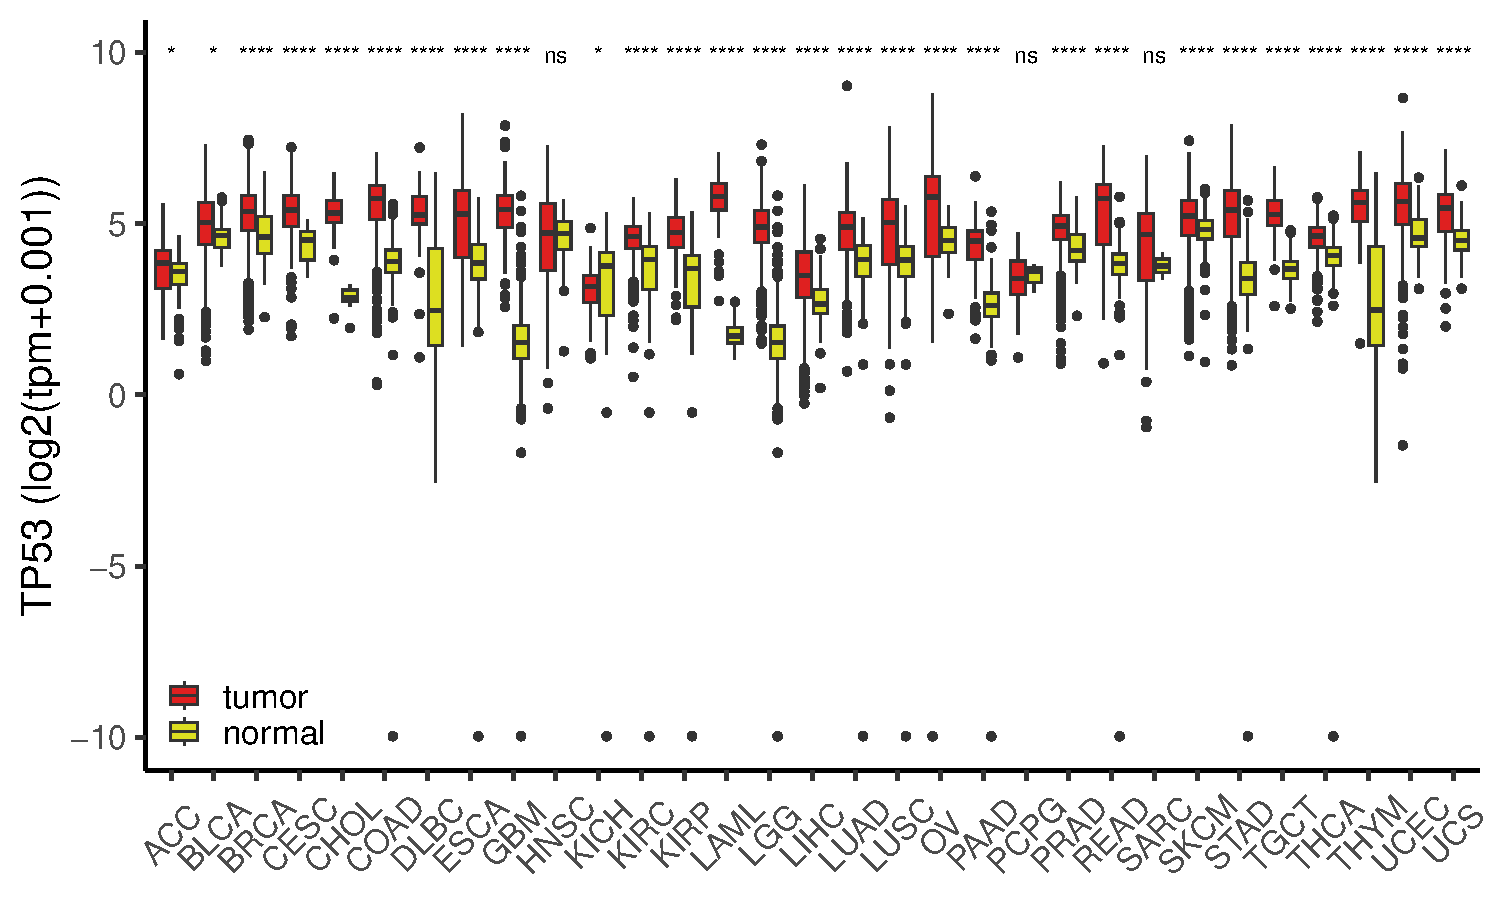
\includegraphics[width=0.8\linewidth]{_main_files/figure-latex/vis-toil-TvsN-1} 

}

\caption{The difference of mRNA TP53 across pan-cancer}\label{fig:vis-toil-TvsN}
\end{figure}

\subsubsection{\texorpdfstring{\href{https://openbiox.github.io/UCSCXenaShiny/reference/vis_toil_TvsN_cancer.html}{vis\_toil\_TvsN\_cancer()}}{vis\_toil\_TvsN\_cancer()}}\label{vis-toil-TvsN-cancer}

Compare molecular value between tumor and normal samples in one cancer. (\hyperref[m-vis_toil_TvsN]{Custom module})

\begin{itemize}
\tightlist
\item
  Basic use: \texttt{vis\_toil\_TvsN\_cancer(Gene=,\ data\_type=,\ Cancer=)}
\end{itemize}

\begin{Shaded}
\begin{Highlighting}[]
\FunctionTok{vis\_toil\_TvsN\_cancer}\NormalTok{(}\AttributeTok{Gene=}\StringTok{"TP53"}\NormalTok{, }\AttributeTok{data\_type =} \StringTok{"mRNA"}\NormalTok{, }\AttributeTok{Cancer =} \StringTok{"BRCA"}\NormalTok{)}
\end{Highlighting}
\end{Shaded}

\begin{figure}

{\centering 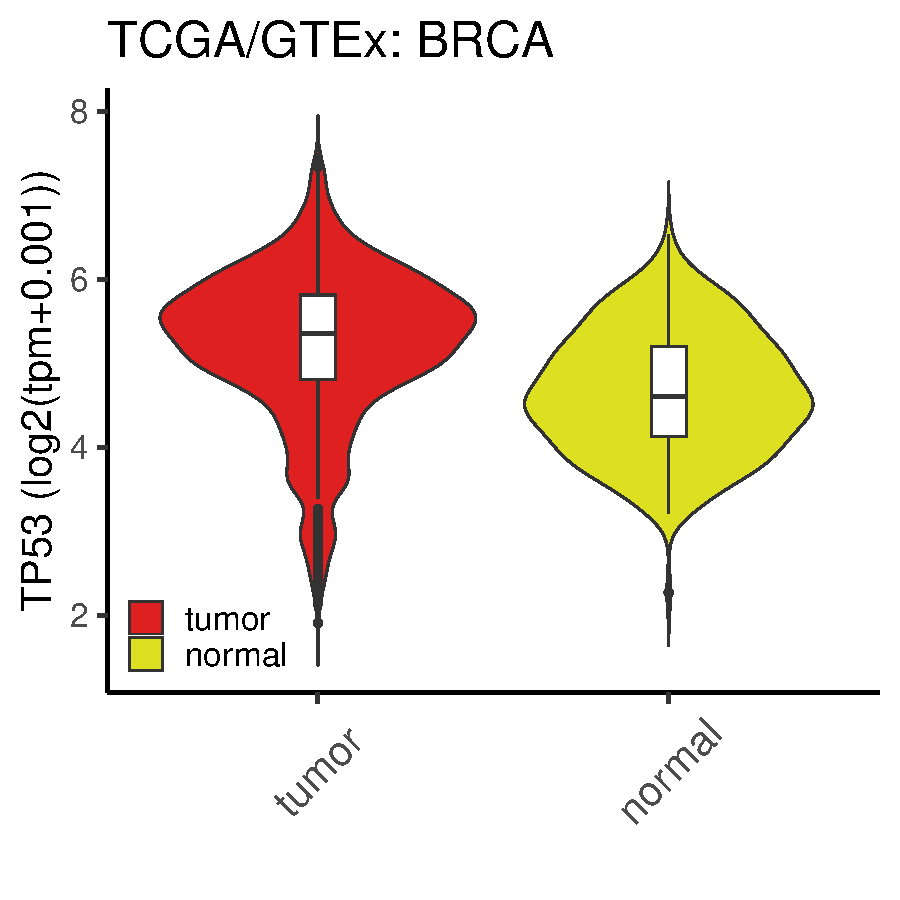
\includegraphics[width=0.8\linewidth]{_main_files/figure-latex/vis-toil-TvsN-cancer-1} 

}

\caption{The difference of mRNA TP53 in ACC cancer}\label{fig:vis-toil-TvsN-cancer}
\end{figure}

\subsubsection{\texorpdfstring{\href{https://openbiox.github.io/UCSCXenaShiny/refervis_pancan_anatomy.html}{vis\_pancan\_anatomy()}}{vis\_pancan\_anatomy()}}\label{vis-pancan-anatomy}

\begin{itemize}
\tightlist
\item
  Basic use: \texttt{vis\_pancan\_anatomy(Gene="TP53",\ Gender=,\ data\_type="mRNA")}
\end{itemize}

\begin{Shaded}
\begin{Highlighting}[]
\FunctionTok{library}\NormalTok{(gganatogram)}
\FunctionTok{vis\_pancan\_anatomy}\NormalTok{(}\AttributeTok{Gene =} \StringTok{"TP53"}\NormalTok{, }\AttributeTok{Gender =} \StringTok{"Male"}\NormalTok{, }\AttributeTok{data\_type=} \StringTok{"mRNA"}\NormalTok{)}
\end{Highlighting}
\end{Shaded}

\begin{verbatim}
## $plot
\end{verbatim}

\begin{figure}

{\centering 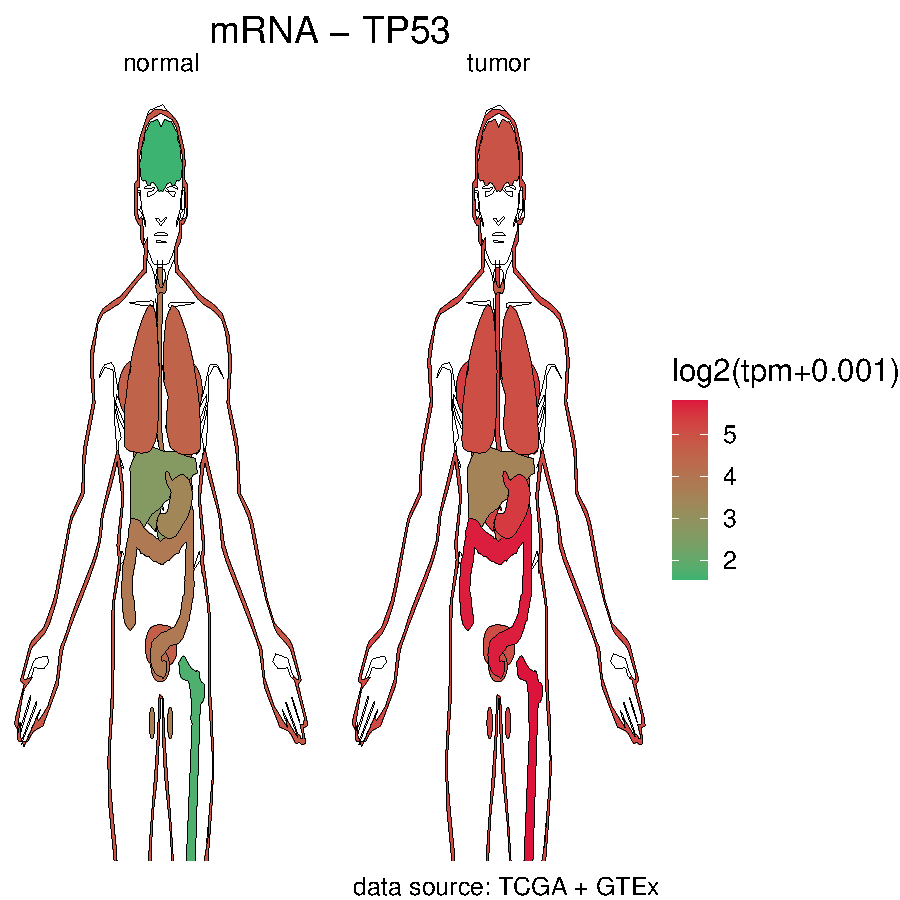
\includegraphics[width=0.8\linewidth]{_main_files/figure-latex/vis-pancan-anatomy-1} 

}

\caption{The difference of mRNA TP53 in Pan-cancer}\label{fig:vis-pancan-anatomy}
\end{figure}

\begin{verbatim}
## 
## $data
## # A tibble: 57 x 8
##    group       Median tissue type.x           type   organ           color value
##    <chr>        <dbl> <chr>  <fct>            <fct>  <chr>           <chr> <dbl>
##  1 ACC_normal    3.60 ACC    ACC_normal_GTEx  normal adrenal_gland   #41a~  3.60
##  2 ACC_tumor     3.85 ACC    ACC_tumor_TCGA   tumor  adrenal_gland   #41a~  3.85
##  3 BLCA_normal   4.65 BLCA   BLCA_normal_TCGA normal urinary_bladder oran~  4.65
##  4 BLCA_normal   4.65 BLCA   BLCA_normal_GTEx normal urinary_bladder oran~  4.65
##  5 BLCA_tumor    5.04 BLCA   BLCA_tumor_TCGA  tumor  urinary_bladder oran~  5.04
##  6 BRCA_normal   4.61 BRCA   BRCA_normal_GTEx normal breast          #41a~  4.61
##  7 BRCA_normal   4.61 BRCA   BRCA_normal_TCGA normal breast          #41a~  4.61
##  8 BRCA_tumor    5.36 BRCA   BRCA_tumor_TCGA  tumor  breast          #41a~  5.36
##  9 CHOL_normal   2.84 CHOL   CHOL_normal_TCGA normal gall_bladder    oran~  2.84
## 10 CHOL_tumor    5.31 CHOL   CHOL_tumor_TCGA  tumor  gall_bladder    oran~  5.31
## # i 47 more rows
\end{verbatim}

\subsubsection{\texorpdfstring{\href{https://openbiox.github.io/UCSCXenaShiny/reference/vis_toil_Mut.html}{vis\_toil\_Mut()}}{vis\_toil\_Mut()}}\label{vis-toil-Mut}

Compare molecular value between mutation and wild tumor samples across pan-cancer. (\hyperref[m-vis-toil-Mut]{Custom module})

\begin{itemize}
\tightlist
\item
  Basic use: \texttt{vis\_toil\_Mut(mut\_Gene=,\ Gene=,\ data\_type=)}
\end{itemize}

\begin{Shaded}
\begin{Highlighting}[]
\FunctionTok{vis\_toil\_Mut}\NormalTok{(}\AttributeTok{mut\_Gene =} \StringTok{"TP53"}\NormalTok{, }\AttributeTok{Gene =} \StringTok{"TNF"}\NormalTok{, }\AttributeTok{data\_type =} \StringTok{"mRNA"}\NormalTok{)}
\end{Highlighting}
\end{Shaded}

\begin{figure}

{\centering 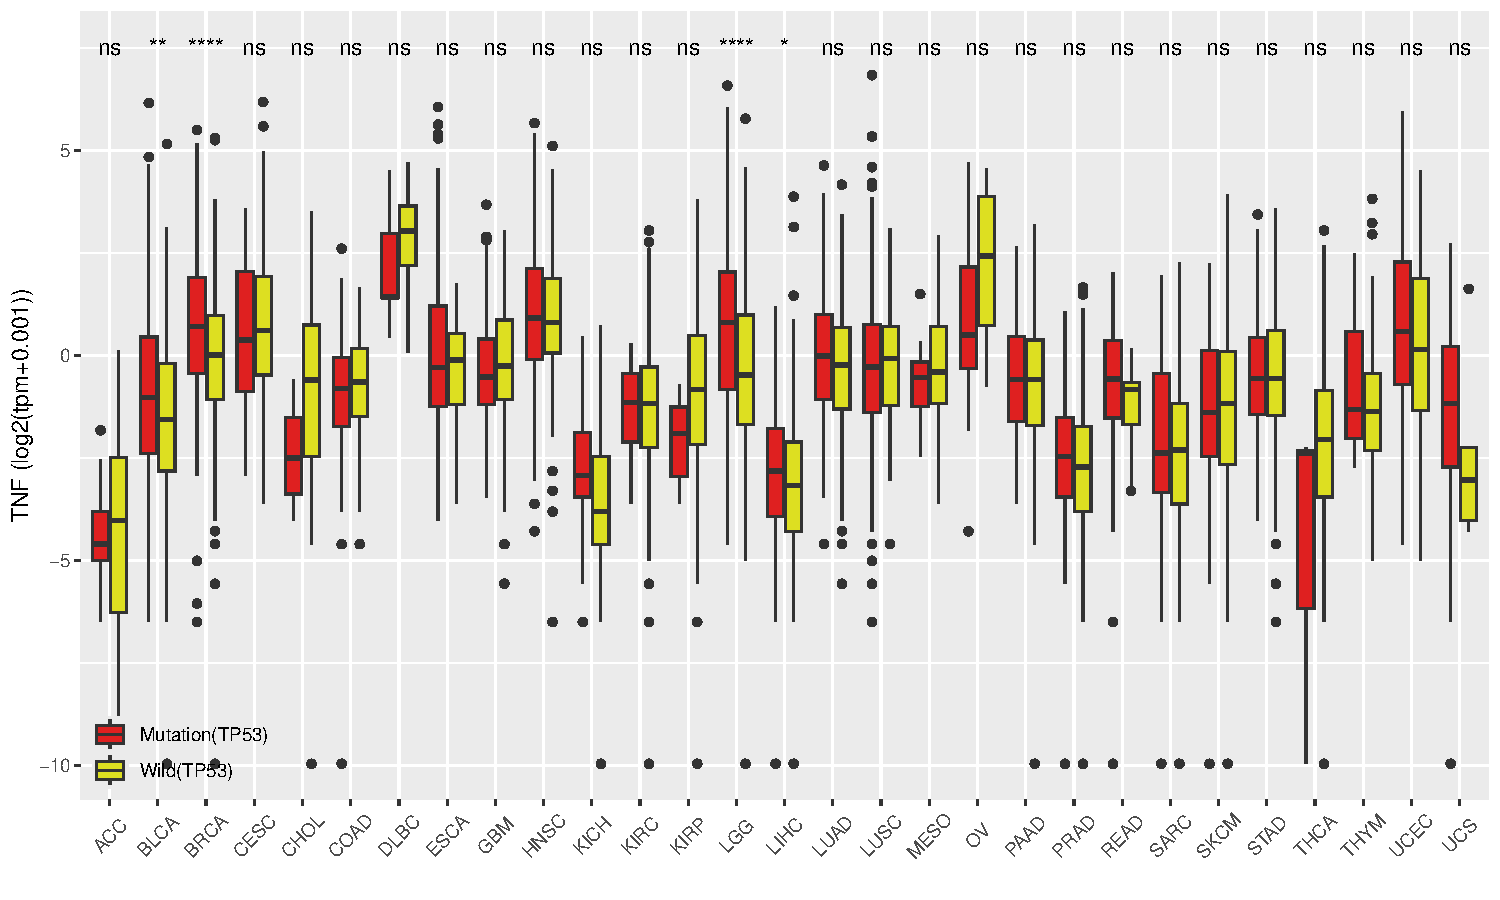
\includegraphics[width=0.8\linewidth]{_main_files/figure-latex/vis-toil-Mut-1} 

}

\caption{The difference of mRNA TNF between TP53-mut and TP53-wild tumor samples across pan-cancer}\label{fig:vis-toil-Mut}
\end{figure}

\subsubsection{\texorpdfstring{\href{https://openbiox.github.io/UCSCXenaShiny/reference/vis_toil_Mut_cancer.html}{vis\_toil\_Mut\_cancer()}}{vis\_toil\_Mut\_cancer()}}\label{vis-toil-Mut-cancer}

Compare molecular value between mutation and wild tumor samples in one cancer. (\hyperref[m-vis-toil-Mut]{Custom module})

\begin{itemize}
\tightlist
\item
  Basic use: \texttt{vis\_toil\_Mut\_cancer(Gene=,\ data\_type=,\ Cancer=)}
\end{itemize}

\begin{Shaded}
\begin{Highlighting}[]
\FunctionTok{vis\_toil\_Mut\_cancer}\NormalTok{(}\AttributeTok{mut\_Gene =} \StringTok{"TP53"}\NormalTok{, }\AttributeTok{Gene =} \StringTok{"TNF"}\NormalTok{, }\AttributeTok{data\_type =} \StringTok{"mRNA"}\NormalTok{, }\AttributeTok{Cancer =} \StringTok{"BRCA"}\NormalTok{)}
\end{Highlighting}
\end{Shaded}

\begin{figure}

{\centering 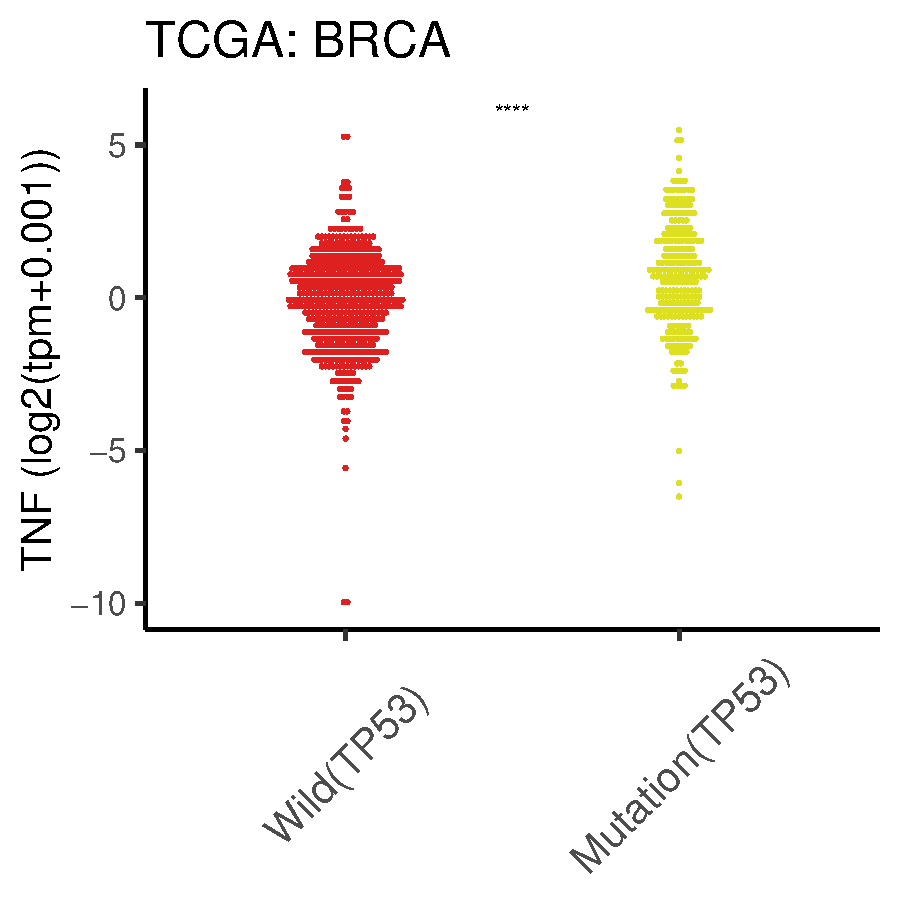
\includegraphics[width=0.8\linewidth]{_main_files/figure-latex/vis-toil-Mut-cancer-1} 

}

\caption{The difference of mRNA TNF between TP53-mut and TP53-wild tumor samples in BRCA cancer}\label{fig:vis-toil-Mut-cancer}
\end{figure}

\subsection{Correlation analysis}\label{correlation-analysis}

\subsubsection{\texorpdfstring{\href{https://openbiox.github.io/UCSCXenaShiny/reference/vis_gene_cor.html}{vis\_gene\_cor()}}{vis\_gene\_cor()}}\label{vis-gene-cor}

Calculate the correlation between two molecules value in tumor samples of pan-cancers. (\hyperref[m-vis-gene-cor]{Custom module})

\begin{itemize}
\tightlist
\item
  Basic use: \texttt{vis\_gene\_cor(Gene1=,\ data\_type1=,\ Gene2=,\ data\_type2=)}
\end{itemize}

\begin{Shaded}
\begin{Highlighting}[]
\FunctionTok{vis\_gene\_cor}\NormalTok{(}\AttributeTok{Gene1 =} \StringTok{"CSF1R"}\NormalTok{, }\AttributeTok{data\_type1 =} \StringTok{"mRNA"}\NormalTok{, }\AttributeTok{Gene2 =} \StringTok{"JAK3"}\NormalTok{, }\AttributeTok{data\_type2 =} \StringTok{"mRNA"}\NormalTok{)}
\end{Highlighting}
\end{Shaded}

\begin{figure}

{\centering 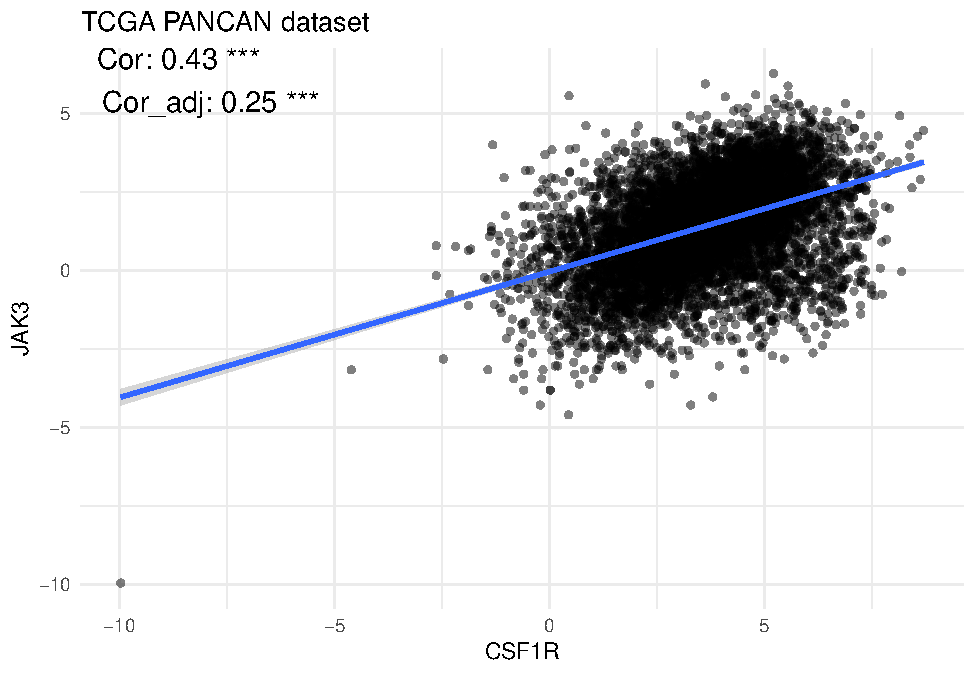
\includegraphics[width=0.8\linewidth]{_main_files/figure-latex/vis-gene-cor-1} 

}

\caption{The correlation between mRNA CSF1R and mRNA JAK3 in tumor samples of pan-cancers}\label{fig:vis-gene-cor}
\end{figure}

\subsubsection{\texorpdfstring{\href{https://openbiox.github.io/UCSCXenaShiny/reference/vis_gene_cor_cancer.html}{vis\_gene\_cor\_cancer()}}{vis\_gene\_cor\_cancer()}}\label{vis-gene-cor-cancer}

Calculate the correlation between two molecules value in tumor samples of one cancer. (\hyperref[m-vis-gene-cor]{Custom module})

\begin{itemize}
\tightlist
\item
  Basic use: \texttt{vis\_gene\_cor\_cancer(Gene1=,\ data\_type1=,\ Gene2=,\ data\_type2=,\ cancer\_choose=)}
\end{itemize}

\begin{Shaded}
\begin{Highlighting}[]
\FunctionTok{vis\_gene\_cor\_cancer}\NormalTok{(}\AttributeTok{Gene1 =} \StringTok{"CSF1R"}\NormalTok{, }\AttributeTok{data\_type1 =} \StringTok{"mRNA"}\NormalTok{, }
                    \AttributeTok{Gene2 =} \StringTok{"JAK3"}\NormalTok{, }\AttributeTok{data\_type2 =} \StringTok{"mRNA"}\NormalTok{, }
                    \AttributeTok{cancer\_choose =} \StringTok{"ACC"}\NormalTok{)}
\end{Highlighting}
\end{Shaded}

\begin{figure}

{\centering 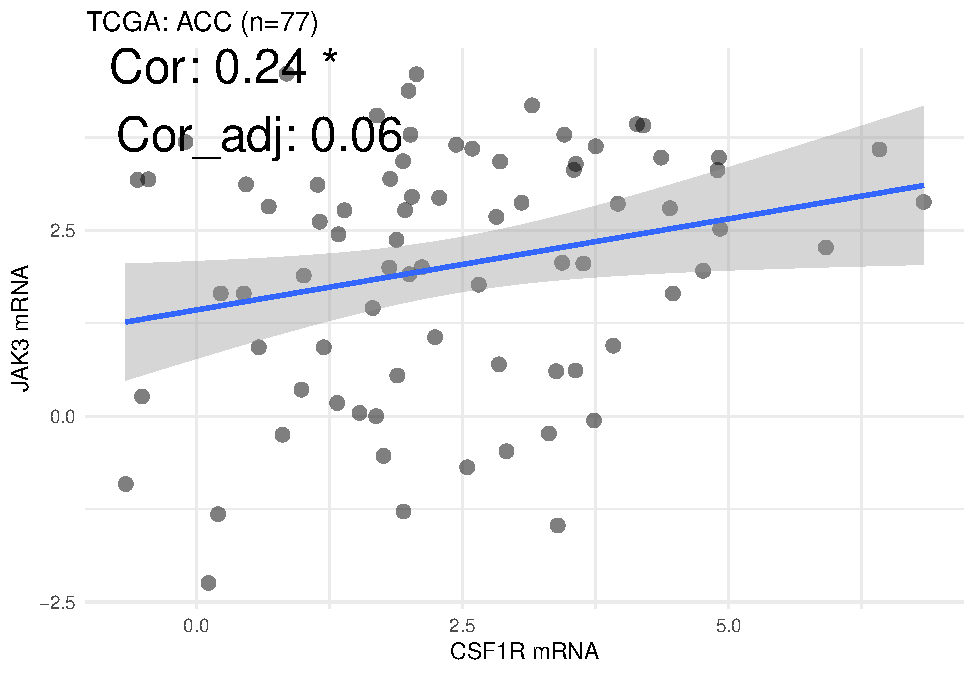
\includegraphics[width=0.8\linewidth]{_main_files/figure-latex/vis-gene-cor-cancer-1} 

}

\caption{The correlation between mRNA CSF1R and mRNA JAK3 in tumor samples of ACC cancer}\label{fig:vis-gene-cor-cancer}
\end{figure}

\subsubsection{\texorpdfstring{\href{https://openbiox.github.io/UCSCXenaShiny/reference/vis_gene_TIL_cor.html}{vis\_gene\_TIL\_cor()}}{vis\_gene\_TIL\_cor()}}\label{vis-gene-TIL-cor}

Calculate the correlation between one molecule and one type of TIL in tumor samples across pan-cancers. (\hyperref[m-vis-gene-TIL-cor]{Custom module})

\begin{itemize}
\tightlist
\item
  Basic use: \texttt{vis\_gene\_TIL\_cor(Gene=\ ,data\_type=\ ,sig=)}
\end{itemize}

\begin{Shaded}
\begin{Highlighting}[]
\NormalTok{tcga\_ids }\OtherTok{=} \FunctionTok{load\_data}\NormalTok{(}\StringTok{"pancan\_identifier\_help"}\NormalTok{)}
\FunctionTok{names}\NormalTok{(tcga\_ids}\SpecialCharTok{$}\NormalTok{id\_TIL)}
\end{Highlighting}
\end{Shaded}

\begin{verbatim}
## [1] "CIBERSORT"     "CIBERSORT-ABS" "EPIC"          "MCPCOUNTER"   
## [5] "QUANTISEQ"     "TIMER"         "XCELL"
\end{verbatim}

\begin{Shaded}
\begin{Highlighting}[]
\NormalTok{sig }\OtherTok{=} \FunctionTok{paste}\NormalTok{(tcga\_ids}\SpecialCharTok{$}\NormalTok{id\_TIL}\SpecialCharTok{$}\NormalTok{TIMER}\SpecialCharTok{$}\NormalTok{Level3,}
\NormalTok{            tcga\_ids}\SpecialCharTok{$}\NormalTok{id\_TIL}\SpecialCharTok{$}\NormalTok{TIMER}\SpecialCharTok{$}\NormalTok{Level2, }\AttributeTok{sep =} \StringTok{"\_"}\NormalTok{)}
\FunctionTok{vis\_gene\_TIL\_cor}\NormalTok{(}\AttributeTok{Gene =} \StringTok{"TP53"}\NormalTok{, }\AttributeTok{data\_type =} \StringTok{"mRNA"}\NormalTok{,}
                 \AttributeTok{sig =}\NormalTok{ sig)}
\end{Highlighting}
\end{Shaded}

\begin{figure}

{\centering 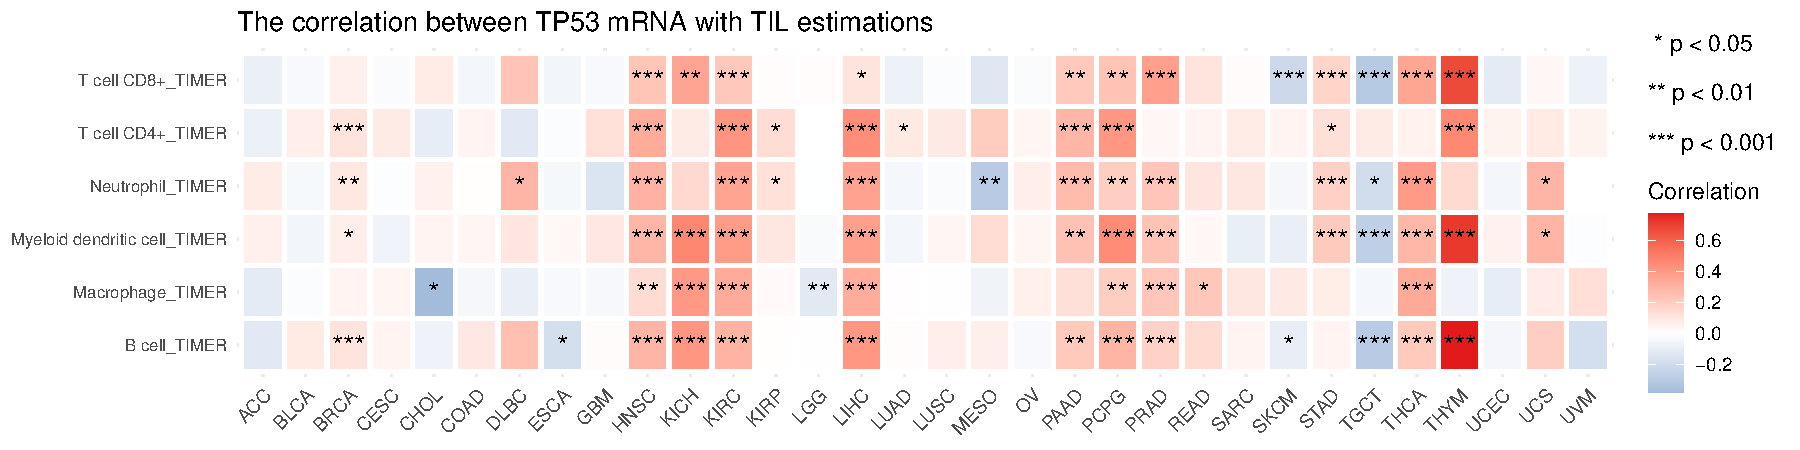
\includegraphics{_main_files/figure-latex/vis-gene-TIL-cor-1} 

}

\caption{The correlation between mRNA TP53 and TIMER TIL in tumor samples across pan-cancers}\label{fig:vis-gene-TIL-cor}
\end{figure}

\subsubsection{\texorpdfstring{\href{https://openbiox.github.io/UCSCXenaShiny/reference/vis_gene_immune_cor.html}{vis\_gene\_immune\_cor()}}{vis\_gene\_immune\_cor()}}\label{vis-gene-immune-cor}

Calculate the correlation between one molecule and one type of Immune signature in tumor samples across pan-cancers. (\hyperref[m-vis-gene-immune-cor]{Custom module})

\begin{itemize}
\tightlist
\item
  Basic use: \texttt{vis\_gene\_immune\_cor(Gene=\ ,data\_type=\ ,sig=)}
\end{itemize}

\begin{Shaded}
\begin{Highlighting}[]
\NormalTok{tcga\_pan\_immune\_signature }\OtherTok{\textless{}{-}} \FunctionTok{load\_data}\NormalTok{(}\StringTok{"tcga\_pan\_immune\_signature"}\NormalTok{)}
\FunctionTok{table}\NormalTok{(tcga\_pan\_immune\_signature}\SpecialCharTok{$}\NormalTok{Source)}
\end{Highlighting}
\end{Shaded}

\begin{verbatim}
## 
## Attractors     Bindea    c7atoms  Cibersort        ICR       Wolf      Yasin 
##          9         25         32         20          3         68          3
\end{verbatim}

\begin{Shaded}
\begin{Highlighting}[]
\FunctionTok{vis\_gene\_immune\_cor}\NormalTok{(}\AttributeTok{Gene =} \StringTok{"TP53"}\NormalTok{, }\AttributeTok{data\_type =} \StringTok{"mRNA"}\NormalTok{,}
                    \AttributeTok{Immune\_sig\_type =} \StringTok{"Cibersort"}\NormalTok{)}
\end{Highlighting}
\end{Shaded}

\begin{figure}

{\centering 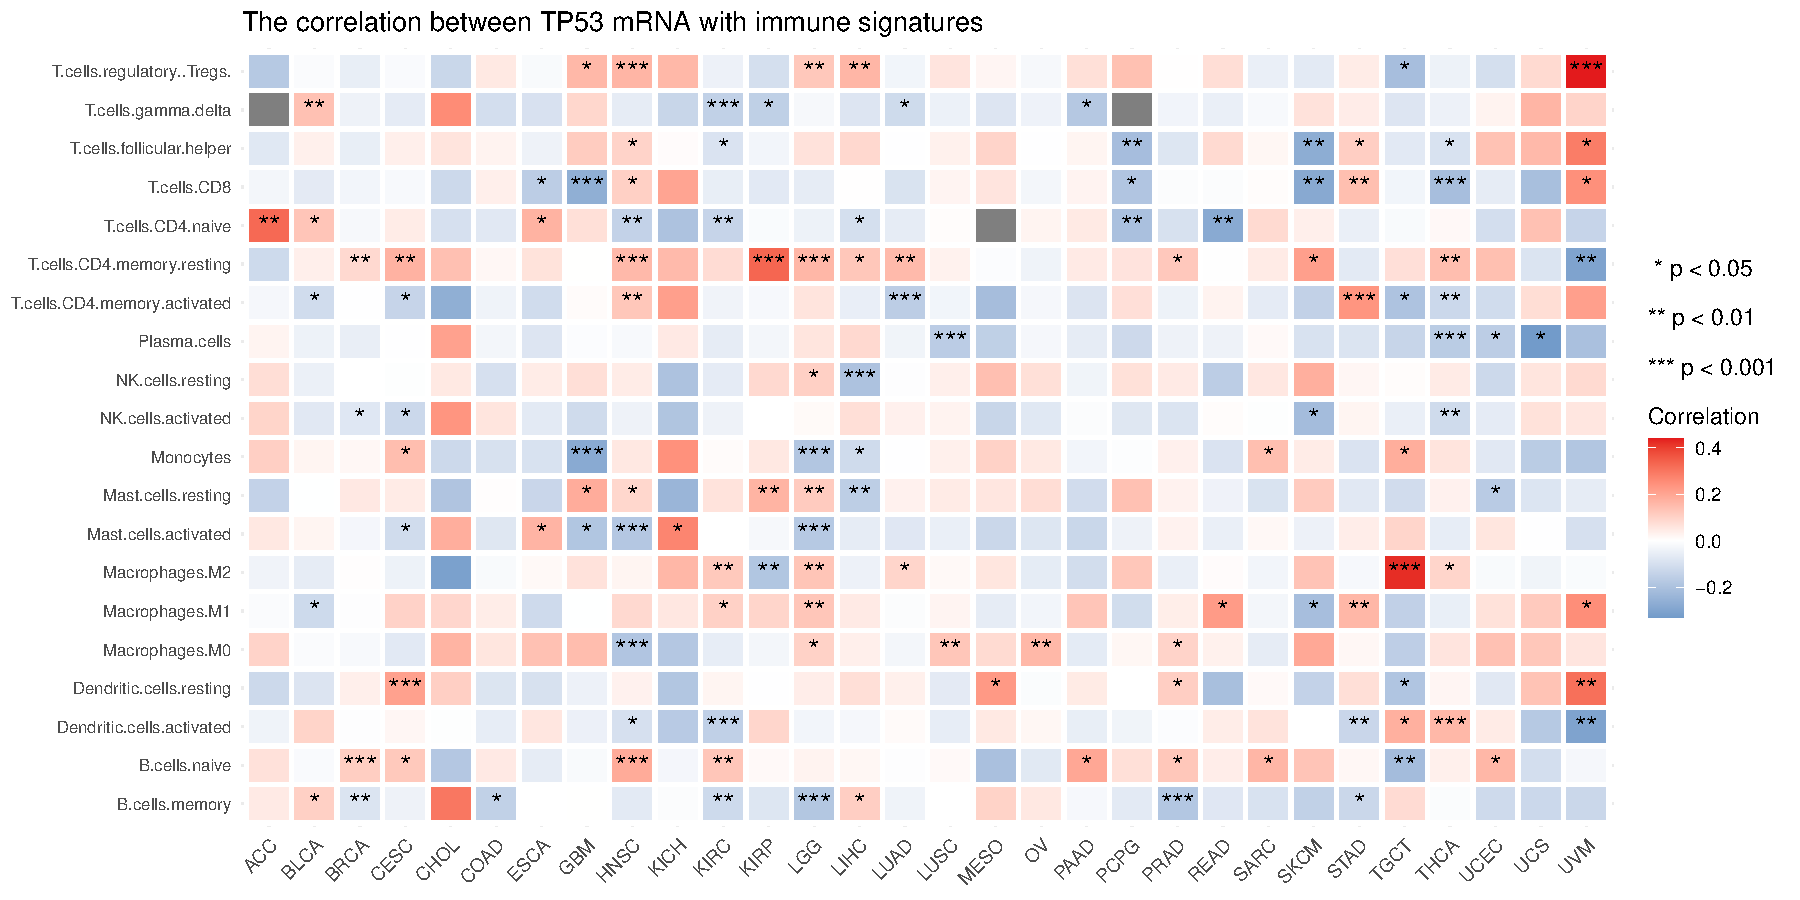
\includegraphics{_main_files/figure-latex/vis-gene-immune-cor-1} 

}

\caption{The correlation between mRNA TP53 and Cibersort signature in tumor samples across pan-cancers}\label{fig:vis-gene-immune-cor}
\end{figure}

\subsubsection{\texorpdfstring{\href{https://openbiox.github.io/UCSCXenaShiny/reference/vis_gene_tmb_cor.html}{vis\_gene\_tmb\_cor()}}{vis\_gene\_tmb\_cor()}}\label{vis-gene-tmb-cor}

Calculate the correlation between one molecule and TMB score in tumor samples across pan-cancers. (\hyperref[m-vis-gene-index]{Custom module})

\begin{itemize}
\tightlist
\item
  Basic use: \texttt{vis\_gene\_tmb\_cor(Gene=\ ,\ data\_type=\ )}
\end{itemize}

\begin{Shaded}
\begin{Highlighting}[]
\FunctionTok{vis\_gene\_tmb\_cor}\NormalTok{(}\AttributeTok{Gene =} \StringTok{"TP53"}\NormalTok{, }\AttributeTok{data\_type =} \StringTok{"mRNA"}\NormalTok{)}
\end{Highlighting}
\end{Shaded}

\begin{figure}

{\centering 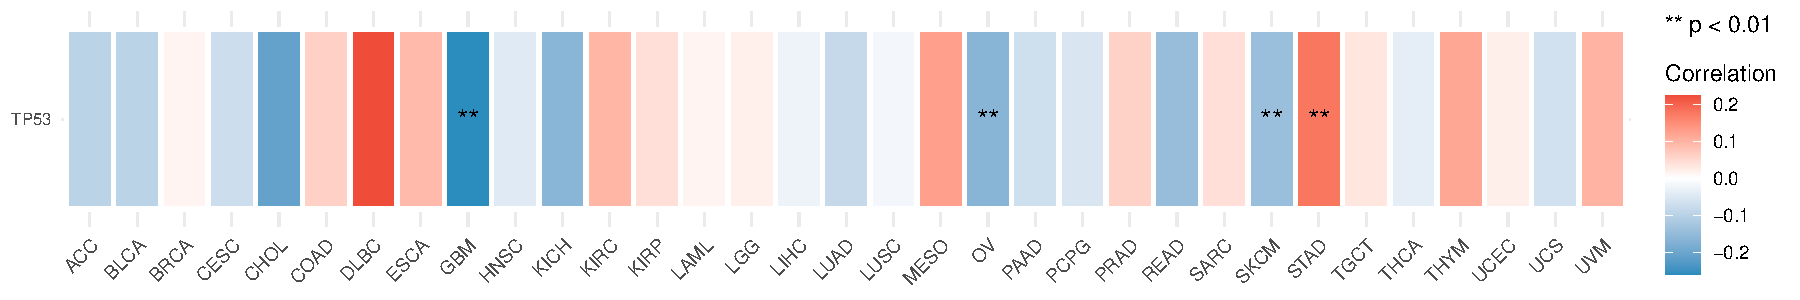
\includegraphics{_main_files/figure-latex/vis-gene-tmb-cor-1} 

}

\caption{The correlation between mRNA TP53 and TMB score in tumor samples across pan-cancers}\label{fig:vis-gene-tmb-cor}
\end{figure}

\subsubsection{\texorpdfstring{\href{https://openbiox.github.io/UCSCXenaShiny/reference/vis_gene_msi_cor.html}{vis\_gene\_msi\_cor()}}{vis\_gene\_msi\_cor()}}\label{vis-gene-msi-cor}

Calculate the correlation between one molecule and MSI score in tumor samples across pan-cancers. (\hyperref[m-vis-gene-index]{Custom module})

\begin{itemize}
\tightlist
\item
  Basic use: \texttt{vis\_gene\_msi\_cor(Gene=\ ,\ data\_type=\ )}
\end{itemize}

\begin{Shaded}
\begin{Highlighting}[]
\FunctionTok{vis\_gene\_msi\_cor}\NormalTok{(}\AttributeTok{Gene =} \StringTok{"TP53"}\NormalTok{, }\AttributeTok{data\_type =} \StringTok{"mRNA"}\NormalTok{)}
\end{Highlighting}
\end{Shaded}

\begin{figure}

{\centering 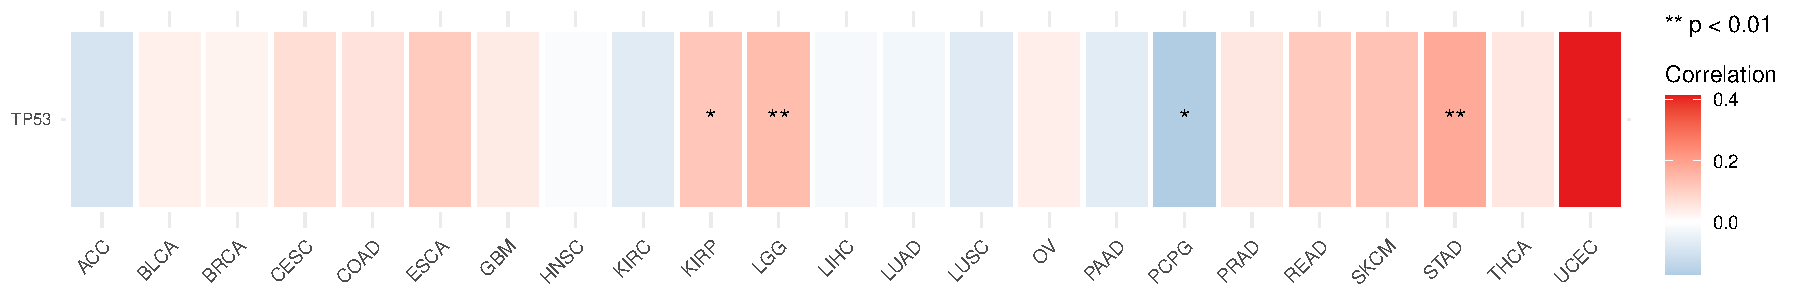
\includegraphics{_main_files/figure-latex/vis-gene-msi-cor-1} 

}

\caption{The correlation between mRNA TP53 and MSI score in tumor samples across pan-cancers}\label{fig:vis-gene-msi-cor}
\end{figure}

\subsubsection{\texorpdfstring{\href{https://openbiox.github.io/UCSCXenaShiny/reference/vis_gene_stemness_cor.html}{vis\_gene\_stemness\_cor()}}{vis\_gene\_stemness\_cor()}}\label{vis-gene-stemness-cor}

Calculate the correlation between one molecule and stemness score in tumor samples across pan-cancers. (\hyperref[m-vis-gene-index]{Custom module})

\begin{itemize}
\tightlist
\item
  Basic use: \texttt{vis\_gene\_stemness\_cor(Gene=\ ,\ data\_type=\ )}
\end{itemize}

\begin{Shaded}
\begin{Highlighting}[]
\FunctionTok{vis\_gene\_stemness\_cor}\NormalTok{(}\AttributeTok{Gene =} \StringTok{"TP53"}\NormalTok{, }\AttributeTok{data\_type =} \StringTok{"mRNA"}\NormalTok{)}
\end{Highlighting}
\end{Shaded}

\begin{figure}

{\centering 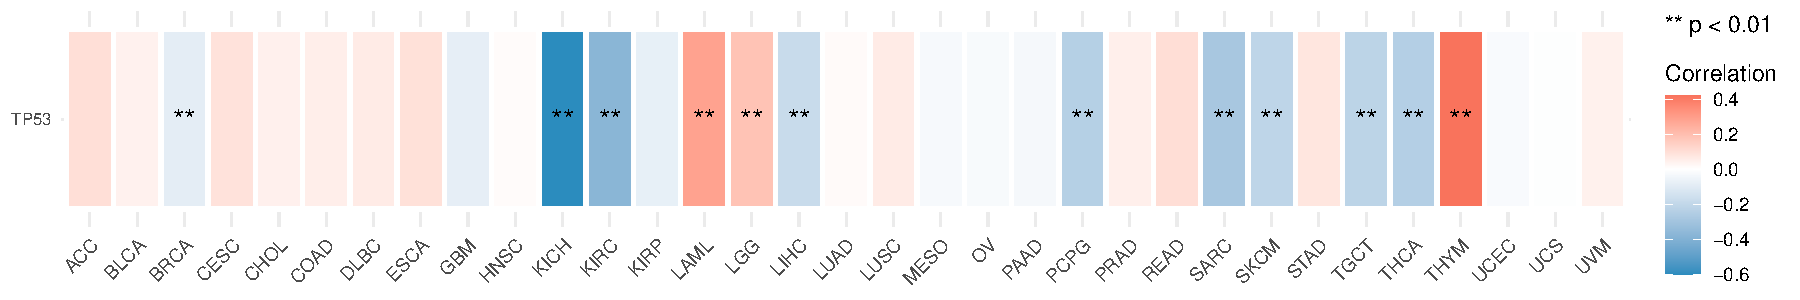
\includegraphics{_main_files/figure-latex/vis-gene-stemness-cor-1} 

}

\caption{The correlation between mRNA TP53 and stemness score in tumor samples across pan-cancers}\label{fig:vis-gene-stemness-cor}
\end{figure}

\subsubsection{\texorpdfstring{\href{https://openbiox.github.io/UCSCXenaShiny/reference/vis_gene_pw_cor.html}{vis\_gene\_pw\_cor()}}{vis\_gene\_pw\_cor()}}\label{vis-gene-pw-cor}

Calculate the correlation between one molecule and pathway score in tumor samples of one cancer. (\hyperref[m-vis-gene-pw-cor]{Custom module})

\begin{itemize}
\tightlist
\item
  Basic use: \texttt{vis\_gene\_pw\_cor(Gene=\ ,\ data\_type=\ )}
\end{itemize}

\begin{Shaded}
\begin{Highlighting}[]
\FunctionTok{vis\_gene\_pw\_cor}\NormalTok{(}\AttributeTok{Gene =} \StringTok{"TP53"}\NormalTok{, }\AttributeTok{data\_type =} \StringTok{"mRNA"}\NormalTok{, }
                \AttributeTok{pw\_name =} \StringTok{"HALLMARK\_ADIPOGENESIS"}\NormalTok{,}
                \AttributeTok{cancer\_choose =} \StringTok{"ACC"}\NormalTok{)}
\end{Highlighting}
\end{Shaded}

\begin{figure}

{\centering 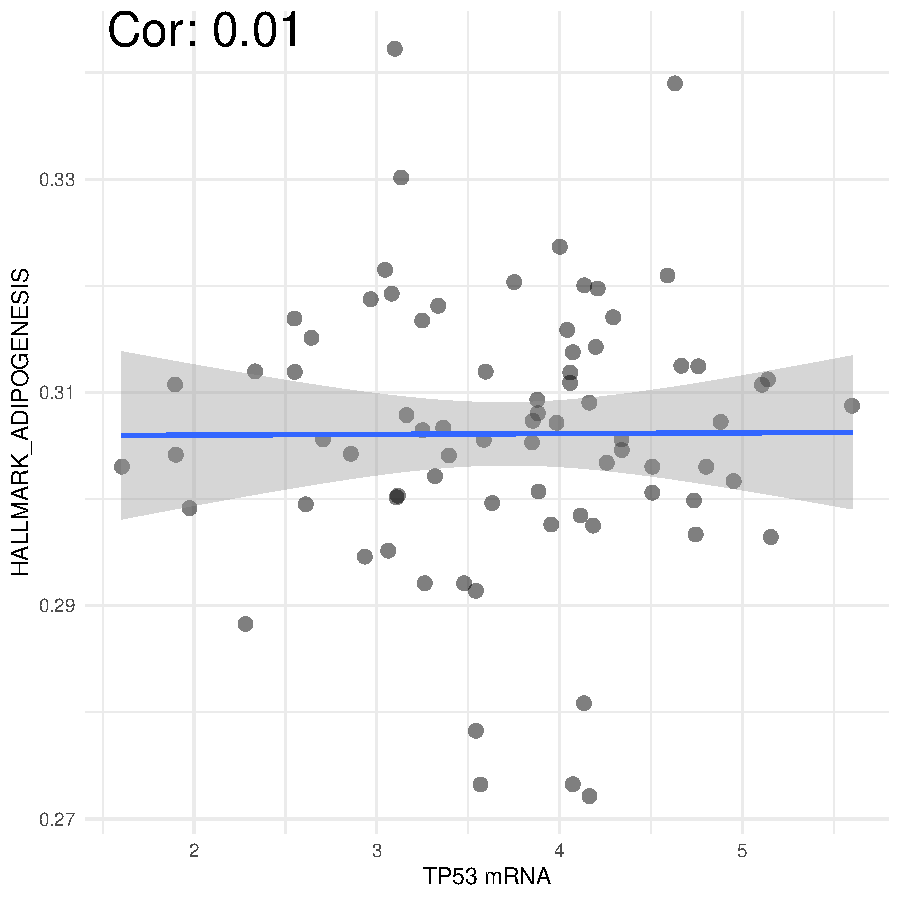
\includegraphics{_main_files/figure-latex/vis-gene-pw-cor-1} 

}

\caption{The correlation between mRNA TP53 and pathway score in tumor samples in ACC cancer}\label{fig:vis-gene-pw-cor}
\end{figure}

\subsection{Survival analysis}\label{survival-analysis}

\subsubsection{\texorpdfstring{\href{https://openbiox.github.io/UCSCXenaShiny/reference/tcga_surv_plot.html}{tcga\_surv\_plot()}}{tcga\_surv\_plot()}}\label{tcga-surv-plot}

Perform the log-rank test of one molecule for one cancer. (\hyperref[m-tcga-surv-plot]{Custom module})

\begin{itemize}
\tightlist
\item
  Basic use: \texttt{tcga\_surv\_plot(data=,\ time=\ ,\ status=\ )}
\end{itemize}

\begin{Shaded}
\begin{Highlighting}[]
\CommentTok{\# Firstly, prepare the molecular value as well as survival data}
\NormalTok{data }\OtherTok{\textless{}{-}} \FunctionTok{tcga\_surv\_get}\NormalTok{(}\AttributeTok{item =} \StringTok{"TP53"}\NormalTok{,}\AttributeTok{profile =} \StringTok{"mRNA"}\NormalTok{,}
                      \AttributeTok{TCGA\_cohort =} \StringTok{"LUAD"}\NormalTok{)}
\FunctionTok{head}\NormalTok{(data)}
\end{Highlighting}
\end{Shaded}

\begin{verbatim}
## # A tibble: 6 x 13
##   sampleID      value    OS OS.time   DSS DSS.time   DFI DFI.time   PFI PFI.time
##   <chr>         <dbl> <dbl>   <dbl> <dbl>    <dbl> <dbl>    <dbl> <dbl>    <dbl>
## 1 TCGA-05-4420~  4.51     0     912     0      912     0      912     0      912
## 2 TCGA-91-6840~  5.90     0     372     0      372     0      372     0      372
## 3 TCGA-44-6778~  5.30     0    1864     0     1864     0     1864     0     1864
## 4 TCGA-67-3774~  5.22     0     385     0      385    NA       NA     0      385
## 5 TCGA-64-1679~  5.46     0    2488     0     2488     0     2488     0     2488
## 6 TCGA-55-6982~  4.54     1     995     1      995    NA       NA     1      183
## # i 3 more variables: gender <chr>, age <dbl>, stage <chr>
\end{verbatim}

\begin{Shaded}
\begin{Highlighting}[]
\FunctionTok{tcga\_surv\_plot}\NormalTok{(data, }\AttributeTok{time =} \StringTok{"DSS.time"}\NormalTok{, }\AttributeTok{status =} \StringTok{"DSS"}\NormalTok{) }\CommentTok{\# OS/DSS/DFI/PFI}
\end{Highlighting}
\end{Shaded}

\begin{figure}

{\centering 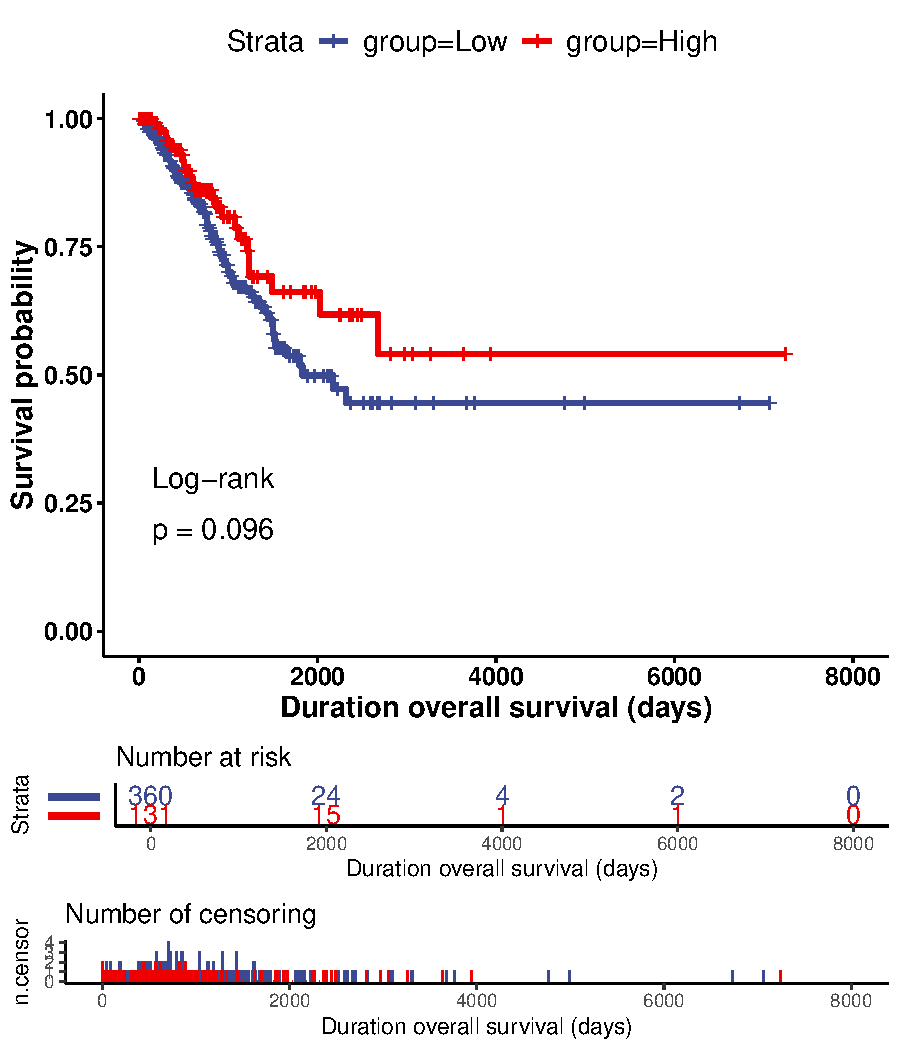
\includegraphics{_main_files/figure-latex/tcga-surv-plot-1} 

}

\caption{The log-rank test (DSS) of mRNA TP53 for LUAD cancer}\label{fig:tcga-surv-plot}
\end{figure}

\begin{quote}
By default, the median data of molecular data is used to divided into two groups for log-rank test. It can be modified in corresponding paramters.
\end{quote}

\subsubsection{\texorpdfstring{\href{https://openbiox.github.io/UCSCXenaShiny/reference/vis_unicox_tree.html}{vis\_unicox\_tree()}}{vis\_unicox\_tree()}}\label{vis-unicox-tree}

Perform the Cox regression analysis of one molecule across pan-cancers. (\hyperref[m-vis-unicox-tree]{Custom module})

\begin{itemize}
\tightlist
\item
  Basic use: \texttt{vis\_unicox\_tree(Gene=\ ,\ data\_type=\ ,\ measure=)}
\end{itemize}

\begin{Shaded}
\begin{Highlighting}[]
\FunctionTok{vis\_unicox\_tree}\NormalTok{(}\AttributeTok{Gene =} \StringTok{"PTEN"}\NormalTok{, }\AttributeTok{data\_type =} \StringTok{"mRNA"}\NormalTok{, }\AttributeTok{measure =} \StringTok{"OS"}\NormalTok{)}
\end{Highlighting}
\end{Shaded}

\begin{figure}

{\centering 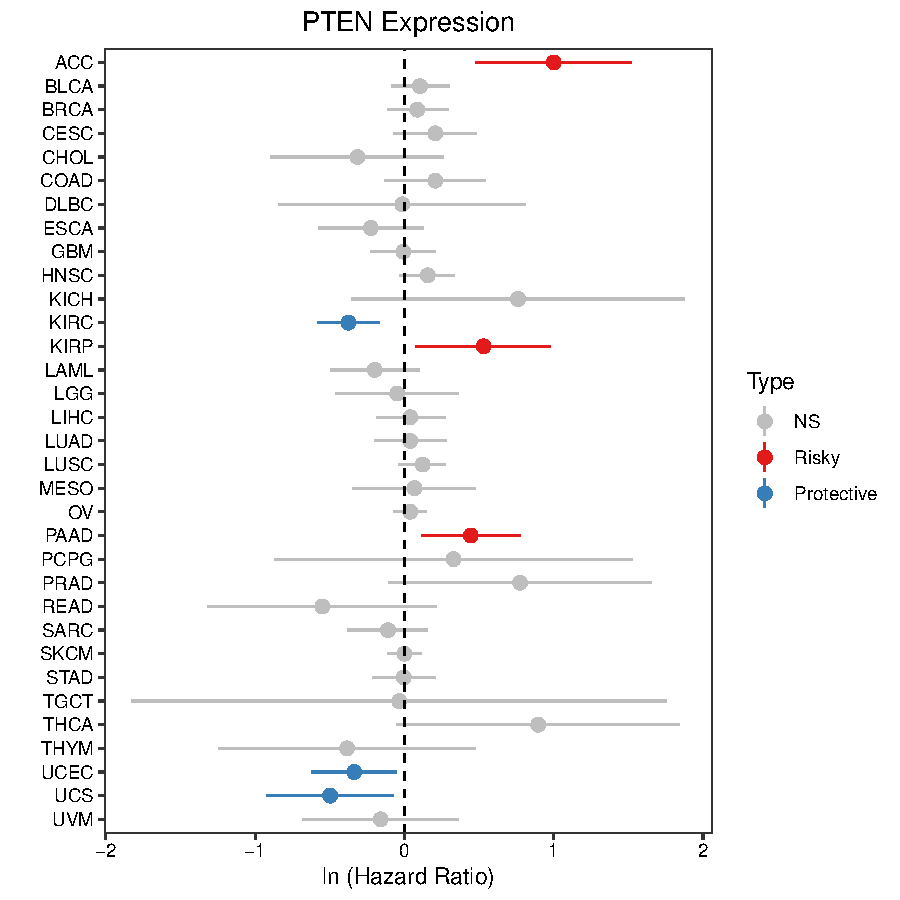
\includegraphics{_main_files/figure-latex/vis-unicox-tree-1} 

}

\caption{The Cox regression analysis (OS) of mRNA PTEN across pan-cancers}\label{fig:vis-unicox-tree}
\end{figure}

\begin{quote}
By default, the median data of molecular data is used to divided into two groups for Cox regression analysis. It can be modified in corresponding paramters.
\end{quote}

\subsection{Dimension reduction}\label{dimension-reduction}

\subsubsection{\texorpdfstring{\href{https://openbiox.github.io/UCSCXenaShiny/reference/vis_dim_dist.html}{vis\_dim\_dist()}}{vis\_dim\_dist()}}\label{vis-dim-dist}

Perform dimension reduction analysis of multiple molecules for samples in groups. (\hyperref[m-vis-dim-dist]{Custom module})

\begin{itemize}
\tightlist
\item
  Basic use: \texttt{vis\_dim\_dist(ids=,\ data\_type=\ ,group\_info=\ )}
\end{itemize}

\begin{Shaded}
\begin{Highlighting}[]
\CommentTok{\# Firstly, prepare the grouping information of samples }
\NormalTok{group\_info }\OtherTok{=}\NormalTok{ tcga\_clinical\_fine }\SpecialCharTok{\%\textgreater{}\%} 
\NormalTok{  dplyr}\SpecialCharTok{::}\FunctionTok{filter}\NormalTok{(Cancer}\SpecialCharTok{==}\StringTok{"BRCA"}\NormalTok{) }\SpecialCharTok{\%\textgreater{}\%} 
\NormalTok{  dplyr}\SpecialCharTok{::}\FunctionTok{select}\NormalTok{(Sample, Code) }\SpecialCharTok{\%\textgreater{}\%} 
\NormalTok{  dplyr}\SpecialCharTok{::}\FunctionTok{rename}\NormalTok{(}\AttributeTok{Group=}\NormalTok{Code)}
\FunctionTok{head}\NormalTok{(group\_info)}
\end{Highlighting}
\end{Shaded}

\begin{verbatim}
## # A tibble: 6 x 2
##   Sample          Group
##   <chr>           <chr>
## 1 TCGA-3C-AAAU-01 TP   
## 2 TCGA-3C-AALI-01 TP   
## 3 TCGA-3C-AALJ-01 TP   
## 4 TCGA-3C-AALK-01 TP   
## 5 TCGA-4H-AAAK-01 TP   
## 6 TCGA-5L-AAT0-01 TP
\end{verbatim}

\begin{Shaded}
\begin{Highlighting}[]
\NormalTok{ids }\OtherTok{=} \FunctionTok{c}\NormalTok{(}\StringTok{"TP53"}\NormalTok{, }\StringTok{"KRAS"}\NormalTok{, }\StringTok{"PTEN"}\NormalTok{, }\StringTok{"MDM2"}\NormalTok{, }\StringTok{"CDKN1A"}\NormalTok{)}
\FunctionTok{vis\_dim\_dist}\NormalTok{(}\AttributeTok{ids =}\NormalTok{ ids, }\AttributeTok{data\_type =} \StringTok{"mRNA"}\NormalTok{, }
             \AttributeTok{group\_info=}\NormalTok{ group\_info)}
\end{Highlighting}
\end{Shaded}

\begin{figure}

{\centering 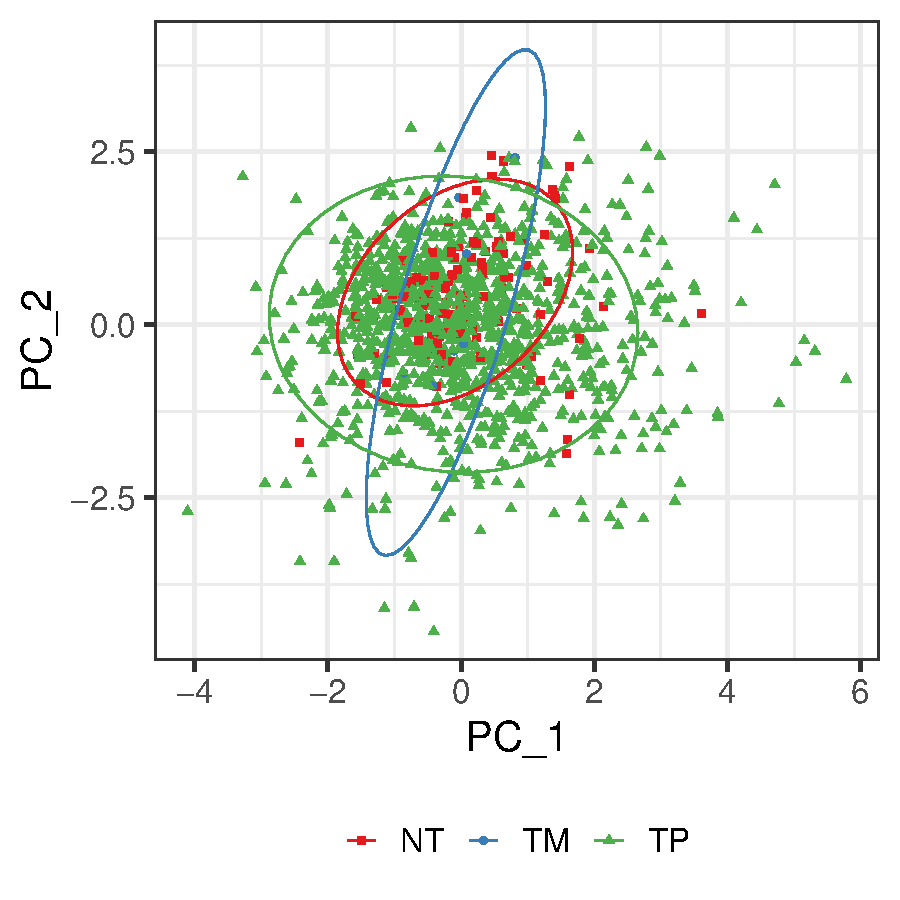
\includegraphics{_main_files/figure-latex/vis-dim-dist-1} 

}

\caption{The dimension reduction analysis (PCA) of 5 mRNA molcules in BRCA cancer samples grouped by tissue codes}\label{fig:vis-dim-dist}
\end{figure}

\section{PCAWG analysis}\label{pcawg-analysis}

\begin{table}

\caption{\label{tab:analyze-pcawg-func}Specilized functions to analyze PCAWG molecular data}
\centering
\begin{tabular}[t]{lll}
\toprule
Database & Type & Function\\
\midrule
PCAWG & Comparison & vis\_pcawg\_dist()\\
PCAWG & Correlation & vis\_pcawg\_gene\_cor()\\
PCAWG & Survival & vis\_pcawg\_unicox\_tree()\\
\bottomrule
\end{tabular}
\end{table}

\subsection{Comparsion analysis}\label{comparsion-analysis}

\subsubsection{\texorpdfstring{\href{https://openbiox.github.io/UCSCXenaShiny/reference/vis_pcawg_dist.html}{vis\_pcawg\_dist()}}{vis\_pcawg\_dist()}}\label{vis-pcawg-dist}

Compare molecular value between tumor and normal samples across pan-cancer. (\hyperref[m-vis-pcawg-dist]{Custom module})

\begin{itemize}
\tightlist
\item
  Basic use: \texttt{vis\_pcawg\_dist(Gene=\ ,data\_type=\ )}
\end{itemize}

\begin{Shaded}
\begin{Highlighting}[]
\FunctionTok{vis\_pcawg\_dist}\NormalTok{(}\AttributeTok{Gene =} \StringTok{"TP53"}\NormalTok{, }\AttributeTok{data\_type =} \StringTok{"mRNA"}\NormalTok{)}
\end{Highlighting}
\end{Shaded}

\begin{center}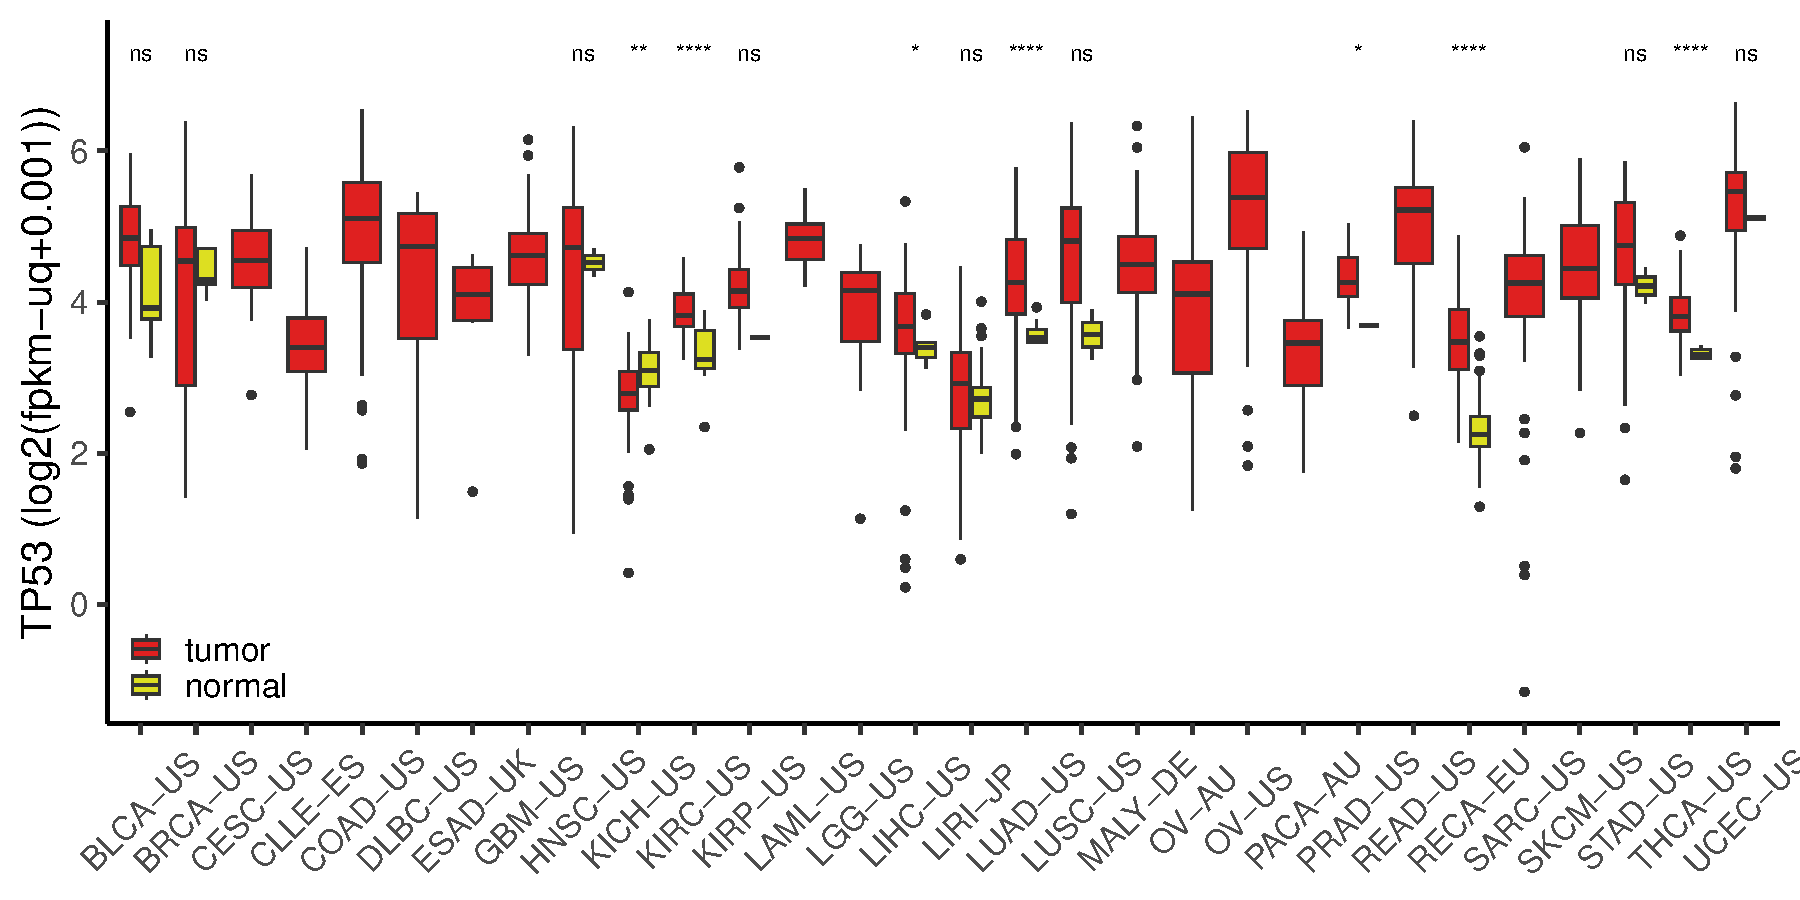
\includegraphics{_main_files/figure-latex/vis-pcawg-dist-1} \end{center}

\subsection{Correlation analysis}\label{correlation-analysis-1}

\subsubsection{\texorpdfstring{\href{https://openbiox.github.io/UCSCXenaShiny/reference/vis_pcawg_gene_cor.html}{vis\_pcawg\_gene\_cor()}}{vis\_pcawg\_gene\_cor()}}\label{vis-pcawg-gene-cor}

Calculate the correlation between two molecules value in tumor samples of one cancer. (\hyperref[m-vis-pcawg-gene-cor]{Custom module})

\begin{itemize}
\tightlist
\item
  Basic use: \texttt{vis\_pcawg\_gene\_cor(Gene1=\ ,data\_type1\ =\ ,Gene2\ =\ ,data\_type2\ =\ ,dcc\_project\_code\_choose=)}
\end{itemize}

\begin{Shaded}
\begin{Highlighting}[]
\FunctionTok{vis\_pcawg\_gene\_cor}\NormalTok{(}\AttributeTok{Gene1 =} \StringTok{"CSF1R"}\NormalTok{, }\AttributeTok{data\_type1 =} \StringTok{"mRNA"}\NormalTok{,}
                   \AttributeTok{Gene2 =} \StringTok{"JAK3"}\NormalTok{, }\AttributeTok{data\_type2 =} \StringTok{"mRNA"}\NormalTok{,}
                   \AttributeTok{dcc\_project\_code\_choose =} \StringTok{"BLCA{-}US"}\NormalTok{)}
\end{Highlighting}
\end{Shaded}

\begin{center}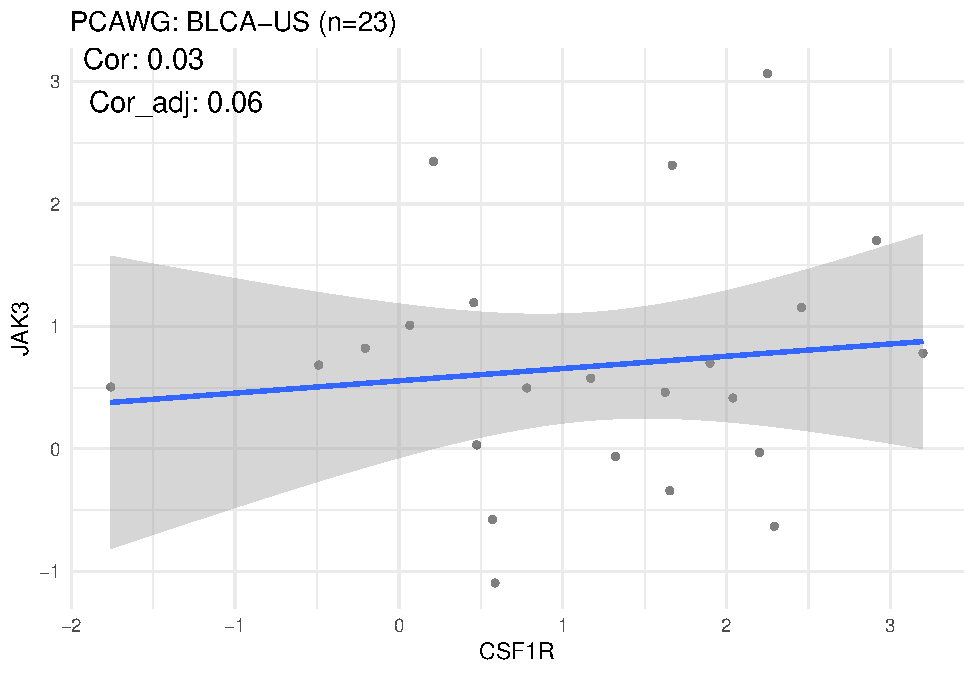
\includegraphics[width=0.8\linewidth]{_main_files/figure-latex/vis-pcawg-gene_cor-1} \end{center}

\subsection{Survival analysis}\label{survival-analysis-1}

\subsubsection{\texorpdfstring{\href{https://openbiox.github.io/UCSCXenaShiny/reference/vis_pcawg_unicox_tree.html}{vis\_pcawg\_unicox\_tree()}}{vis\_pcawg\_unicox\_tree()}}\label{vis-pcawg-unicox-tree}

Perform the Cox regression analysis (OS) of one molecule across pan-cancers. (\hyperref[m-vis-pcawg-unicox-tree]{Custom module})

\begin{itemize}
\tightlist
\item
  Basic use: \texttt{vis\_pcawg\_unicox\_tree(Gene=\ ,\ data\_type=\ )}
\end{itemize}

\begin{Shaded}
\begin{Highlighting}[]
\FunctionTok{vis\_pcawg\_unicox\_tree}\NormalTok{(}\AttributeTok{Gene =} \StringTok{"TP53"}\NormalTok{, }\AttributeTok{data\_type =} \StringTok{"mRNA"}\NormalTok{)}
\end{Highlighting}
\end{Shaded}

\begin{figure}

{\centering 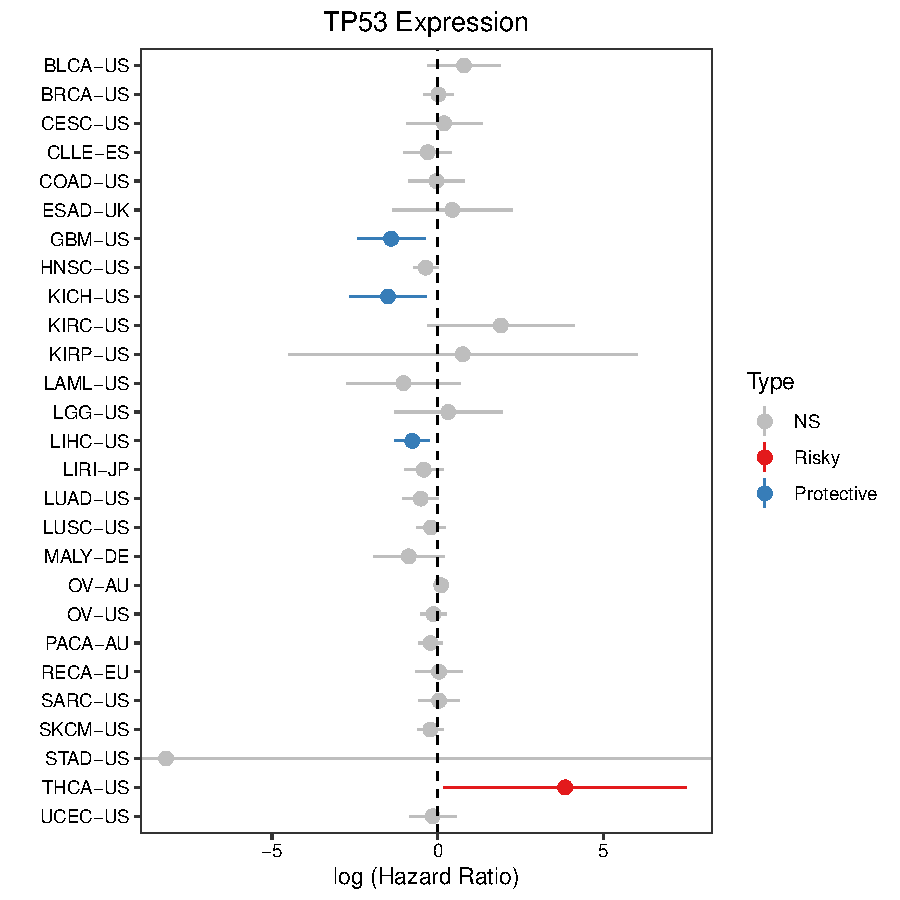
\includegraphics{_main_files/figure-latex/vis-pcawg-unicox-tree-1} 

}

\caption{The Cox regression analysis (OS) of mRNA TP53 across pan-cancers}\label{fig:vis-pcawg-unicox-tree}
\end{figure}

\begin{quote}
By default, the median data of molecular data is used to divided into two groups for Cox regression analysis. It can be modified in corresponding paramters.
\end{quote}

\section{CCLE analysis}\label{ccle-analysis}

\begin{table}

\caption{\label{tab:analyze-ccle-func}Specilized functions to analyze CCLE molecular data}
\centering
\begin{tabular}[t]{lll}
\toprule
Database & Type & Function\\
\midrule
CCLE & Comparison & vis\_ccle\_tpm()\\
CCLE & Comparison & vis\_gene\_drug\_response\_diff()\\
CCLE & Correlation & vis\_ccle\_gene\_cor()\\
CCLE & Correlation & vis\_gene\_drug\_response\_asso()\\
\bottomrule
\end{tabular}
\end{table}

\subsection{Comparsion analysis}\label{comparsion-analysis-1}

\subsubsection{\texorpdfstring{\href{https://openbiox.github.io/UCSCXenaShiny/reference/vis_ccle_tpm.html}{vis\_ccle\_tpm()}}{vis\_ccle\_tpm()}}\label{vis-ccle-tpm}

Compare molecular value among different tissues of cancer cell lines. (\hyperref[m-vis-ccle-tpm]{Custom module})

\begin{itemize}
\tightlist
\item
  Basic use: \texttt{vis\_ccle\_tpm(Gene=\ ,data\_type=\ )}
\end{itemize}

\begin{Shaded}
\begin{Highlighting}[]
\FunctionTok{vis\_ccle\_tpm}\NormalTok{(}\AttributeTok{Gene =} \StringTok{"TP53"}\NormalTok{, }\AttributeTok{data\_type =} \StringTok{"mRNA"}\NormalTok{)}
\end{Highlighting}
\end{Shaded}

\begin{center}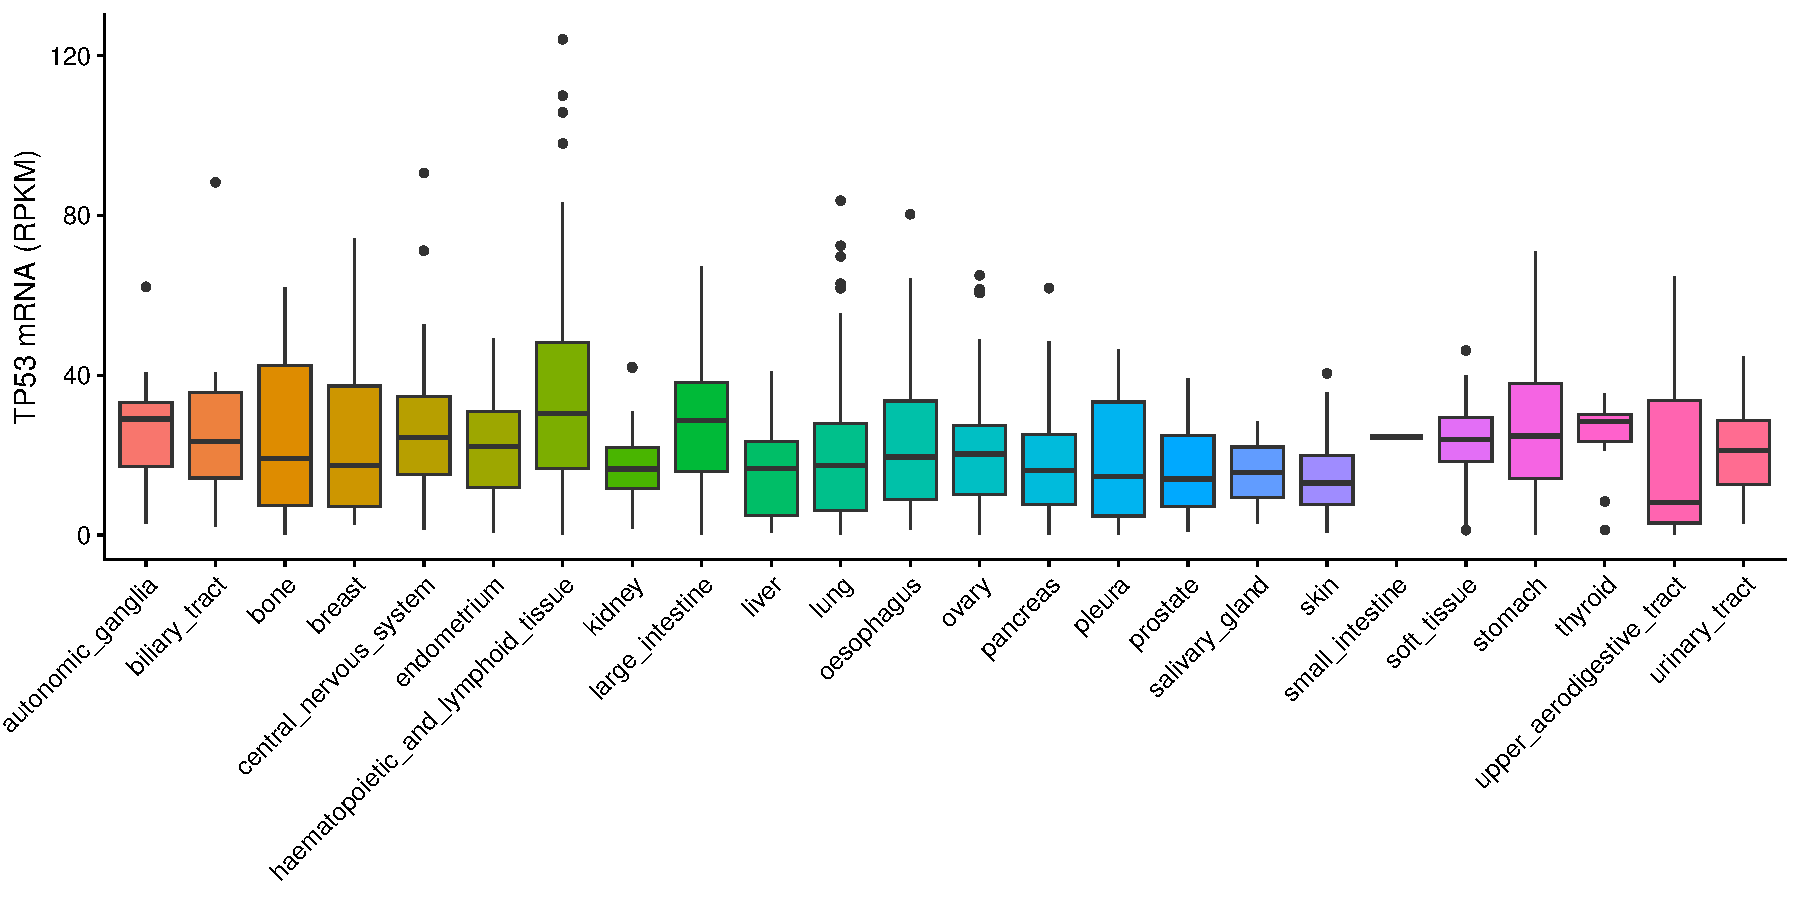
\includegraphics{_main_files/figure-latex/vis-ccle-tpm-1} \end{center}

\subsection{Correlation analysis}\label{correlation-analysis-2}

\subsubsection{\texorpdfstring{\href{https://openbiox.github.io/UCSCXenaShiny/reference/vis_ccle_gene_cor.html}{vis\_ccle\_gene\_cor()}}{vis\_ccle\_gene\_cor()}}\label{vis-ccle-gene-cor}

Calculate the correlation between two molecules value in one tissue type of cancer cell lines. (\hyperref[m-vis-ccle-gene-cor]{Custom module})

\begin{itemize}
\tightlist
\item
  Basic use: \texttt{vis\_ccle\_gene\_cor(Gene1=\ ,data\_type1=\ ,Gene2=\ ,data\_type2=\ ,SitePrimary=\ )}
\end{itemize}

\begin{Shaded}
\begin{Highlighting}[]
\FunctionTok{vis\_ccle\_gene\_cor}\NormalTok{(}\AttributeTok{Gene1 =} \StringTok{"CSF1R"}\NormalTok{, }\AttributeTok{data\_type1 =} \StringTok{"mRNA"}\NormalTok{, }
                  \AttributeTok{Gene2 =} \StringTok{"JAK3"}\NormalTok{, }\AttributeTok{data\_type2 =} \StringTok{"mRNA"}\NormalTok{, }
                  \AttributeTok{SitePrimary =} \StringTok{"prostate"}\NormalTok{)}
\end{Highlighting}
\end{Shaded}

\begin{center}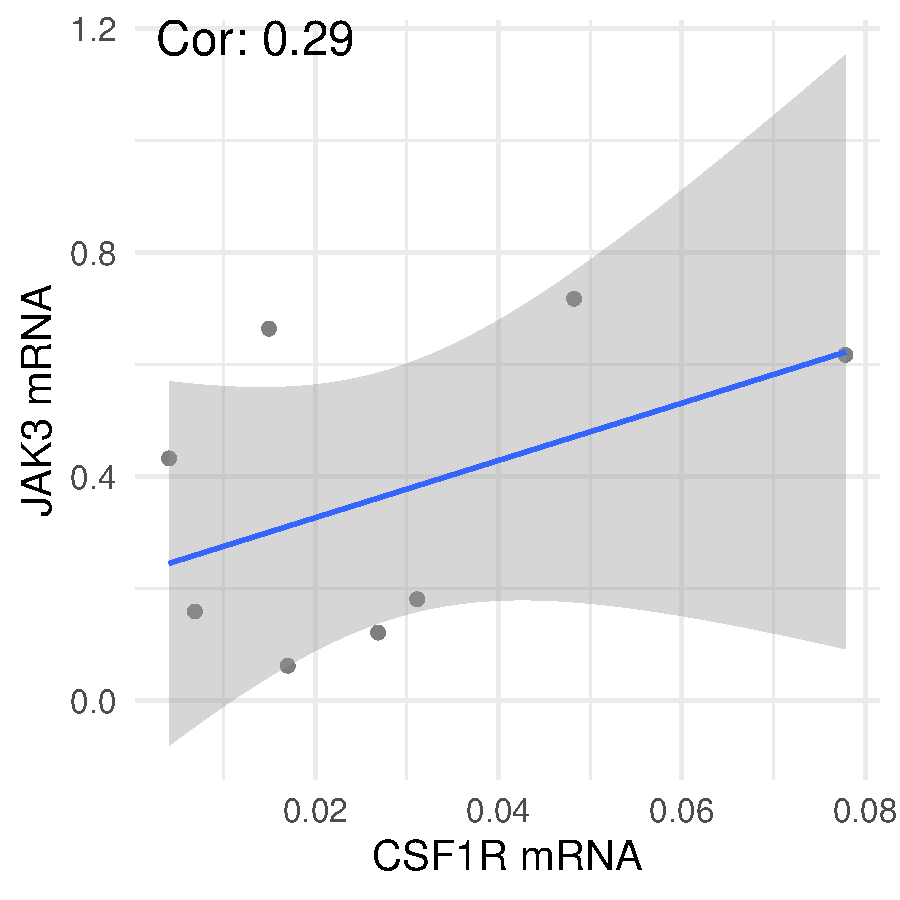
\includegraphics{_main_files/figure-latex/vis-ccle-gene_cor-1} \end{center}

\begin{quote}
\texttt{vis\_gene\_drug\_response\_diff()} and \texttt{vis\_gene\_drug\_response\_asso()} are initially designed for drug pharmacogenomics analysis. In the updated shiny application, we have provided more comprehensive pharmacogenomics analysis.
\end{quote}

\section{General analysis}\label{general-analysis}

\begin{table}

\caption{\label{tab:analyze-general-func}Specilized functions to analyze General molecular data}
\centering
\begin{tabular}[t]{lll}
\toprule
Database & Type & Function\\
\midrule
General & Comparison & vis\_identifier\_grp\_comparison()\\
General & Correlation & vis\_identifier\_cor()\\
General & Correlation & vis\_identifier\_multi\_cor()\\
General & Survival & vis\_identifier\_grp\_surv()\\
General & Dimension Reduction & vis\_identifier\_dim\_dist()\\
\bottomrule
\end{tabular}
\end{table}

\subsection{Comparison analysis}\label{comparison-analysis-1}

\subsubsection{\texorpdfstring{\href{https://openbiox.github.io/UCSCXenaShiny/reference/vis_identifier_grp_comparison.html}{vis\_identifier\_grp\_comparison()}}{vis\_identifier\_grp\_comparison()}}\label{vis-identifier-grp-comparison}

Compare molecular value between custom groups based on one genomics matrix UCSC Xena dataset. (\hyperref[m-vis-identifier-grp-comparison]{Custom module})

\begin{itemize}
\tightlist
\item
  Basic use: \texttt{vis\_identifier\_grp\_comparison(dataset=\ ,\ id=\ ,grp\_df=\ )}
\end{itemize}

\begin{Shaded}
\begin{Highlighting}[]
\CommentTok{\# Firstly, prepare custom groups of samples}
\FunctionTok{library}\NormalTok{(UCSCXenaTools)}
\NormalTok{cli\_df }\OtherTok{\textless{}{-}} \FunctionTok{XenaGenerate}\NormalTok{(}
  \AttributeTok{subset =}\NormalTok{ XenaDatasets }\SpecialCharTok{==} \StringTok{"TCGA.LUAD.sampleMap/LUAD\_clinicalMatrix"}
\NormalTok{) }\SpecialCharTok{\%\textgreater{}\%}
  \FunctionTok{XenaQuery}\NormalTok{() }\SpecialCharTok{\%\textgreater{}\%}
  \FunctionTok{XenaDownload}\NormalTok{() }\SpecialCharTok{\%\textgreater{}\%}
  \FunctionTok{XenaPrepare}\NormalTok{()}
\NormalTok{grp\_df }\OtherTok{=}\NormalTok{ cli\_df[, }\FunctionTok{c}\NormalTok{(}\StringTok{"sampleID"}\NormalTok{, }\StringTok{"pathologic\_M"}\NormalTok{)] }\SpecialCharTok{\%\textgreater{}\%}
\NormalTok{  dplyr}\SpecialCharTok{::}\FunctionTok{filter}\NormalTok{(pathologic\_M }\SpecialCharTok{\%in\%} \FunctionTok{c}\NormalTok{(}\StringTok{"M0"}\NormalTok{, }\StringTok{"M1"}\NormalTok{, }\StringTok{"MX"}\NormalTok{))}
\FunctionTok{head}\NormalTok{(grp\_df) }\CommentTok{\# col{-}1: sample; col{-}2: grouping info}
\end{Highlighting}
\end{Shaded}

\begin{verbatim}
## # A tibble: 6 x 2
##   sampleID        pathologic_M
##   <chr>           <chr>       
## 1 TCGA-05-4244-01 M1          
## 2 TCGA-05-4249-01 M0          
## 3 TCGA-05-4250-01 M0          
## 4 TCGA-05-4382-01 M0          
## 5 TCGA-05-4384-01 M0          
## 6 TCGA-05-4389-01 M0
\end{verbatim}

\begin{Shaded}
\begin{Highlighting}[]
\NormalTok{mol\_dataset }\OtherTok{\textless{}{-}} \StringTok{"TCGA.LUAD.sampleMap/HiSeqV2\_percentile"}
\FunctionTok{vis\_identifier\_grp\_comparison}\NormalTok{(}\AttributeTok{dataset =}\NormalTok{ mol\_dataset, }\AttributeTok{id =} \StringTok{"TP53"}\NormalTok{, }
                              \AttributeTok{grp\_df =}\NormalTok{ grp\_df)}
\end{Highlighting}
\end{Shaded}

\begin{center}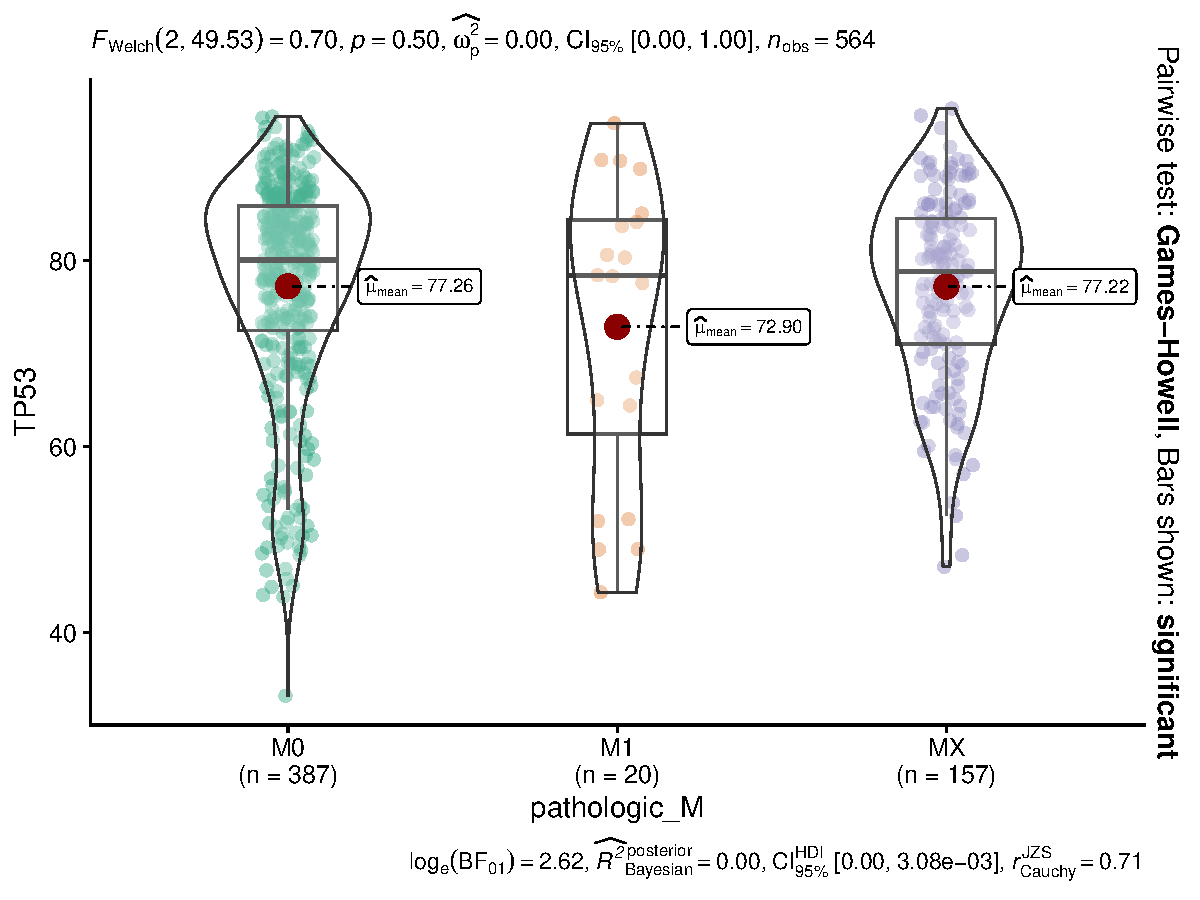
\includegraphics{_main_files/figure-latex/vis-identifier-grp-comparison-1} \end{center}

\subsection{Correlation analysis}\label{correlation-analysis-3}

\subsubsection{\texorpdfstring{\href{https://openbiox.github.io/UCSCXenaShiny/reference/vis_identifier_cor.html}{vis\_identifier\_cor()}}{vis\_identifier\_cor()}}\label{vis-identifier-cor}

Calculate the correlation between two molecules value from genomics matrix UCSC Xena datasets. (\hyperref[m-vis-identifier-cor]{Custom module})

\begin{itemize}
\tightlist
\item
  Basic use: \texttt{vis\_identifier\_cor(dataset=\ ,id1=\ ,dataset=\ ,id2=\ )}
\end{itemize}

\begin{Shaded}
\begin{Highlighting}[]
\NormalTok{dataset }\OtherTok{\textless{}{-}} \StringTok{"TcgaTargetGtex\_rsem\_isoform\_tpm"}
\FunctionTok{vis\_identifier\_cor}\NormalTok{(}\AttributeTok{dataset1 =}\NormalTok{ dataset, }\AttributeTok{id1 =} \StringTok{"TP53"}\NormalTok{,}
                   \AttributeTok{dataset2 =}\NormalTok{ dataset, }\AttributeTok{id2 =} \StringTok{"KRAS"}\NormalTok{)}
\end{Highlighting}
\end{Shaded}

\begin{verbatim}
## Warning: package 'ggpubr' was built under R version 4.4.3
\end{verbatim}

\begin{center}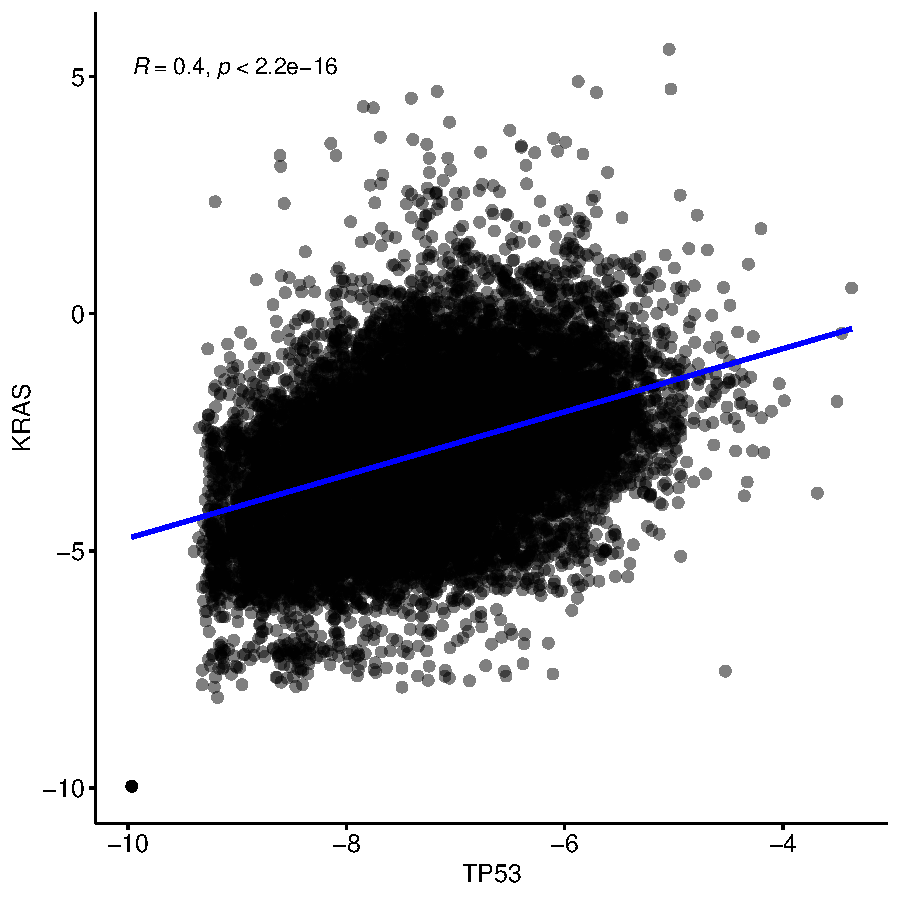
\includegraphics{_main_files/figure-latex/vis-identifier-cor-1} \end{center}

\subsubsection{\texorpdfstring{\href{https://openbiox.github.io/UCSCXenaShiny/reference/vis_identifier_multi_cor.html}{vis\_identifier\_multi\_cor()}}{vis\_identifier\_multi\_cor()}}\label{vis-identifier-multi-cor}

Calculate the pairwise correlation among multiple molecules value from one genomics matrix UCSC Xena dataset. (\hyperref[m-vis-identifier-multi-cor]{Custom module})

\begin{itemize}
\tightlist
\item
  Basic use: \texttt{vis\_identifier\_multi\_cor(dataset=\ ,ids=\ )}
\end{itemize}

\begin{Shaded}
\begin{Highlighting}[]
\NormalTok{dataset }\OtherTok{\textless{}{-}} \StringTok{"TcgaTargetGtex\_rsem\_isoform\_tpm"}
\FunctionTok{vis\_identifier\_multi\_cor}\NormalTok{(}\AttributeTok{dataset =}\NormalTok{ dataset,}
                         \AttributeTok{ids =} \FunctionTok{c}\NormalTok{(}\StringTok{"TP53"}\NormalTok{, }\StringTok{"KRAS"}\NormalTok{, }\StringTok{"PTEN"}\NormalTok{))}
\end{Highlighting}
\end{Shaded}

\begin{center}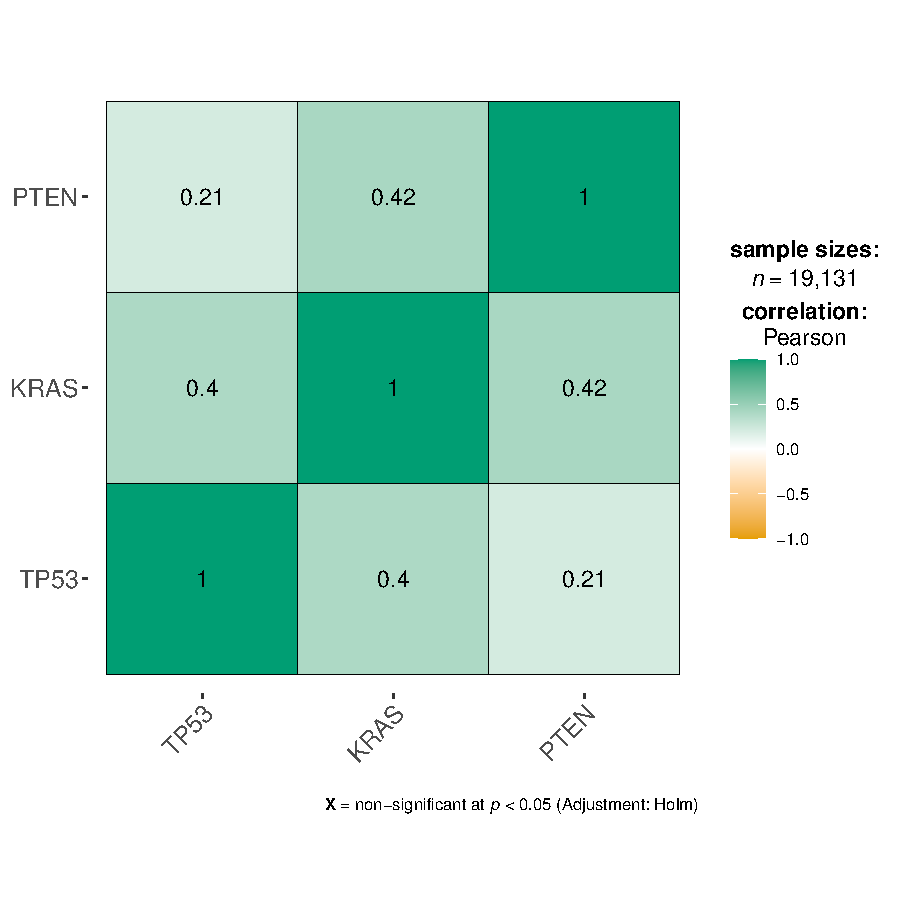
\includegraphics{_main_files/figure-latex/vis-identifier-multi-cor-1} \end{center}

\subsection{Survival analysis}\label{survival-analysis-2}

\subsubsection{\texorpdfstring{\href{https://openbiox.github.io/UCSCXenaShiny/reference/vis_identifier_grp_surv.html}{vis\_identifier\_grp\_surv()}}{vis\_identifier\_grp\_surv()}}\label{vis-identifier-grp-surv}

Perform the log-rank test of one molecule for one genomics matrix UCSC Xena dataset. (\hyperref[m-vis-identifier-grp-surv]{Custom module})

\begin{itemize}
\tightlist
\item
  Basic use: \texttt{vis\_identifier\_grp\_surv(dataset=\ ,\ id=\ ,\ surv\_df=\ )}
\end{itemize}

\begin{Shaded}
\begin{Highlighting}[]
\CommentTok{\# Firstly, prepare survival data of samples}
\FunctionTok{library}\NormalTok{(UCSCXenaTools)}
\NormalTok{cli\_df }\OtherTok{\textless{}{-}} \FunctionTok{XenaGenerate}\NormalTok{(}
  \AttributeTok{subset =}\NormalTok{ XenaDatasets }\SpecialCharTok{==} \StringTok{"TCGA.LUAD.sampleMap/LUAD\_clinicalMatrix"}
\NormalTok{) }\SpecialCharTok{\%\textgreater{}\%}
  \FunctionTok{XenaQuery}\NormalTok{() }\SpecialCharTok{\%\textgreater{}\%}
  \FunctionTok{XenaDownload}\NormalTok{() }\SpecialCharTok{\%\textgreater{}\%}
  \FunctionTok{XenaPrepare}\NormalTok{()}
\NormalTok{surv\_df }\OtherTok{\textless{}{-}}\NormalTok{ cli\_df[, }\FunctionTok{c}\NormalTok{(}\StringTok{"sampleID"}\NormalTok{, }\StringTok{"days\_to\_death"}\NormalTok{, }\StringTok{"vital\_status"}\NormalTok{)]}
\NormalTok{surv\_df}\SpecialCharTok{$}\NormalTok{vital\_status }\OtherTok{\textless{}{-}} \FunctionTok{ifelse}\NormalTok{(surv\_df}\SpecialCharTok{$}\NormalTok{vital\_status }\SpecialCharTok{==} \StringTok{"DECEASED"}\NormalTok{, }\DecValTok{1}\NormalTok{, }\DecValTok{0}\NormalTok{)}
\NormalTok{surv\_df }\OtherTok{=} \FunctionTok{na.omit}\NormalTok{(surv\_df)}
\FunctionTok{head}\NormalTok{(surv\_df)  }\CommentTok{\# col{-}1: sample; col{-}2: survival time; col{-}3: survival status}
\end{Highlighting}
\end{Shaded}

\begin{verbatim}
## # A tibble: 6 x 3
##   sampleID        days_to_death vital_status
##   <chr>                   <dbl>        <dbl>
## 1 TCGA-05-4250-01           121            1
## 2 TCGA-05-4395-01             0            1
## 3 TCGA-05-4396-01           303            1
## 4 TCGA-05-4397-01           731            1
## 5 TCGA-05-4402-01           244            1
## 6 TCGA-05-4415-01            91            1
\end{verbatim}

\begin{Shaded}
\begin{Highlighting}[]
\NormalTok{mol\_dataset }\OtherTok{\textless{}{-}} \StringTok{"TCGA.LUAD.sampleMap/HiSeqV2\_percentile"}
\FunctionTok{vis\_identifier\_grp\_surv}\NormalTok{(}\AttributeTok{dataset =}\NormalTok{ mol\_dataset, }\AttributeTok{id =} \StringTok{"KRAS"}\NormalTok{, }
                        \AttributeTok{surv\_df =}\NormalTok{ surv\_df)}
\end{Highlighting}
\end{Shaded}

\begin{figure}

{\centering 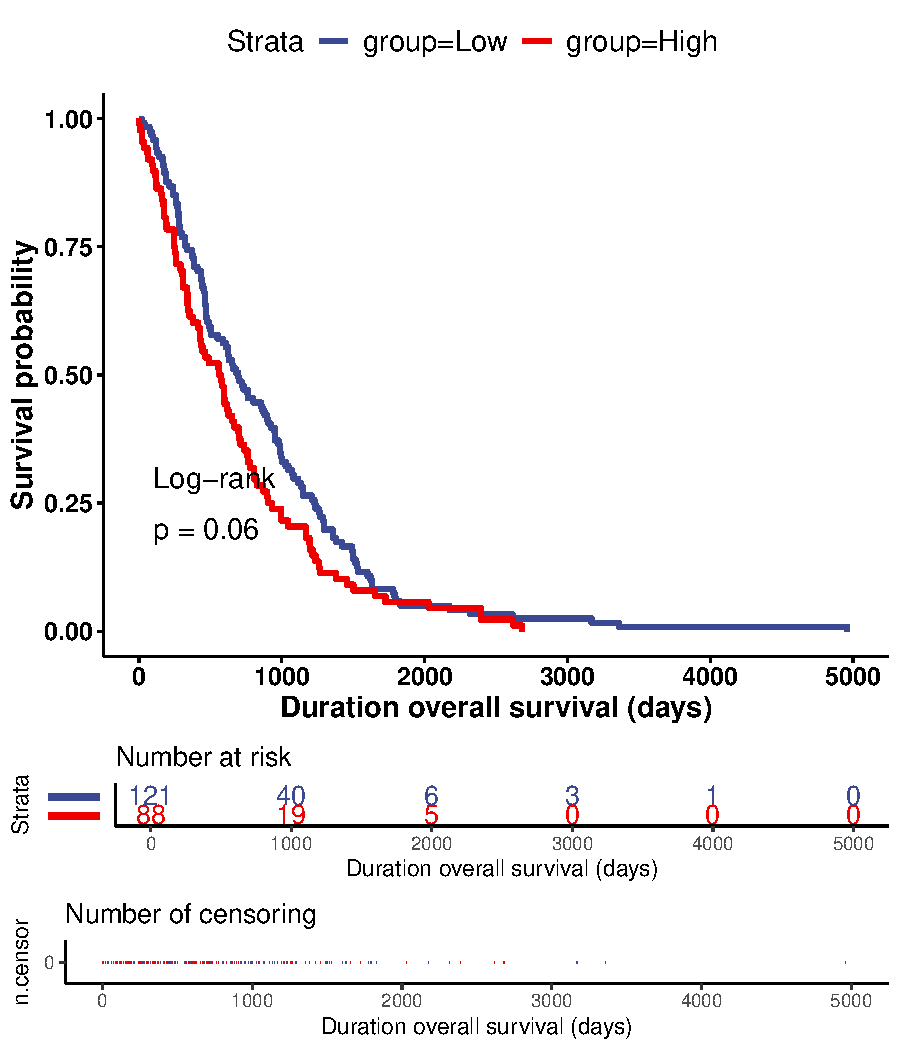
\includegraphics{_main_files/figure-latex/vis-identifier-grp-surv-1} 

}

\caption{The log-rank test (DSS) of mRNA KRAS for ne specific dataset}\label{fig:vis-identifier-grp-surv}
\end{figure}

\begin{quote}
By default, the best cutoff is decided. User can change it through the \texttt{cutoff\_mode} parameter.
\end{quote}

\subsection{Dimension reduction}\label{dimension-reduction-1}

\subsubsection{\texorpdfstring{\href{https://openbiox.github.io/UCSCXenaShiny/reference/vis_identifier_dim_dist.html}{vis\_identifier\_dim\_dist()}}{vis\_identifier\_dim\_dist()}}\label{vis-identifier-dim-dist}

Perform dimension reduction analysis of multiple molecules for samples in groups. (\hyperref[m-vis-identifier-dim-dist]{Custom module})

\begin{itemize}
\tightlist
\item
  Basic use: \texttt{vis\_identifier\_dim\_dist(dataset=\ ,ids=\ ,\ grp\_df=\ )}
\end{itemize}

\begin{Shaded}
\begin{Highlighting}[]
\CommentTok{\# Firstly, prepare the grouping information of samples }
\FunctionTok{library}\NormalTok{(UCSCXenaTools)}
\NormalTok{cli\_dataset }\OtherTok{\textless{}{-}} \StringTok{"TCGA.LUAD.sampleMap/LUAD\_clinicalMatrix"}
\NormalTok{cli\_df }\OtherTok{\textless{}{-}} \FunctionTok{XenaGenerate}\NormalTok{(}
  \AttributeTok{subset =}\NormalTok{ XenaDatasets }\SpecialCharTok{==}\NormalTok{ cli\_dataset}
\NormalTok{) }\SpecialCharTok{\%\textgreater{}\%}
  \FunctionTok{XenaQuery}\NormalTok{() }\SpecialCharTok{\%\textgreater{}\%}
  \FunctionTok{XenaDownload}\NormalTok{() }\SpecialCharTok{\%\textgreater{}\%}
  \FunctionTok{XenaPrepare}\NormalTok{()}
\NormalTok{grp\_df }\OtherTok{=}\NormalTok{ cli\_df[, }\FunctionTok{c}\NormalTok{(}\StringTok{"sampleID"}\NormalTok{, }\StringTok{"gender"}\NormalTok{)]}
\FunctionTok{head}\NormalTok{(grp\_df) }\CommentTok{\# col{-}1: sample; col{-}2: grouping info}
\end{Highlighting}
\end{Shaded}

\begin{verbatim}
## # A tibble: 6 x 2
##   sampleID        gender
##   <chr>           <chr> 
## 1 TCGA-05-4244-01 MALE  
## 2 TCGA-05-4249-01 MALE  
## 3 TCGA-05-4250-01 FEMALE
## 4 TCGA-05-4382-01 MALE  
## 5 TCGA-05-4384-01 MALE  
## 6 TCGA-05-4389-01 MALE
\end{verbatim}

\begin{Shaded}
\begin{Highlighting}[]
\NormalTok{mol\_dataset }\OtherTok{\textless{}{-}} \StringTok{"TCGA.LUAD.sampleMap/HiSeqV2\_percentile"}
\NormalTok{ids }\OtherTok{=} \FunctionTok{c}\NormalTok{(}\StringTok{"TP53"}\NormalTok{, }\StringTok{"KRAS"}\NormalTok{, }\StringTok{"PTEN"}\NormalTok{, }\StringTok{"MDM2"}\NormalTok{, }\StringTok{"CDKN1A"}\NormalTok{)}
\FunctionTok{vis\_identifier\_dim\_dist}\NormalTok{(}\AttributeTok{dataset =}\NormalTok{ mol\_dataset,}
                        \AttributeTok{ids =}\NormalTok{ ids, }
                        \AttributeTok{grp\_df =}\NormalTok{ grp\_df)}
\end{Highlighting}
\end{Shaded}

\begin{figure}

{\centering 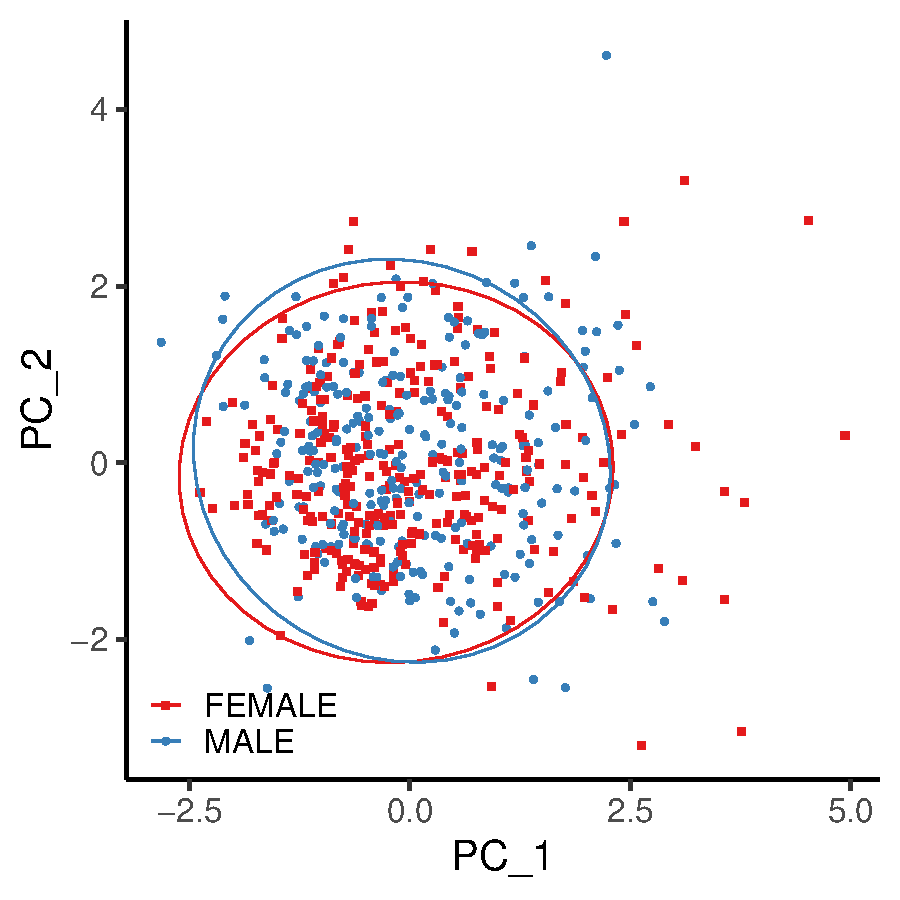
\includegraphics{_main_files/figure-latex/vis-identifier-dim-dist-1} 

}

\caption{The dimension reduction analysis (PCA) of 5 mRNA molcules in BRCA cancer samples grouped by tissue codes}\label{fig:vis-identifier-dim-dist}
\end{figure}

\part{Shiny App}\label{part-shiny-app}

\chapter{Visit}\label{visit}

\section{Server deployments}\label{server-deployments}

We have deployed the shiny application in two server machines for users without local installation.

\begin{itemize}
\tightlist
\item
  \url{http://shiny.zhoulab.ac.cn/UCSCXenaShiny}
\item
  \url{https://shiny.hiplot.cn/ucsc-xena-shiny}
\end{itemize}

\begin{figure}

{\centering \includegraphics[width=1\linewidth]{images/p0701} 

}

\caption{The welcome page of shiny application}\label{fig:p0701}
\end{figure}

\section{Local deployment}\label{local-deployment}

If the R package has been installed on your computer, it is easy to run the application in the local environment.

\begin{Shaded}
\begin{Highlighting}[]
\FunctionTok{app\_run}\NormalTok{()}
\end{Highlighting}
\end{Shaded}

Notably, the application is also dependent on some supplementary datasets (not in UCSC Xena) for extensive analysis. Considering the store limitation of R package and GitHub project, parts of them are deposited in \href{https://zenodo.org/record/10778172}{Zenodo repository}. When you first initiate the app, it could take some time to fetch these data. If it failed due to network, you can directly download them from Zenodo and then place on the \texttt{inst/extdata} directory.

\begin{figure}

{\centering \includegraphics[width=1\linewidth]{images/p0702} 

}

\caption{The supplementary data in the inst/extdata directory}\label{fig:p0702}
\end{figure}

\chapter{Homepage}\label{home}

\section{Quick Molecule Exploration}\label{quick-molecule-exploration}

In the top-right of homepage, two modules are provided for quick exploration of cancer molecules.

\begin{figure}

{\centering \includegraphics[width=1\linewidth]{images/p0804} 

}

\caption{Quick molecular exploration in the homepage}\label{fig:quick-explore}
\end{figure}

\subsection{Daily Gene}\label{daily-gene}

\begin{enumerate}
\def\labelenumi{\arabic{enumi}.}
\tightlist
\item
  In this module, a gene will be randomly selected each day and analyzed for which type of TCGA cancer is differentially expressed.
\item
  TPM expression data is obtained from TCGA and GTEx samples. For ease of presentation, the samples with minimum expression value of -9.966 are removed.
\item
  The wilcoxon test is used, and the cancer with the lowest P value will be displayed via \texttt{plotly} package.
\item
  Two external links to GeneCards and PubMed are also provided to search more information about the gene.
\item
  Finally, users can sample another gene to perform similar analysis if they want.
\end{enumerate}

\subsection{Pan-cancer Query}\label{pan-cancer-query}

In this module, two functions can be used to explore the pan-cancer features of one multi-omics molecule.

\subsubsection{Tumor vs.~Normal}\label{tumor-vs.-normal}

Observe and compare the molecular values in each TCGA project of normal tissue versus tumor tissue.

\begin{quote}
Tips: The analysis is based on \texttt{vis\_toil\_TvsN()} function referring to \ref{fig:vis-toil-TvsN}
\end{quote}

\begin{figure}

{\centering \includegraphics[width=1\linewidth]{images/p0806} 

}

\caption{The interface when clicking "Tumor vs. Normal" button}\label{fig:tumor-normal}
\end{figure}

\subsubsection{Generate Report}\label{generate-report}

\begin{enumerate}
\def\labelenumi{\arabic{enumi}.}
\tightlist
\item
  For general exploration of pan-cancer feature, a well-organized report report can be automatically generated.
\item
  As the following figure shows, it firstly run the analyses given the queried molecule, which will take about one minute. Then, you can knit the report in HTML format (figure) or directly download the analyzed results in ZIP format.
\end{enumerate}

\begin{figure}

{\centering \includegraphics[width=1\linewidth]{images/p0807} 

}

\caption{The interface when clicking "Generate Report" button and result}\label{fig:generate-report}
\end{figure}

\begin{enumerate}
\def\labelenumi{\arabic{enumi}.}
\setcounter{enumi}{2}
\tightlist
\item
  The report can be generally divided into five parts to describe molecular pan-cancer features, including (1) clinical phenotypes, (2) survival influence, (3) tumor index, (4) immune infiltration, (5) pathway activity.
  \textbackslash begin\{figure\}
\end{enumerate}

\{\centering \includegraphics[width=0.8\linewidth]{images/p0809}

\}

\caption{Five main parts of molecular report}

\label{fig:five-parts}
\textbackslash end\{figure\}

\begin{enumerate}
\def\labelenumi{\arabic{enumi}.}
\setcounter{enumi}{3}
\tightlist
\item
  Here is an \href{https://lishensuo.github.io/UCSCXenaShiny_Book/example_report.html}{example report} for mRNA TP53.
\end{enumerate}

\begin{figure}

{\centering \includegraphics[width=20.29in]{images/p0808} 

}

\caption{Head part of demo report}\label{fig:demo-report}
\end{figure}

\section{Slick Gallery}\label{slick-gallery}

\begin{itemize}
\tightlist
\item
  Dynamically display all application interfaces and their functional descriptions.
\end{itemize}

\begin{figure}

{\centering \includegraphics[width=1\linewidth]{images/p0801} 

}

\caption{Shiny Slick Gallery}\label{fig:slick-gallery}
\end{figure}

\section{TCGA Analysis Guide}\label{tcga-analysis-guide}

\begin{itemize}
\tightlist
\item
  Based on UCSC Xena datasets, we have designed versatile analyses for TCGA as well as other databases (PCAWG and CCLE).
\item
  In the homepage, examples of TCGA analyses, including 3 custom modules and 3 personalized pipelines, are displayed as quick interface for users.
\end{itemize}

\begin{figure}

{\centering \includegraphics[width=1\linewidth]{images/p0802} 

}

\caption{Example TCGA analysis}\label{fig:tcga-modules}
\end{figure}

\chapter{Repository}\label{repo}

Explore the metadata information of random UCSC Xena datasets in the repository page. Go to Chapter \ref{intro} if you have little knowledge about the UCSC Xena datasets.

\begin{enumerate}
\def\labelenumi{(\arabic{enumi})}
\item
  Firstly, users can query datasets according to the conditions of data hub (or further cohort) and data type (or further data subtype). By default, it will select the GDC hub and all data types.
\item
  Then, the basic information of eligible datasets will be display in the right panel.
\item
  Next, users can select one or multiple rows (datasets) and their external links to download or browse original data are available in the bottom.
\end{enumerate}

\begin{figure}

{\centering \includegraphics[width=1\linewidth]{images/p0901} 

}

\caption{Repoistory page demonstration}\label{fig:repo-page}
\end{figure}

\begin{enumerate}
\def\labelenumi{(\arabic{enumi})}
\setcounter{enumi}{3}
\tightlist
\item
  Furtherly, \textbf{three buttons} are designed for the selected datasets to offer specific functions as follows:
\end{enumerate}

\section{Show Metadata}\label{show-metadata}

\begin{itemize}
\tightlist
\item
  The ``Show Metadata'' button will give more detailed information of selected datasets.
\end{itemize}

\begin{figure}

{\centering \includegraphics[width=1\linewidth]{images/p0902} 

}

\caption{The interface when clicking "Show Metadata" button}\label{fig:show-meta}
\end{figure}

\section{Request Data}\label{request-data}

Through this button, three ways of downloading raw datasets are provided.

\begin{itemize}
\tightlist
\item
  ``Download data directly'': Enable to directly download the data into your local device.
\item
  ``Batch download in terminal'': Generate one \texttt{.sh} script file to download in Linux environment.
\item
  ``Copy R download code'': Generate R codes to download especially for R users.
\end{itemize}

\begin{figure}

{\centering \includegraphics[width=1\linewidth]{images/p0903} 

}

\caption{The interface when clicking "Request Data" button}\label{fig:requ-data}
\end{figure}

\section{Analyze Data}\label{analyze-data}

This button is the initial step for \textbf{General Dataset Analysis}, which will be introduced in Chapter \ref{general-da}.

\begin{itemize}
\tightlist
\item
  As the following figure shows, users need to firstly select one or more datasets in the repository page for the \texttt{Pre-selected\ Datasets\ for\ Analysis} panel in General Dataset Analysis page.
\item
  If one genomics matrix dataset (e.g.~RNA-seq) is selected, its related clinical metadata (e.g.~phenotype or survival data) will be automatically added.
\end{itemize}

\begin{figure}

{\centering \includegraphics[width=1\linewidth]{images/p0904} 

}

\caption{The initial step of General Dataset Analysis}\label{fig:anal-data}
\end{figure}

\chapter{General Analysis}\label{general-da}

\begin{enumerate}
\def\labelenumi{\arabic{enumi}.}
\tightlist
\item
  In this page, users can explore the most genomics matrix datasets of UCSC Xena repository with common analysis methods.
\item
  As Chapter \ref{analyze-data} describes, the initial step involves the selection of interesting datasets from \textbf{Repository} page.
\item
  In the following, we will take the ``\emph{TCGA-BLCA.htseq\_fpkm.tsv}'' dataset as an example to demonstrate how to perform various analyses.
\end{enumerate}

\begin{figure}

{\centering \includegraphics[width=1\linewidth]{images/p1001} 

}

\caption{The selection of TCGA-BLCA.htseq_fpkm.tsv dataset}\label{fig:p1001}
\end{figure}

\section{Scatter-Correlation}\label{m-vis-identifier-cor}

Compute and visualize the correlation between two molecules based on \hyperref[vis-identifier-cor]{\texttt{vis\_identifier\_cor()}} function.

\begin{enumerate}
\def\labelenumi{\arabic{enumi}.}
\tightlist
\item
  Firstly, select two molecules from candidate dataset(s);
\item
  Click the ``Submit'' button to perform analysis and the visualization result along with raw data will be display in the middle.
\item
  Finally, the plot can be saved with size and format options.
\end{enumerate}

\begin{figure}

{\centering \includegraphics[width=1\linewidth]{images/p1002} 

}

\caption{The steps of Scatter-Correlation analysis}\label{fig:p1002}
\end{figure}

\begin{quote}
Notably, two molecules can come from different datasets, but there must be intersecting samples.
\end{quote}

\section{Matrix-Correlation}\label{m-vis-identifier-multi-cor}

Compute and visualize the pair-wise correlation among multiple molecules based on \hyperref[vis-identifier-multi-cor]{\texttt{vis\_identifier\_multi\_cor()}} function.

\begin{enumerate}
\def\labelenumi{\arabic{enumi}.}
\tightlist
\item
  Firstly, select multiple molecules from one candidate dataset;
\item
  Modify several analysis and visualization parameters;
\item
  Click the ``Submit'' button to perform analysis and the visualization result along with analyzed data will be display in the middle.
\item
  Finally, the plot can be saved with size and format options.
\end{enumerate}

\begin{figure}

{\centering \includegraphics[width=1\linewidth]{images/p1003} 

}

\caption{The steps of Matrix-Correlation analysis}\label{fig:p1003}
\end{figure}

\section{Group-Comparison}\label{m-vis-identifier-grp-comparison}

Compare the differences in the distribution of values for one molecule under a specified phenotypic grouping based on \hyperref[vis-identifier-grp-comparison]{\texttt{vis\_identifier\_grp\_comparison()}} function.

\begin{enumerate}
\def\labelenumi{\arabic{enumi}.}
\tightlist
\item
  Select a dataset and use one of its columns as the basis for grouping. \textbf{(dataset 1)}
\item
  Select a dataset and use one of its numeric columns as the values to compare. \textbf{(dataset 2)}
\end{enumerate}

\begin{figure}

{\centering \includegraphics[width=1\linewidth]{images/p1004} 

}

\caption{The steps of Group-Comparison analysis}\label{fig:p1004}
\end{figure}

\begin{quote}
Based on above two selections, then set sample groups by clicking ``Preprocess'' button.

\begin{itemize}
\tightlist
\item
  Step1: From the columns of dataset 1, select the sample id column (\texttt{Sample\ column}), which is usually left as a default. Then, select a column (\texttt{Group\ column}) as the basis for grouping. If it is a numeric column, you can set the percentile cutoffs by the slider widget.
\item
  Step2: From the columns of dataset 2, select the sample id column (\texttt{Sample\ column}) and molecule column (\texttt{Value\ column}).
\item
  Step3: Click the ``Click to joint the data'' button to finally generate grouping result. If there are no problems, exit this interface.
\end{itemize}
\end{quote}

\begin{figure}

{\centering \includegraphics[width=1\linewidth]{images/p1005} 

}

\caption{The Group-Comparison grouping via the Preprocess button}\label{fig:p1005}
\end{figure}

\begin{enumerate}
\def\labelenumi{\arabic{enumi}.}
\setcounter{enumi}{2}
\tightlist
\item
  Modify several analysis parameters;
\item
  Click the ``Submit'' button to perform analysis and the visualization result along with raw data will be display in the middle.
\item
  Finally, the plot can be saved with size and format options.
\end{enumerate}

\section{Survival-Analysis}\label{m-vis-identifier-grp-surv}

Perform the grouping log-rank survival analysis, especially for TCGA related datasets based on \hyperref[vis-identifier-grp-surv]{\texttt{vis\_identifier\_grp\_surv()}} function.

\begin{enumerate}
\def\labelenumi{\arabic{enumi}.}
\tightlist
\item
  Select a dataset and use one of its columns as the basis for grouping. \textbf{(dataset 1)}
\item
  Select one survival dataset with event time and status columns. \textbf{(dataset 2)}
\end{enumerate}

\begin{figure}

{\centering \includegraphics[width=1\linewidth]{images/p1006} 

}

\caption{The steps of Survival-Analysis}\label{fig:p1006}
\end{figure}

\begin{quote}
Based on above two selections, then set sample groups by clicking ``Preprocess'' button.

\begin{itemize}
\tightlist
\item
  Step1: From the columns of dataset 1, select the sample id column (\texttt{Sample\ column}), which is usually left as a default. Then, select a column (\texttt{Group\ column}) as the basis for grouping. If it is a numeric column, you can set the percentile cutoffs by the slider widget or automatically calculate its best cutoff.
\item
  Step2: From the columns of dataset 2, select the sample id column (\texttt{Sample\ column}) and two survival related column (\texttt{Time\ column}, \texttt{Status\ column}).
\item
  Step3: Click the ``Click to joint the data'' button to finally generate grouping result. If there are no problems, exit this interface.
\end{itemize}
\end{quote}

\begin{figure}

{\centering \includegraphics[width=1\linewidth]{images/p1007} 

}

\caption{The Survival-Analysis grouping via the Preprocess button}\label{fig:p1007}
\end{figure}

\begin{enumerate}
\def\labelenumi{\arabic{enumi}.}
\setcounter{enumi}{2}
\tightlist
\item
  Click the ``Submit'' button to perform analysis and the visualization result along with raw data will be display in the middle.
\item
  Finally, the plot can be saved with size and format options.
\end{enumerate}

\section{Dimension-Distribution}\label{m-vis-identifier-dim-dist}

Perform the dimension reduction analysis based on multiple molecules of one genomics matrix datasets based on \hyperref[vis-identifier-dim-dist]{\texttt{vis\_identifier\_dim\_dist()}} function.

\begin{enumerate}
\def\labelenumi{\arabic{enumi}.}
\tightlist
\item
  Select a dataset and use one of its columns as the basis for grouping. \textbf{(dataset 1)}
\item
  Select a genomics matrix dataset and further multiple molecular columns via three ways. \textbf{(dataset 2)}.

  \begin{itemize}
  \tightlist
  \item
    ``Select'': One-by-one selection;
  \item
    ``Pathway'': batch selection under one pathway;
  \item
    ``File'': Upload of identifier file.
  \end{itemize}
\end{enumerate}

\begin{figure}

{\centering \includegraphics[width=1\linewidth]{images/p1008} 

}

\caption{The steps of Dimension-Distribution}\label{fig:p1008}
\end{figure}

\begin{quote}
Based on above two selections, then set sample groups by clicking ``Preprocess'' button.

\begin{itemize}
\tightlist
\item
  Step1: From the columns of dataset 1, select the sample id column (\texttt{Sample\ column}), which is usually left as a default. Then, select a column (\texttt{Group\ column}) as the basis for grouping. If it is a numeric column, you can set the percentile cutoffs by the slider widget.
\item
  Step2: From the columns of dataset 2, select the sample id column (\texttt{Sample\ column}) and molecule columns (\texttt{Value\ column}).
\item
  Step3: Click the ``Click to joint the data'' button to finally generate grouping result. If there are no problems, exit this interface.
\end{itemize}
\end{quote}

\begin{figure}

{\centering \includegraphics[width=1\linewidth]{images/p1009} 

}

\caption{The Dimension-Distribution grouping via the Preprocess button}\label{fig:p1009}
\end{figure}

\begin{enumerate}
\def\labelenumi{\arabic{enumi}.}
\setcounter{enumi}{2}
\tightlist
\item
  Modify several analysis and visualization parameters;

  \begin{itemize}
  \tightlist
  \item
    three DR methods (PCA/UMAP/TSNE) are supported.
  \end{itemize}
\item
  Click the ``Submit'' button to perform analysis and the visualization result along with analyzed data will be display in the middle.
\item
  Finally, the plot can be saved with size and format options.
\end{enumerate}

\chapter{TPC Modules}\label{custom-tpc}

In the ``Custom TPC modules'' page, there are totally 10 series of modules to quickly explore TPC (\textbf{T}CGA, \textbf{P}CAWG, \textbf{C}CLE) datasets with easy steps, based on the functions introduced in Chapter \ref{data-analysis}.

\begin{figure}

{\centering \includegraphics[width=0.8\linewidth]{images/p1101} 

}

\caption{All Custom TPC modules in shiny app}\label{fig:p1101}
\end{figure}

\section{TCGA}\label{tcga-1}

\begin{table}

\caption{\label{tab:custom-tcga-mod}Custom modules for TCGA analysis}
\centering
\begin{tabular}[t]{lll}
\toprule
Database & Type & Module\\
\midrule
TCGA & Comparison & Tumor VS Normal (Box plot)\\
TCGA & Comparison & Tumor VS Normal (Anatomy plot)\\
TCGA & Comparison & Mutation VS Wild\\
TCGA & Correlation & Molecule-Molecule\\
TCGA & Correlation & Molecule-Tumor Immune Infiltration\\
\addlinespace
TCGA & Correlation & Molecule-Immune Signature\\
TCGA & Correlation & Molecule-TMB/Stemness/MSI\\
TCGA & Correlation & Molecule-Pathway\\
TCGA & Survival & Kaplan-Meier\\
TCGA & Survival & Cox regression\\
\addlinespace
TCGA & Dimension Reduction & Dimension reduction\\
\bottomrule
\end{tabular}
\end{table}

\subsection{Comparison}\label{comparison}

\subsubsection{TCGA Tumor VS Normal (Box plot)}\label{tcga-tumor-vs-normal-box-plot}

Compare molecular values between tumor and normal samples combing TCGA and GTEx datasets based on \hyperref[vis-toil-TvsN]{\texttt{vis\_toil\_TvsN()}} and \hyperref[vis-toil-TvsN-cancer]{\texttt{vis\_toil\_TvsN\_cancer()}} functions.

\begin{itemize}
\tightlist
\item
  Left panel
\end{itemize}

\begin{enumerate}
\def\labelenumi{\arabic{enumi}.}
\tightlist
\item
  Select one of supported multi-omics types;
\item
  Select an identifier or define a signature;
\item
  Select the mode: Pan-cancer or Single-Cancer (For the latter, one tumor type needs to be specified);
\item
  Decide that Whether to include normal samples from GTEx;
\item
  Click the ``Go!'' button
\end{enumerate}

\begin{itemize}
\tightlist
\item
  Right panel
\end{itemize}

\begin{enumerate}
\def\labelenumi{\arabic{enumi}.}
\tightlist
\item
  Observe the visualization plot of analytical result;
\item
  Pull the sidebar to adjust plot parameters or download results through the top-right widget.
\end{enumerate}

\begin{figure}

{\centering \includegraphics[width=1\linewidth]{images/p1104} 

}

\caption{The layout of module "Tumor VS Normal (Box plot)"}\label{fig:p1104}
\end{figure}

\subsubsection{TCGA Tumor VS Normal (Anatomy plot)}\label{tcga-tumor-vs-normal-anatomy-plot}

Observe the difference of molecular values between pan-cancer tumor and normal samples based on \hyperref[vis-pancan-anatomy]{\texttt{vis\_pancan\_anatomy()}} functions.

\begin{itemize}
\tightlist
\item
  Left panel
\end{itemize}

\begin{enumerate}
\def\labelenumi{\arabic{enumi}.}
\tightlist
\item
  Select one of supported multi-omics types;
\item
  Select an identifier or define a signature;
\item
  Click the ``Go!'' button
\end{enumerate}

\begin{itemize}
\tightlist
\item
  Right panel
\end{itemize}

\begin{enumerate}
\def\labelenumi{\arabic{enumi}.}
\tightlist
\item
  Observe the anatomy plot of analytical result;
\item
  Pull the sidebar to adjust plot parameters or download results through the top-right widget.
\end{enumerate}

\begin{figure}

{\centering \includegraphics[width=1\linewidth]{images/p1104n} 

}

\caption{The layout of module "Tumor VS Normal (Anatomy plot)"}\label{fig:p1104n}
\end{figure}

\subsubsection{TCGA Mutation VS Wild}\label{m-vis-toil-Mut}

Compare molecular values between gene-mutant and gene-wild tumor samples based on \hyperref[vis-toil-Mut]{\texttt{vis\_toil\_Mut()}} and \hyperref[vis-toil-Mut-cancer]{\texttt{vis\_toil\_Mut\_cancer()}} functions.

\begin{itemize}
\tightlist
\item
  Left panel
\end{itemize}

\begin{enumerate}
\def\labelenumi{\arabic{enumi}.}
\tightlist
\item
  Select one of supported multi-omics types;
\item
  Select an identifier or define a signature to be compared;
\item
  Select one gene and group according to its mutation status;
\item
  Select the mode: Pan-cancer or Single-Cancer (For the latter, one tumor type needs to be specified);
\item
  Click the ``Go!'' button
\end{enumerate}

\begin{itemize}
\tightlist
\item
  Right panel
\end{itemize}

\begin{enumerate}
\def\labelenumi{\arabic{enumi}.}
\tightlist
\item
  Observe the visualization plot of analytical result;
\item
  Pull the sidebar to adjust plot parameters or download results through the top-right widget.
\end{enumerate}

\begin{figure}

{\centering \includegraphics[width=1\linewidth]{images/p1105} 

}

\caption{The steps of module "Mutation VS Wild"}\label{fig:p1105}
\end{figure}

\subsection{Correlation}\label{correlation}

\subsubsection{TCGA Molecule-Molecule}\label{m-vis-gene-cor}

Compute and visualize the correlation between two molecules of tumor samples based on \hyperref[vis-gene-cor]{\texttt{vis\_gene\_cor()}} and \hyperref[m-vis-gene-cor-cancer]{\texttt{vis\_gene\_cor\_cancer()}} functions.

\begin{itemize}
\tightlist
\item
  Left panel
\end{itemize}

\begin{enumerate}
\def\labelenumi{\arabic{enumi}.}
\tightlist
\item
  Select two respective omics types;
\item
  Select two specific identifiers as X-axis and Y-axis;
\item
  Select one or more TCGA types;
\item
  Select correlation method;
\item
  Decide that whether the correlation is corrected based on tumor purity;
\item
  Click the ``Go!'' button.
\end{enumerate}

\begin{itemize}
\tightlist
\item
  Right panel
\end{itemize}

\begin{enumerate}
\def\labelenumi{\arabic{enumi}.}
\tightlist
\item
  Observe the scatter plot of analytical result;
\item
  Pull the sidebar to adjust plot parameters or download results through the top-right widget.
\end{enumerate}

\begin{figure}

{\centering \includegraphics[width=1\linewidth]{images/p1106} 

}

\caption{The steps of module "Molecule-Molecule"}\label{fig:p1106}
\end{figure}

\subsubsection{TCGA Molecule-Tumor Immune Infiltration}\label{m-vis-gene-TIL-cor}

Compute the correlation of pan-cancers between one molecule and tumor immune infiltration of pan-cancer samples based on \hyperref[vis-gene-TIL-cor]{\texttt{vis\_gene\_TIL\_cor()}} function.

\begin{itemize}
\tightlist
\item
  Left panel
\end{itemize}

\begin{enumerate}
\def\labelenumi{\arabic{enumi}.}
\tightlist
\item
  Select one of supported multi-omics types;
\item
  Select an identifier or define a signature;
\item
  Select multiple TIL estimation;
\item
  Select correlation method;
\item
  Click the ``Go!'' button.
\end{enumerate}

\begin{itemize}
\tightlist
\item
  Right panel
\end{itemize}

\begin{enumerate}
\def\labelenumi{\arabic{enumi}.}
\tightlist
\item
  Observe the heatmap plot of analytical result;
\item
  Pull the sidebar to adjust plot parameters or download results through the top-right widget.
\end{enumerate}

\begin{figure}

{\centering \includegraphics[width=1\linewidth]{images/p1107} 

}

\caption{The steps of module "Molecule-Tumor Immune Infiltration"}\label{fig:p1107}
\end{figure}

\subsubsection{TCGA Molecule-Immune Signature}\label{m-vis-gene-immune-cor}

Compute the correlation of pan-cancers between one molecule and tumor Immune Signature based on \hyperref[vis-gene-immune-cor]{\texttt{vis\_gene\_immune\_cor()}} function.

\begin{itemize}
\tightlist
\item
  Left panel
\end{itemize}

\begin{enumerate}
\def\labelenumi{\arabic{enumi}.}
\tightlist
\item
  Select one of supported multi-omics types;
\item
  Select an identifier or define a signature;
\item
  Select one category of immune cell type scores;
\item
  Select correlation method;
\item
  Click the ``Go!'' button.
\end{enumerate}

\begin{itemize}
\tightlist
\item
  Right panel
\end{itemize}

\begin{enumerate}
\def\labelenumi{\arabic{enumi}.}
\tightlist
\item
  Observe the heatmap plot of analytical result;
\item
  Pull the sidebar to adjust plot parameters or download results through the top-right widget.
\end{enumerate}

\begin{figure}

{\centering \includegraphics[width=1\linewidth]{images/p1108} 

}

\caption{The steps of module "Molecule-Immune Signature"}\label{fig:p1108}
\end{figure}

\subsubsection{TCGA Molecule-TMB/Stemness/MSI}\label{m-vis-gene-index}

Compute the correlation of pan-cancers between one molecule and TMB/Stemness/MSI index based on \hyperref[vis-gene-tmb-cor]{\texttt{vis\_gene\_tmb\_cor()}}, \hyperref[vis-gene-msi-cor]{\texttt{vis\_gene\_msi\_cor()}} and \hyperref[vis-gene-stemness-cor]{\texttt{vis\_gene\_stemness\_cor()}} functions.

\begin{itemize}
\tightlist
\item
  Left panel
\end{itemize}

\begin{enumerate}
\def\labelenumi{\arabic{enumi}.}
\tightlist
\item
  Select one of supported multi-omics types;
\item
  Select an identifier or define a signature;
\item
  Select one of collected tumor index;
\item
  Select correlation method;
\item
  Click the ``Go!'' button.
\end{enumerate}

\begin{itemize}
\tightlist
\item
  Right panel
\end{itemize}

\begin{enumerate}
\def\labelenumi{\arabic{enumi}.}
\tightlist
\item
  Observe the radar plot of analytical result;
\item
  Pull the sidebar to adjust plot parameters or download results through the top-right widget.
\end{enumerate}

\begin{figure}

{\centering \includegraphics[width=1\linewidth]{images/p1109} 

}

\caption{The steps of module "Molecule-TMB/Stemness/MSI"}\label{fig:p1109}
\end{figure}

\subsubsection{TCGA Molecule-Pathway}\label{m-vis-gene-pw-cor}

Compute the correlation of between one molecule and pathway score of tumor samples based on \hyperref[vis-gene-pw-cor]{\texttt{vis\_gene\_pw\_cor()}} function.

\begin{itemize}
\tightlist
\item
  Left panel
\end{itemize}

\begin{enumerate}
\def\labelenumi{\arabic{enumi}.}
\tightlist
\item
  Select one of supported multi-omics types;
\item
  Select an identifier or define a signature;
\item
  Select one of calculated pathway scores (ssGSEA);
\item
  Select correlation method;
\item
  Click the ``Go!'' button.
\end{enumerate}

\begin{itemize}
\tightlist
\item
  Right panel
\end{itemize}

\begin{enumerate}
\def\labelenumi{\arabic{enumi}.}
\tightlist
\item
  Observe the scatter plot of analytical result;
\item
  Pull the sidebar to adjust plot parameters or download results through the top-right widget.
\end{enumerate}

\begin{figure}

{\centering \includegraphics[width=1\linewidth]{images/p1110} 

}

\caption{The steps of module "Molecule-Pathway"}\label{fig:p1110}
\end{figure}

\subsection{Survival analysis}\label{survival-analysis-3}

\subsubsection{TCGA Kaplan-Meier}\label{m-tcga-surv-plot}

Perform one molecular Log-rank survival analysis based on \hyperref[tcga-surv-plot]{\texttt{tcga\_surv\_plot()}} function.

\begin{itemize}
\tightlist
\item
  Left panel
\end{itemize}

\begin{enumerate}
\def\labelenumi{\arabic{enumi}.}
\tightlist
\item
  Select one of supported multi-omics types;
\item
  Select an identifier or define a signature;
\item
  Select one TCGA cancer and select one endpoint as survival event;
\item
  Filter samples by Gender, Age, Stage;
\item
  Select the grouping method;
\item
  Click the ``Go!'' button.
\end{enumerate}

\begin{itemize}
\tightlist
\item
  Right panel
\end{itemize}

\begin{enumerate}
\def\labelenumi{\arabic{enumi}.}
\tightlist
\item
  Observe the survival curves of analytical result;
\item
  Pull the sidebar to adjust plot parameters or download results through the top-right widget.
\end{enumerate}

\begin{figure}

{\centering \includegraphics[width=1\linewidth]{images/p1111} 

}

\caption{The steps of module "Kaplan-Meier"}\label{fig:p1111}
\end{figure}

\subsubsection{TCGA Cox regression}\label{m-vis-unicox-tree}

Perform one molecular Log-rank survival analysis across pan-cancers based on \hyperref[vis-unicox-tree]{\texttt{vis\_unicox\_tree()}} function.

\begin{itemize}
\tightlist
\item
  Left panel
\end{itemize}

\begin{enumerate}
\def\labelenumi{\arabic{enumi}.}
\tightlist
\item
  Select one of supported multi-omics types;
\item
  Select an identifier or define a signature;
\item
  Select one endpoint as survival event;
\item
  Click the ``Go!'' button.
\end{enumerate}

\begin{itemize}
\tightlist
\item
  Right panel
\end{itemize}

\begin{enumerate}
\def\labelenumi{\arabic{enumi}.}
\tightlist
\item
  Observe the forest plot of analytical result;
\item
  Pull the sidebar to adjust plot parameters or download results through the top-right widget.
\end{enumerate}

\begin{figure}

{\centering \includegraphics[width=1\linewidth]{images/p1112} 

}

\caption{The steps of module "Cox regression"}\label{fig:p1112}
\end{figure}

\subsection{Dimension Reduction}\label{dimension-reduction-2}

\subsubsection{TCGA Dimension reduction}\label{m-vis-dim-dist}

Perform molecular dimension reduction analysis based on \hyperref[vis-dim-dist]{\texttt{vis\_dim\_dist()}} function.

\begin{itemize}
\tightlist
\item
  Left panel
\end{itemize}

\begin{enumerate}
\def\labelenumi{\arabic{enumi}.}
\tightlist
\item
  Select one of supported multi-omics types;
\item
  Select multiple identifiers via one of three ways, then click the ``Cache data'' button;

  \begin{itemize}
  \tightlist
  \item
    ``Select'': One-by-one selection;
  \item
    ``Pathway'': batch selection under one pathway;
  \item
    ``File'': Upload of identifier file.
  \end{itemize}
\item
  Set the sample range and grouping;

  \begin{itemize}
  \tightlist
  \item
    ``Preset Group'': select one or more TCGA cancers and one clinical phenotype as grouping criteria.
  \item
    ``Custom Group'': upload files with custom samples and group columns. See details by downloading example file.
  \end{itemize}
\item
  Select the algorithm of dimension reduction;
\item
  Click the ``Go!'' button.
\end{enumerate}

\begin{itemize}
\tightlist
\item
  Right panel
\end{itemize}

\begin{enumerate}
\def\labelenumi{\arabic{enumi}.}
\tightlist
\item
  Observe the scatter plot of analytical result;
\item
  Pull the sidebar to adjust plot parameters or download results through the top-right widget.
\end{enumerate}

\begin{figure}

{\centering \includegraphics[width=1\linewidth]{images/p1113} 

}

\caption{The steps of module "Dimension reduction"}\label{fig:p1113}
\end{figure}

\section{PCAWG}\label{pcawg-1}

\begin{table}

\caption{\label{tab:custom-pcawg-mod}Custom modules for PCAWG analysis}
\centering
\begin{tabular}[t]{lll}
\toprule
Database & Type & Module\\
\midrule
PCAWG & Comparison & Tumor VS Normal\\
PCAWG & Correlation & Molecule-Molecule\\
PCAWG & Survival & Kaplan-Meier\\
PCAWG & Survival & Cox regression\\
\bottomrule
\end{tabular}
\end{table}

\subsection{Comparison analysis}\label{comparison-analysis-2}

\subsubsection{PCAWG Tumor VS Normal}\label{m-vis-pcawg-dist}

Compare molecular values between tumor and normal samples of PCAWG projects based on \hyperref[vis-pcawg-dist]{\texttt{vis\_pcawg\_dist()}} function.

\begin{itemize}
\tightlist
\item
  Left panel
\end{itemize}

\begin{enumerate}
\def\labelenumi{\arabic{enumi}.}
\tightlist
\item
  Select one of supported multi-omics types;
\item
  Select an identifier or define a signature;
\item
  Click the ``Go!'' button.
\end{enumerate}

\begin{itemize}
\tightlist
\item
  Right panel
\end{itemize}

\begin{enumerate}
\def\labelenumi{\arabic{enumi}.}
\tightlist
\item
  Observe the visualization plot of analytical result (Some of projects only have tumor samples);
\item
  Pull the sidebar to adjust plot parameters or download results through the top-right widget.
\end{enumerate}

\begin{figure}

{\centering \includegraphics[width=1\linewidth]{images/p1114} 

}

\caption{The steps of module "Tumor VS Normal"}\label{fig:p1114}
\end{figure}

\subsection{Correlation analysis}\label{correlation-analysis-4}

\subsubsection{PCAWG Molecule-Molecule}\label{m-vis-pcawg-gene-cor}

Compute and visualize the correlation between two molecules based on \hyperref[vis-pcawg-gene-cor]{\texttt{vis\_pcawg\_gene\_cor()}} function.

\begin{itemize}
\tightlist
\item
  Left panel
\end{itemize}

\begin{enumerate}
\def\labelenumi{\arabic{enumi}.}
\tightlist
\item
  Select two respective omics types;
\item
  Select two specific identifiers as X-axis and Y-axis;
\item
  Select one or more PCAWG projects;
\item
  Select correlation method;
\item
  Decide that whether the correlation is corrected based on tumor purity;
\item
  Click the ``Go!'' button.
\end{enumerate}

\begin{itemize}
\tightlist
\item
  Right panel
\end{itemize}

\begin{enumerate}
\def\labelenumi{\arabic{enumi}.}
\tightlist
\item
  Observe the scatter plot of analytical result;
\item
  Pull the sidebar to adjust plot parameters or download results through the top-right widget.
  \textbackslash begin\{figure\}
\end{enumerate}

\{\centering \includegraphics[width=1\linewidth]{images/p1115}

\}

\caption{The steps of module "Molecule-Molecule"}

\label{fig:p1115}
\textbackslash end\{figure\}

\subsection{Survival analysis}\label{survival-analysis-4}

\begin{quote}
Notes: Only OS endpoint for PCAWG samples.
\end{quote}

\subsubsection{PCAWG Kaplan-Meier}\label{pcawg-kaplan-meier}

Perform one molecular Log-rank survival analysis in one PCAWG project.

\begin{itemize}
\tightlist
\item
  Left panel
\end{itemize}

\begin{enumerate}
\def\labelenumi{\arabic{enumi}.}
\tightlist
\item
  Select one of supported multi-omics types;
\item
  Select an identifier or define a signature;
\item
  Select one PCAWG project;
\item
  Filter samples by Gender, Age;
\item
  Select the grouping method;
\item
  Click the ``Go!'' button.
\end{enumerate}

\begin{itemize}
\tightlist
\item
  Right panel
\end{itemize}

\begin{enumerate}
\def\labelenumi{\arabic{enumi}.}
\tightlist
\item
  Observe the survival curves of analytical result;
\item
  Pull the sidebar to adjust plot parameters or download results through the top-right widget.
\end{enumerate}

\begin{figure}

{\centering \includegraphics[width=1\linewidth]{images/p1116} 

}

\caption{The steps of module "Kaplan-Meier"}\label{fig:p1116}
\end{figure}

\subsubsection{PCAWG Cox regression}\label{m-vis-pcawg-unicox-tree}

Perform one molecular Log-rank survival analysis in All PCAWG projects based on \hyperref[vis-pcawg-unicox-tree]{\texttt{vis\_pcawg\_unicox\_tree()}} function.

\begin{itemize}
\tightlist
\item
  Left panel
\end{itemize}

\begin{enumerate}
\def\labelenumi{\arabic{enumi}.}
\tightlist
\item
  Select one of supported multi-omics types;
\item
  Select an identifier or define a signature;
\item
  Click the ``Go!'' button.
\end{enumerate}

\begin{itemize}
\tightlist
\item
  Right panel
\end{itemize}

\begin{enumerate}
\def\labelenumi{\arabic{enumi}.}
\tightlist
\item
  Observe the forest plot of analytical result;
\item
  Pull the sidebar to adjust plot parameters or download results through the top-right widget.
\end{enumerate}

\begin{figure}

{\centering \includegraphics[width=1\linewidth]{images/p1117} 

}

\caption{The steps of module "Cox regression"}\label{fig:p1117}
\end{figure}

\section{CCLE}\label{ccle-1}

\begin{table}

\caption{\label{tab:custom-ccle-mod}Custom modules for CCLE analysis}
\centering
\begin{tabular}[t]{lll}
\toprule
Database & Type & Module\\
\midrule
CCLE & Comparison & Cancer Primary Sites\\
CCLE & Correlation & Molecule-Molecule\\
\bottomrule
\end{tabular}
\end{table}

\subsection{Comparison analysis}\label{comparison-analysis-3}

\subsubsection{CCLE Cancer Primary Sites}\label{m-vis-ccle-tpm}

Compare molecular values of cancer cell lines from different primary site based on \hyperref[vis-ccle-tpm]{\texttt{vis\_ccle\_tpm()}} function.

\begin{itemize}
\tightlist
\item
  Left panel
\end{itemize}

\begin{enumerate}
\def\labelenumi{\arabic{enumi}.}
\tightlist
\item
  Select one of supported multi-omics types;
\item
  Select an identifier or define a signature;
\item
  Click the ``Go!'' button.
\end{enumerate}

\begin{itemize}
\tightlist
\item
  Right panel
\end{itemize}

\begin{enumerate}
\def\labelenumi{\arabic{enumi}.}
\tightlist
\item
  Observe the visualization plot of analytical result;
\item
  Pull the sidebar to adjust plot parameters or download results through the top-right widget.
\end{enumerate}

\begin{figure}

{\centering \includegraphics[width=1\linewidth]{images/p1118} 

}

\caption{The steps of module "Cancer Primary Sites"}\label{fig:p1118}
\end{figure}

\subsection{Correlation analysis}\label{correlation-analysis-5}

\subsubsection{CCLE Molecule-Molecule}\label{m-vis-ccle-gene-cor}

Compute and visualize the correlation between two molecules based on CCLE database based on \hyperref[vis-ccle-gene-cor]{\texttt{vis\_ccle\_gene\_cor()}} function.

\begin{itemize}
\tightlist
\item
  Left panel
\end{itemize}

\begin{enumerate}
\def\labelenumi{\arabic{enumi}.}
\tightlist
\item
  Select two respective omics types;
\item
  Select two specific identifiers as X-axis and Y-axis;
\item
  Select one or more primary sites;
\item
  Select correlation method;
\item
  Click the ``Go!'' button.
\end{enumerate}

\begin{itemize}
\tightlist
\item
  Right panel
\end{itemize}

\begin{enumerate}
\def\labelenumi{\arabic{enumi}.}
\tightlist
\item
  Observe the scatter plot of analytical result;
\item
  Pull the sidebar to adjust plot parameters or download results through the top-right widget.
\end{enumerate}

\begin{figure}

{\centering \includegraphics[width=1\linewidth]{images/p1119} 

}

\caption{The steps of module "Molecule-Molecule"}\label{fig:p1119}
\end{figure}

\chapter{TPC Pipelines(1)}\label{per-tpc-1}

\section{Extensive tumor data}\label{extensive-tumor-data}

\subsection{Compiling types of identifiers}\label{compiling-types-of-identifiers}

\begin{enumerate}
\def\labelenumi{\arabic{enumi}.}
\tightlist
\item
  For \textbf{TCGA} samples, there are \textbf{5} main data types and \textbf{23} subtypes (except for \emph{Custom metadata}).
\end{enumerate}

\begin{figure}

{\centering \includegraphics[width=1\linewidth]{images/p1201} 

}

\caption{Hierarchical types of TCGA Identifiers}\label{fig:p1201}
\end{figure}

\begin{enumerate}
\def\labelenumi{\arabic{enumi}.}
\setcounter{enumi}{1}
\item
  For \textbf{PCAWG} samples, there are \textbf{5} main data types and \textbf{17} subtypes (except for \emph{Custom metadata}).
\item
  For \textbf{CCLE} samples, there are \textbf{3} main data types and \textbf{6} subtypes (except for \emph{Custom metadata}).
\end{enumerate}

\begin{figure}

{\centering \includegraphics[width=1\linewidth]{images/p1202} 

}

\caption{Hierarchical types of PCAWG and CCLE Identifiers}\label{fig:p1202}
\end{figure}

About the core data type ------ \textbf{Molecular profile}, the initial step of all analysis pipelines involves the check and modification of molecular datasets through the \texttt{Modify\ datasets{[}opt{]}} widget. For some molecular types of TPC databases, there are alternative datasets for users to select, which greatly enriches the analytical possibilities

\begin{itemize}
\tightlist
\item
  Among the 7 types of TCGA molecules, 4 of them have the alternative datasets.
\end{itemize}

\begin{figure}

{\centering \includegraphics[width=1\linewidth]{images/p1102} 

}

\caption{Alternative datasets of TCGA molecules}\label{fig:p1102}
\end{figure}

\begin{quote}
Tips: For DNA Methylation, mean value of all CpG sites under one gene will be calculated for the gene by default. In the \texttt{Modify\ datasets{[}opt{]}} widget, users can furtherly limit its CpG sites and modify the aggregation method (e.g.~median).
\end{quote}

\begin{itemize}
\item
  Among the 5 types of PCAWG molecules, 2 of them have the alternative datasets.
\item
  Among the 4 types of CCLE molecules, 1 of them has the alternative datasets.
\end{itemize}

\begin{figure}

{\centering \includegraphics[width=1\linewidth]{images/p1103} 

}

\caption{Alternative datasets of PCAWG and CCLE molecules}\label{fig:p1103}
\end{figure}

\subsection{Reference of full identifiers}\label{reference-of-full-identifiers}

\begin{itemize}
\tightlist
\item
  In the ``\textbf{Help→ID query}'' page, all identifiers for ``\emph{Molecular profile}'', ``\emph{Tumor index}'', ``\emph{Immune Infiltration}'', ``\emph{Pathway activity}'', ``\emph{Phenotype data}'' types of TPC samples are compiling for easy query before analysis.
\item
  For example, valid identifiers under the \emph{TCGA mRNA Expression} subtype are shown in the following figure.
\end{itemize}

\begin{figure}

{\centering \includegraphics[width=1\linewidth]{images/p1203} 

}

\caption{TPC Identifiers Query Page}\label{fig:p1203}
\end{figure}

\subsection{User-defined identifiers}\label{user-defined-identifiers}

\subsubsection{Upload of random identifiers}\label{upload-of-random-identifiers}

\begin{enumerate}
\def\labelenumi{\arabic{enumi}.}
\tightlist
\item
  Users are enabled to upload random identifiers for joint analysis in the ``\textbf{Upload metadata}'' part of \textbf{S1} step.
\item
  The example file can be downloaded via the right button to see the format requirements.

  \begin{itemize}
  \tightlist
  \item
    .CSV file;
  \item
    The first column names ``Sample'' with sample ids (e.g.~``TCGA-OR-A5J1-01'' for TCGA samples). Only the intersected samples between this column and all TPC samples are considered;
  \item
    The other columns are random identifiers with continuous or categorical values.
  \end{itemize}
\item
  Upon successful identifiers upload, they will be added into the ``Custom metadata'' subtype of ``Phenotype data''.
\end{enumerate}

\begin{figure}

{\centering \includegraphics[width=0.8\linewidth]{images/p1204} 

}

\caption{Upload of random identifiers}\label{fig:p1204}
\end{figure}

\subsubsection{Design of custom signature}\label{design-of-custom-signature}

\begin{enumerate}
\def\labelenumi{\arabic{enumi}.}
\tightlist
\item
  Users can also design custom signature score based on self-defined molecular formula in the ``\textbf{Add signature}'' part of \textbf{S1} step.
\item
  Upon successful signature design and score calculation, they will also be added into the ``Custom metadata'' subtype of ``Phenotype data''.
\end{enumerate}

\begin{figure}

{\centering \includegraphics[width=0.8\linewidth]{images/p1205} 

}

\caption{Design of custom signature}\label{fig:p1205}
\end{figure}

\begin{enumerate}
\def\labelenumi{\arabic{enumi}.}
\setcounter{enumi}{2}
\tightlist
\item
  As shown in the figure below, the signature can be set as following steps after clicking Edit button.
\end{enumerate}

\begin{itemize}
\tightlist
\item
  Firstly, modify the name and select the molecular type;
\item
  Then, design the molecular formula comprised of multiple molecules with respective coefficients;

  \begin{itemize}
  \tightlist
  \item
    The coefficient of each molecule is divided into two parts (Directions and Absolute Coef).
  \item
    The ``\textbf{Del}'' button will cancel the last set molecule and the ``\textbf{Reset}'' button will undo all selected molecules.
  \item
    The real-time formula is shown in the bottom.
  \end{itemize}
\item
  Finally, click the ``Query data'' button to calculate the signature scores and click the right button to add the signature into the ``Custom metadata'' subtype of ``Phenotype data''. In addition, user can obtain the result locally via the bottom button.
\end{itemize}

\begin{figure}

{\centering \includegraphics[width=1\linewidth]{images/p1206} 

}

\caption{3 steps of signature design}\label{fig:p1206}
\end{figure}

\section{Sample processing}\label{sample-processing}

\begin{figure}

{\centering \includegraphics[width=0.8\linewidth]{images/p1207} 

}

\caption{Sample filtering and grouping modules}\label{fig:p1207}
\end{figure}

\subsection{Sample filtering}\label{sample-filtering}

After selecting one tumor, all its samples will be selected by default. Here, we provide two methods to obtain specific subpopulation in the ``\textbf{Filter samples}'' part of \textbf{S1} step.

\begin{figure}

{\centering \includegraphics[width=0.8\linewidth]{images/p1208} 

}

\caption{Sample filtering module}\label{fig:p1208}
\end{figure}

\subsubsection{Quick filter}\label{quick-filter}

Users can directly make quick selections based on tissue code (pathological) types of samples. Based on the \href{https://gdc.cancer.gov/resources-tcga-users/tcga-code-tables/sample-type-codes}{14th to 15th characters} of the TCGA sample ID (e.g., TCGA-19-1787-01), samples can be categorized into different types. The common code types involved in UCSCXenaShiny analysis are shown in the following table.

\begin{longtable}[]{@{}
  >{\raggedright\arraybackslash}p{(\linewidth - 4\tabcolsep) * \real{0.0588}}
  >{\raggedright\arraybackslash}p{(\linewidth - 4\tabcolsep) * \real{0.6912}}
  >{\raggedright\arraybackslash}p{(\linewidth - 4\tabcolsep) * \real{0.2500}}@{}}
\toprule\noalign{}
\begin{minipage}[b]{\linewidth}\raggedright
Code
\end{minipage} & \begin{minipage}[b]{\linewidth}\raggedright
Definition
\end{minipage} & \begin{minipage}[b]{\linewidth}\raggedright
Short Letter Code
\end{minipage} \\
\midrule\noalign{}
\endhead
\bottomrule\noalign{}
\endlastfoot
01 & Primary Solid Tumor & TP \\
02 & Recurrent Solid Tumor & TR \\
03 & Primary Blood Derived Cancer - Peripheral Blood & TB \\
05 & Additional - New Primary & TAP \\
06 & Metastatic & TM \\
07 & Additional Metastatic & TAM \\
11 & Solid Tissue Normal & NT \\
\end{longtable}

\begin{quote}
For PCAWG database, you can perform similar operation to quickly select tumor or normal samples. For CCLE database, there is no quick filter.
\end{quote}

\subsubsection{Exact filter}\label{exact-filter}

Through this module, users are enabled to perform personalized sample filtering. This followings are operational steps:

\begin{enumerate}
\def\labelenumi{\arabic{enumi}.}
\tightlist
\item
  Set the candidate conditions from comprehensive identifiers. Each addition will rename the selected identifier as ``Condition\_Num''.

  \begin{itemize}
  \tightlist
  \item
    When selecting molecular identifier as condition, it may take some time to download from the USCS Xena, depending on the network.
  \item
    For TPC samples, some basic clinical variables have been selected into the candidate pool. For TCGA samples, they include \emph{Age, Code, Gender, Stage\_ajcc, Stage\_clinical, Grade}.
  \end{itemize}
\item
  Get an overview of the distribution of each candidate condition for clear filtering .

  \begin{itemize}
  \tightlist
  \item
    For continuous variables, the mean and the distribution of multiple percentiles are displayed.
  \item
    For categorical variables, the frequency of each category is displayed.
  \end{itemize}
\item
  Perform filtering operation based on one or multiple conditions from the above candidate list. Total 6 operators are devised for versatile filtering give the type of each condition.

  \begin{itemize}
  \tightlist
  \item
    For categorical variable, ``\textbf{+}'' and ``\textbf{-}'' are used for retain or discard specific categories of samples.
  \item
    For continuous variable, ``\textbf{\textgreater{}}'' and ``\textbf{\textless{}}'' are used to set absolute cutoff, while ``\textbf{\%\textgreater{}}'' and ``\textbf{\%\textless{}}'' are used to set percentile cutoff.
  \end{itemize}
\end{enumerate}

\begin{figure}

{\centering \includegraphics[width=1\linewidth]{images/p1209} 

}

\caption{3 steps of sample filtering}\label{fig:p1209}
\end{figure}

\begin{quote}
Tips: If the percentile cutoff is involved, the results may vary based on the order of filtering, as illustrated in the example above figure.

\begin{itemize}
\tightlist
\item
  The first instance: Samples with the top 50\% high expression of TP53 in female samples. → \textbf{23} samples
\item
  The second instance: Females from the top 50\% of samples with high TP53 expression. → \textbf{28} samples
\end{itemize}
\end{quote}

\subsection{Sample grouping}\label{sample-grouping}

For binary comparison or survival analysis, it is necessary to divide the samples into two groups based on one specific condition. Here, we also provide a personalized grouping module to flexibly set two ranges of sample populations.

Generally, it has the two main steps:

\begin{enumerate}
\def\labelenumi{\arabic{enumi}.}
\item
  Select one condition and observe its distribution. Similar to the filtering module, it can bring a clear pre-knowledge by observing the distribution of one continuous or categorical condition.
\item
  Set two non-overlapping sample ranges to group.
\end{enumerate}

\begin{itemize}
\tightlist
\item
  For categorical variable, assign one or more classifications for both groups (\textbf{Left figure})
\item
  For continuous variable, set the minimum and max thresholds for both group.

  \begin{itemize}
  \tightlist
  \item
    By default, the first group (Group1) has lower value with \textbf{left close} and \textbf{right open} range, e.g.~{[}0, 1). If its left range is blank, it will represent the minimum value of the condition.
  \item
    And, the second group (Group2) has larger value with \textbf{left close} and \textbf{right close} range, e.g.~{[}0, 1{]}. If its right range is blank, it will represent the maximum value of the condition.
  \item
    The thresholds can be percentile values (\textbf{Middle figure}) or absolute values (\textbf{Right figure}) depending on purposes.
  \end{itemize}
\end{itemize}

\begin{figure}

{\centering \includegraphics[width=1\linewidth]{images/p1210} 

}

\caption{Sample grouping module}\label{fig:p1210}
\end{figure}

\begin{quote}
Tips: By default, the Group1 has the prior order during analysis and visualization. You can click the switch ``Whether reverse levels'' to change the order.
\end{quote}

\section{Data fetch}\label{data-fetch}

After sample selection and processing, we usually need to fetch data for downstream analysis.

\subsection{Single data}\label{single-data}

Most of time, we just need to select one identifier and fetch its values. According to the hierarchical organization (\textbf{Data type → Data subtype → Identifier}), select one interesting identifier and then click the ``Query button'' to fetch data. It's worth noting that, for \emph{Molecular profile} data types, it may take some time to download from the UCSC Xena, depending on the network.

\begin{figure}

{\centering \includegraphics[width=0.8\linewidth]{images/p1211} 

}

\caption{Fetch single data}\label{fig:p1211}
\end{figure}

\subsection{Multiple data}\label{multiple-data}

For batch analysis, we can select multiple identifiers based on one of three ways.

\begin{enumerate}
\def\labelenumi{\arabic{enumi}.}
\tightlist
\item
  In the first way (\textbf{Left figure}), user can select batch identifiers of one specific subtype one by one.
\item
  In the second way (\textbf{Middle figure}), user can select all identifiers of one specific subtype. Notably, for some molecular types with much identifiers, all the identifiers (gene/transcript) belong to one MSigDB signature can be selected.
\end{enumerate}

\begin{itemize}
\tightlist
\item
  These molecular types are ``mRNA Expression'', ``DNA Methylation'', ``Mutation status'', ``Copy Number Variation'', ``Transcript Expression''.
\item
  The MSigDB gene signatures are obtained via \href{https://igordot.github.io/msigdbr/}{\texttt{msigdbr} package}, which can be 9 main categories (bottom table).
\item
  Two links are available for detailed information of selected signature and MSigDB database.
\end{itemize}

\begin{enumerate}
\def\labelenumi{\arabic{enumi}.}
\setcounter{enumi}{2}
\tightlist
\item
  In the third way (\textbf{Right figure}), user can directly upload an identifier file with following requirements:
\end{enumerate}

\begin{itemize}
\tightlist
\item
  TXT format;
\item
  One column without colname;
\item
  Only the valid identifiers that overlapped with the selected data subtype are retained
\end{itemize}

\begin{figure}

{\centering \includegraphics[width=1\linewidth]{images/p1212} 

}

\caption{Fetch multiple data}\label{fig:p1212}
\end{figure}

\begin{center}\rule{0.5\linewidth}{0.5pt}\end{center}

\begin{longtable}[]{@{}
  >{\centering\arraybackslash}p{(\linewidth - 4\tabcolsep) * \real{0.0808}}
  >{\centering\arraybackslash}p{(\linewidth - 4\tabcolsep) * \real{0.3131}}
  >{\raggedright\arraybackslash}p{(\linewidth - 4\tabcolsep) * \real{0.6061}}@{}}
\toprule\noalign{}
\begin{minipage}[b]{\linewidth}\centering
Category
\end{minipage} & \begin{minipage}[b]{\linewidth}\centering
Notes
\end{minipage} & \begin{minipage}[b]{\linewidth}\raggedright
Subcategory
\end{minipage} \\
\midrule\noalign{}
\endhead
\bottomrule\noalign{}
\endlastfoot
H & hallmark gene sets & / \\
C1 & positional gene sets & / \\
C2 & curated gene sets & CGP, CP, CP:BIOCARTA, CP:KEGG, CP:PID, CP:REACTOME, CP:WIKIPATHWAYS \\
C3 & regulatory target gene sets & MIR:MIRDB, MIR:MIR\_Legacy, TFT:GTRD, TFT:TFT\_Legacy \\
C4 & computational gene sets & CGN, CM \\
C5 & ontology gene sets & \url{GO:BP}, \url{GO:CC}, \url{GO:MF}, HPO \\
C6 & oncogenic signature gene sets & / \\
C7 & immunologic signature gene sets & IMMUNESIGDB, VAX \\
C8 & cell type signature gene sets & / \\
\end{longtable}

\chapter{TPC Pipelines(2)}\label{per-tpc-2}

\section{General steps}\label{general-steps}

\textbf{S1: Preset} --- Set personalized samples and tumor data with following general steps.

\begin{itemize}
\tightlist
\item
  ``\textbf{Modify datasets}'': View the dataset sources for each molecular type. When there are alternative datasets for the same molecular type, users can switch a suitable one based on purpose (referring to Chapter \ref{custom-tpc}).
\item
  ``\textbf{Choose cancer}'': Choose one cancer type for downstream association analysis.
\item
  ``\textbf{Filter samples}'': Upon the selection of one tumor, further refine the samples based on tissue codes or personalized filtering module.
\item
  ``\textbf{Upload metadata}'': Upload user-defined tumor data for joint analysis.
\item
  ``\textbf{Add signature}'': Design custom molecular signature for joint analysis.
\end{itemize}

\textbf{S2: Get data} --- Select and fetch identifier values; set grouping information.

\textbf{S3: Analyze \& Visualize} --- Modify diverse parameters; perform analysis; download results.

\begin{itemize}
\tightlist
\item
  ``\textbf{Set analyzation parameters}'': Select different statistical methods
\item
  ``\textbf{Set visualization parameters}'': Adjust plot color, title text, etc.
\item
  ``\textbf{Download results}'': Download three types of results, including raw data, detailed statistical results and plot results. (Note: No plot for batch-screen mode).
\end{itemize}

\begin{quote}
Notes: We will introduce various analysis scenarios of TPC using TCGA as example.
\end{quote}

\section{Correlation analysis}\label{correlation-analysis-6}

\begin{figure}

{\centering \includegraphics[width=1\linewidth]{images/p1301} 

}

\caption{3 modes of correlation analysis}\label{fig:p1301}
\end{figure}

\subsection{Individual Mode}\label{individual-mode}

Perform the correlation analysis between any \textbf{two identifiers} of samples from \textbf{one tumor}.

The following is a simple example. (The steps not mentioned in above figure imply default operations.)

\textbf{S1: Preset}

\begin{itemize}
\tightlist
\item
  ``\textbf{S1.2 Choose cancer}'': choose the \textbf{\emph{CHOL}} (Cholangiocarcinoma) cancer type
\item
  ``\textbf{S1.3 Filter samples}'': choose the \textbf{\emph{primary tumor}} samples via the quick filter.
\end{itemize}

\textbf{S2: Get data}

\begin{itemize}
\tightlist
\item
  ``\textbf{S2.1 Get data for X-axis}'': Molecular profile→mRNA Expression→\textbf{\emph{TP53}}
\item
  ``\textbf{S2.2 Get data for Y-axis}'': Infiltration→CIBERSORT→ \textbf{\emph{Monocyte}}
\end{itemize}

\textbf{S3: Analyze \& Visualize}

\begin{itemize}
\tightlist
\item
  ``\textbf{S3.1 Set analysis parameters}'': \textbf{\emph{Spearman}}
\item
  ``\textbf{S3.2 Set visualization parameters}'': Adjust the main title name.
\end{itemize}

\begin{figure}

{\centering \includegraphics[width=1\linewidth]{images/p1302} 

}

\caption{Example of correlation analysis in individual mode}\label{fig:p1302}
\end{figure}

\subsection{Pan-cancer Mode}\label{pan-cancer-mode}

Perform the correlation analysis between any \textbf{two identifiers} of samples across \textbf{multiple tumors}.

The following is a simple example. (The steps not mentioned in above figure imply default operations.)

\textbf{S1: Preset}

\begin{itemize}
\tightlist
\item
  ``\textbf{S1.1 Modify datasets}'': Select the \textbf{Norm\_Count} dataset for mRNA Expression dataset.
\item
  ``\textbf{S1.2 Choose cancer}'': choose all TCGA cancer types.
\item
  ``\textbf{S1.3 Filter samples}'': choose the \textbf{\emph{non-normal}} samples via the quick filter.
\end{itemize}

\textbf{S2: Get data}

\begin{itemize}
\tightlist
\item
  ``\textbf{S2.1 Get data for X-axis}'': Molecular profile→mRNA Expression→\textbf{\emph{HDAC1}}
\item
  ``\textbf{S2.2 Get data for Y-axis}'': Molecular profile→mRNA Expression→\textbf{\emph{APOE}}
\end{itemize}

\textbf{S3: Analyze \& Visualize}

\begin{itemize}
\tightlist
\item
  ``\textbf{S3.1 Set analysis parameters}'': \textbf{\emph{Pearson}}
\item
  ``\textbf{S3.2 Set visualization parameters}'': Adjust the names of main title and axis title.
\end{itemize}

\begin{figure}

{\centering \includegraphics[width=1\linewidth]{images/p1303} 

}

\caption{Example of correlation analysis in pan-cancer mode}\label{fig:p1303}
\end{figure}

\subsection{Batch Screen Mode}\label{batch-screen-mode}

Perform the correlation analysis between \textbf{multiple identifiers} and \textbf{one identifier} of samples from \textbf{one tumor}.

The following is a simple example. (The steps not mentioned in above figure imply default operations.)

\textbf{S1: Preset}

\begin{itemize}
\tightlist
\item
  ``\textbf{S1.2 Choose cancer}'': choose the \textbf{\emph{CHOL}} (Cholangiocarcinoma) cancer type
\item
  ``\textbf{S1.3 Filter samples}'': choose the \textbf{\emph{primary tumor}} samples via the quick filter.
\end{itemize}

\textbf{S2: Get data}

\begin{itemize}
\tightlist
\item
  ``\textbf{S2.1 Get batch data for X-axis}'': Molecular profile→mRNA Expression→ genes of HALLMARK\_APOPTOSIS pathways
\item
  ``\textbf{S2.2 Get data for Y-axis}'': Immune Infiltration→CIBERSORT→ \textbf{\emph{Monocyte}}
\end{itemize}

\textbf{S3: Analyze}

\begin{itemize}
\tightlist
\item
  ``\textbf{S3.1 Set analysis parameters}'': \textbf{\emph{Spearman}}
\end{itemize}

\begin{figure}

{\centering \includegraphics[width=1\linewidth]{images/p1304} 

}

\caption{Example of correlation analysis in batch screen mode}\label{fig:p1304}
\end{figure}

\section{Comparison analysis}\label{comparison-analysis-4}

\begin{figure}

{\centering \includegraphics[width=1\linewidth]{images/p1305} 

}

\caption{3 modes of comparison analysis}\label{fig:p1305}
\end{figure}

\subsection{Individual Mode}\label{individual-mode-1}

Perform the comparison analysis of \textbf{one identifier} between two groups of samples from \textbf{one tumor}.

The following is a simple example. (The steps not mentioned in above figure imply default operations.)

\textbf{S1: Preset}

\begin{itemize}
\tightlist
\item
  ``\textbf{S1.2 Choose cancer}'': choose the \textbf{\emph{BRCA}} (Breast invasive carcinoma) cancer type
\item
  ``\textbf{S1.3 Filter samples}'': choose the \textbf{\emph{non-normal}} samples via the quick filter.
\end{itemize}

\textbf{S2: Get data}

\begin{itemize}
\tightlist
\item
  ``\textbf{S2.1 Divide 2 groups by one condition}'': Group1→\textbf{Primary} tumor samples; Group2→\textbf{Metastatic} tumor samples
\item
  ``\textbf{S2.2 Get data for comparison}'': Molecular profile→mRNA Expression→\textbf{\emph{POSTN}}
\end{itemize}

\textbf{S3: Analyze \& Visualize}

\begin{itemize}
\tightlist
\item
  ``\textbf{S3.1 Set analysis parameters}'': \textbf{\emph{Wilcoxon test}}
\item
  ``\textbf{S3.2 Set visualization parameters}'': Remove x-axis title.
\end{itemize}

\begin{figure}

{\centering \includegraphics[width=1\linewidth]{images/p1306} 

}

\caption{Example of comparison analysis in individual mode}\label{fig:p1306}
\end{figure}

\subsection{Pan-cancer Mode}\label{pan-cancer-mode-1}

Perform the comparison analysis of \textbf{one identifier} between two groups of samples across \textbf{multiple tumors}.

The following is a simple example. (The steps not mentioned in above figure imply default operations.)

\textbf{S1: Preset}

\begin{itemize}
\tightlist
\item
  ``\textbf{S1.2 Choose cancer}'': choose the all TCGA cancer types.
\item
  ``\textbf{S1.3 Filter samples}'': choose the \textbf{\emph{primary tumor}} samples via the quick filter. Further choose samples with age above 60 via the exact filter.
\end{itemize}

\textbf{S2: Get data}

\begin{itemize}
\tightlist
\item
  ``\textbf{S2.1 Divide 2 groups by one condition}'': Group1→ gene PTEN mutation; Group2→ gene PTEN wild-type.
\item
  ``\textbf{S2.2 Get data for comparison}'': Tumor index → Tumor Stemness →\textbf{\emph{RNAss}}
\end{itemize}

\textbf{S3: Analyze \& Visualize}

\begin{itemize}
\tightlist
\item
  ``\textbf{S3.1 Set analysis parameters}'': \textbf{\emph{t-test}}
\item
  ``\textbf{S3.2 Set visualization parameters}'': adjust x-axis title.
\end{itemize}

\begin{figure}

{\centering \includegraphics[width=1\linewidth]{images/p1307} 

}

\caption{Example of comparison analysis in pan-cancer mode}\label{fig:p1307}
\end{figure}

\subsection{Batch Screen Mode}\label{batch-screen-mode-1}

Perform the comparison analysis of \textbf{multiple identifier} between two groups of samples from \textbf{one tumor}.

The following is a simple example. (The steps not mentioned in above figure imply default operations.)

\textbf{S1: Preset}

\begin{itemize}
\tightlist
\item
  ``\textbf{S1.2 Choose cancer}'': choose the \textbf{\emph{BRCA}} (Breast invasive carcinoma) cancer type
\item
  ``\textbf{S1.3 Filter samples}'': choose the \textbf{\emph{non-normal}} samples via the quick filter.
\end{itemize}

\textbf{S2: Get data}

\begin{itemize}
\tightlist
\item
  ``\textbf{S2.1 Divide 2 groups by one condition}'': Group1→\textbf{Primary} tumor samples; Group2→\textbf{Metastatic} tumor samples
\item
  ``\textbf{S2.2 Get data for comparison}'': Immune Infiltration→XCELL→ \textbf{\emph{Monocyte}}
\end{itemize}

\textbf{S3: Analyze}

\begin{itemize}
\tightlist
\item
  ``\textbf{S3.1 Set analysis parameters}'': \textbf{\emph{Wilcoxon test}}
\end{itemize}

\begin{figure}

{\centering \includegraphics[width=1\linewidth]{images/p1308} 

}

\caption{Example of comparison analysis in batch screen mode}\label{fig:p1308}
\end{figure}

\section{Survival analysis}\label{survival-analysis-5}

By default, both log-rank and cox regression survival analysis are performed for two groups of samples divided according to one condition. Here, we devised a switch ``\textbf{\emph{Whether use initial data before grouping?}}'' at \textbf{S3.1} steps with following function:

\begin{itemize}
\item
  If its status is off , the above default analysis will performed;
\item
  If its status is on and the grouping condition is \textbf{continuous}:

  \begin{itemize}
  \tightlist
  \item
    For log-rank test, it will search the \textbf{optimal cutoff} with most significant survival difference;
  \item
    For Cox regression, it will directly build the cox model based on the continuous variable.
  \end{itemize}
\end{itemize}

\begin{figure}

{\centering \includegraphics[width=1\linewidth]{images/p1309} 

}

\caption{3 modes of survival analysis}\label{fig:p1309}
\end{figure}

\subsection{Individual Mode}\label{individual-mode-2}

Perform the survival analysis between two groups of samples generated by \textbf{one identifier} from \textbf{one tumor}.

The following is a simple example. (The steps not mentioned in above figure imply default operations.)

\textbf{S1: Preset}

\begin{itemize}
\tightlist
\item
  ``\textbf{S1.1 Modify datasets}'': Select the 27K Methylation datasets; Select the cg15206330 site to represent TP53 methylation
\item
  ``\textbf{S1.2 Choose cancer}'': choose the \textbf{\emph{BRCA}} (Breast invasive carcinoma) cancer type
\item
  ``\textbf{S1.3 Filter samples}'': choose the \textbf{\emph{non-normal}} samples via the quick filter.
\end{itemize}

\textbf{S2: Get data}

\begin{itemize}
\tightlist
\item
  ``\textbf{S2.1 Select survival endpoint}'': Select the OS event
\item
  ``\textbf{S2.2 Divide 2 groups by one condition}'': Group1: TP53 methylation higher 50\%, Group2: TP53 methylation lower 50\%
\end{itemize}

\textbf{S3: Analyze \& Visualize}

\begin{itemize}
\tightlist
\item
  ``\textbf{S3.1 Set analysis parameters}'': Log-rank text
\item
  ``\textbf{S3.2 Set visualization parameters}'': Modify color; Set confidence interval.
\end{itemize}

\begin{figure}

{\centering \includegraphics[width=1\linewidth]{images/p1310} 

}

\caption{Example of survival analysis in individual mode}\label{fig:p1310}
\end{figure}

\subsection{Pan-cancer Mode}\label{pan-cancer-mode-2}

Perform the survival analysis between two groups of samples generated by \textbf{one identifier} across \textbf{multiple tumor}.

The following is a simple example. (The steps not mentioned in above figure imply default operations.)

\textbf{S1: Preset}

\begin{itemize}
\tightlist
\item
  ``\textbf{S1.2 Choose cancer}'': choose the \textbf{\emph{BRCA}} cancer type
\item
  ``\textbf{S1.3 Filter samples}'': choose the \textbf{\emph{non-normal}} samples via the quick filter.
\end{itemize}

\textbf{S2: Get data}

\begin{itemize}
\tightlist
\item
  ``\textbf{S2.1 Select survival endpoint}'': Select the OS event
\item
  ``\textbf{S2.2 Divide 2 groups by one condition}'': Group1: Signature value higher 10\%, Group2: Signature value lower 10\%
\end{itemize}

\textbf{S3: Analyze \& Visualize}

\begin{itemize}
\tightlist
\item
  ``\textbf{S3.1 Set analysis parameters}'': Univariate Cox regression; Use the initial data.
\item
  ``\textbf{S3.2 Set visualization parameters}'': Add main title.
\end{itemize}

\begin{figure}

{\centering \includegraphics[width=1\linewidth]{images/p1311} 

}

\caption{Example of survival analysis in pan-cancer mode}\label{fig:p1311}
\end{figure}

\subsection{Batch Screen Mode}\label{batch-screen-mode-2}

Perform the survival analysis between two groups of samples generated by \textbf{multiple identifiers} from \textbf{one tumor}.

The following is a simple example. (The steps not mentioned in above figure imply default operations.)

\textbf{S1: Preset}

\begin{itemize}
\tightlist
\item
  ``\textbf{S1.2 Choose cancer}'': choose the all TCGA cancer types
\item
  ``\textbf{S1.3 Filter samples}'': choose the \textbf{\emph{primary tumor}} samples via the quick filter.
\item
  ``\textbf{S1.5 Add signature}'': Design a molecular signature and add to custom metadata.
\end{itemize}

\textbf{S2: Get data}

\begin{itemize}
\tightlist
\item
  ``\textbf{S2.1 Select survival endpoint}'': Select the PFI event
\item
  ``\textbf{S2.2 Divide 2 groups by one condition}'': Pathway activity→HALLMARK pathways→Group1: score higher 50\%, Group2: score lower 50\%
\end{itemize}

\textbf{S3: Analyze}

\begin{itemize}
\tightlist
\item
  ``\textbf{S3.1 Set analysis parameters}'': Log-rank test
\end{itemize}

\begin{figure}

{\centering \includegraphics[width=1\linewidth]{images/p1312} 

}

\caption{Example of survival analysis in batch screen mode}\label{fig:p1312}
\end{figure}

\section{Cross-Omics analysis}\label{cross-omics-analysis}

Recently, we have added one pipeline for TCGA cross-omics analysis to simultaneously explore the molecular features of multiple omics across pan-cancers.

\subsection{Gene Cross-Omics Analysis}\label{gene-cross-omics-analysis}

Perform the cross-omics analysis at the gene level, involving Gene expression, Gene Mutation, Gene CNV, Transcript expression, DNA methylation.

The following is a simple example. (The steps not mentioned in above figure imply default operations.)

\textbf{S1: Preset}

\begin{itemize}
\tightlist
\item
  ``\textbf{S1.2 Choose cancer}'': choose the all TCGA cancer types
\item
  ``\textbf{S1.3 Filter samples}'': By default, select all normal samples and tumor samples.
\end{itemize}

\textbf{S2: Get data}

\begin{itemize}
\tightlist
\item
  ``\textbf{S2.1 Select one gene}'': Select gene TP53
\item
  ``\textbf{S2.2 Load mRNA/Mutation/CNV data}'': Preload the mRNA/Mutation/CNV data of gene to save time in S3 step.
\item
  ``\textbf{S2.3 Load transcript data}'': Select and load several transcript of gene, filter invalid transcripts with null value.
\item
  ``\textbf{S2.4 Load methylation data}'': Select several CpG sits of gene and load methyaltion data.
\end{itemize}

\textbf{S3: Analyze \& Visualize} : Analyze multi-omics data and visualize by \texttt{funkyheatmap} package.

\begin{figure}

{\centering \includegraphics[width=1\linewidth]{images/p1313} 

}

\caption{Example of Gene Cross-Omics Analysis}\label{fig:p1313}
\end{figure}

\textbf{Column-1}: TCGA Names;

\textbf{Column-2{[}Expression Profile{]}}: 0-1 normalized median expression of gene in normal samples (include GTEx);

\textbf{Column-3{[}Expression Profile{]}}: 0-1 normalized median expression of gene in tumor samples;

\textbf{Column-4{[}Expression Profile{]}}: The significance symbol of gene comparison between tumor and normal samples via \emph{Wilcoxon} test (P\textless0.001, ``***''; P\textless0.01, ``**''; P\textless0.05, ``*''; P\textgreater0.05, ``-'').

\textbf{Column-5{[}Mutation Profile{]}}: The distribution of gene mutation or wild status in tumor samples.

\textbf{Column-6{[}Mutation Profile{]}}: The percentage of gene mutation status in tumor samples.

\textbf{Column-7{[}CNV Profile{]}}: The distribution of gene copy number variation status in tumor samples (-2, homozygous deletion; -1, single copy deletion; 0, diploid normal copy; 1: low-level copy number amplification; 2: high-level copy number amplification).

\textbf{Column-8{[}CNV Profile{]}}: The percentage of gene copy number amplification (1,2) in tumor samples.

\textbf{Column-9{[}CNV Profile{]}}: The percentage of gene copy number deletion (-1, -2) in tumor samples.

\textbf{Column-Selected transcript(s) of one gene{[}CNV Profile{]}}: The median transcript expression in tumor samples.

\textbf{Column-Selected CpG sites of one gene{[}Methylation Profile{]}}: The median beta value of CpG sites in tumor samples.

\subsection{Pathway Cross-Omics Analysis}\label{pathway-cross-omics-analysis}

Perform the cross-omics analysis at the pathway level, involving Gene expression, Gene Mutation, Gene CNV.

The following is a simple example. (The steps not mentioned in above figure imply default operations.)

\textbf{S1: Preset}

\begin{itemize}
\tightlist
\item
  ``\textbf{S1.2 Choose cancer}'': choose the all TCGA cancer types
\item
  ``\textbf{S1.3 Filter samples}'': By default, select all normal samples and tumor samples.
\end{itemize}

\textbf{S2: Get data}

\begin{itemize}
\tightlist
\item
  ``\textbf{S2.1 one pathway}'': Select pathway HALLMARK\_ADIPOGENESIS
\end{itemize}

\textbf{S3: Analyze \& Visualize} : Analyze multi-omics data and visualize by \texttt{funkyheatmap} package.

\begin{figure}

{\centering \includegraphics[width=1\linewidth]{images/p1314} 

}

\caption{Example of Pathway Cross-Omics Analysis}\label{fig:p1314}
\end{figure}

\textbf{Column-1}: TCGA Names;

\textbf{Column-2{[}Expression Profile{]}}: 0-1 normalized median ssGSEA score of pathway in normal samples (include GTEx);

\textbf{Column-3{[}Expression Profile{]}}: 0-1 normalized median ssGSEA score of gene in tumor samples;

\textbf{Column-4{[}Expression Profile{]}}: The significance symbol of gene comparison between tumor and normal samples via \emph{Wilcoxon} test (P\textless0.001, ``***''; P\textless0.01, ``**''; P\textless0.05, ``*''; P\textgreater0.05, ``-'').

\textbf{Column-5{[}Mutation Profile{]}}: The distribution of mutation or wild pathway gene status in tumor samples. If one of pathway genes is mutated, it is considered as mutation.

\textbf{Column-6{[}Mutation Profile{]}}: The percentage of pathway mutation status in tumor samples.

\textbf{Column-7{[}Mutation Profile{]}}: The mean counts of mutated pathway genes in tumor samples.

\textbf{Column-8{[}CNV Profile{]}}: The distribution of pathway gene copy number variation status in tumor samples. (Amp, homozygous deletion or single copy deletion; Non, diploid normal copy; Del, Copy number amplification.)

\textbf{Column-9{[}CNV Profile{]}}: The copy number amplification percentage of pathway genes in tumor samples.

\textbf{Column-10{[}CNV Profile{]}}: The copy number deletion percentage of pathway gene in tumor samples.

\chapter{Download Modules}\label{download}

Although the full datasets of UCSC Xena can be downloaded in the repository page, it will spend unnecessary time and storage costs if we only want to obtain several molecular data for local analysis.

Therefore, two download modules are designed for the precise acquisition of raw data from TCGA/PCAWG/CCLE analysis (module 1) and UCSC Xena repository datasets (module 2).

\begin{itemize}
\tightlist
\item
  If you want to quickly query and obtain omics values of TPC samples, the module 1 is more suitable. In addition, non-omics annotation data of TPC is also available (e.g.~tumor immune infiltration estimation).
\item
  If you want to search one specific UCSC Xena dataset, especially for other hubs (e.g.~TCGA GDC), the module 2 is more suitable.
\end{itemize}

\begin{figure}

{\centering \includegraphics[width=1\linewidth]{images/p1401} 

}

\caption{Two custom download modules}\label{fig:p1401}
\end{figure}

\section{Download TPC datasets}\label{download-tpc-datasets}

There are two parts for omics (Left) and non-omics (Right) data, respectively.

\subsection{Omics molecular data}\label{omics-molecular-data}

Go to Chapter \ref{intro} if you have little knowledge about the UCSC Xena datasets.

\begin{enumerate}
\def\labelenumi{\arabic{enumi}.}
\tightlist
\item
  Select one database and set the candidate datasets (referring to Chapter \ref{custom-tpc});
\item
  Select further samples through the quick or exact filters (referring to Chapter \ref{sample-filtering});
\item
  Select one specific molecular type and its multiple identifiers in three ways (referring to Chapter \ref{multiple-data});
\item
  Click the ``Query'' button to fetch the eligible data and display in the right panel;
\item
  Download the queried data into local CSV or RDA file.
\end{enumerate}

\begin{figure}

{\centering \includegraphics[width=1\linewidth]{images/p1402} 

}

\caption{The steps of TPC omics molecular data fetch}\label{fig:p1402}
\end{figure}

\subsection{Non-omics annotation data}\label{non-omics-annotation-data}

\begin{itemize}
\tightlist
\item
  For each of TPC databases, there are various non-omics annotation data for extensive molecular analysis;
\item
  In the most right panel, users can easily download one specific data via corresponding buttons;
\end{itemize}

\begin{figure}

{\centering \includegraphics[width=1\linewidth]{images/p1403} 

}

\caption{TPC non-omics annotation data}\label{fig:p1403}
\end{figure}

\section{Download UCSC Xena datasets}\label{download-ucsc-xena-datasets}

Go to Chapter \ref{intro} if you have little knowledge about the UCSC Xena datasets.

\begin{enumerate}
\def\labelenumi{\arabic{enumi}.}
\tightlist
\item
  Select one data hub in UCSC Xena;
\item
  Select one of candidate datasets by limiting the data format type and profile type;
\item
  Load all available identifiers of the selected dataset. The Primary ID indicates the row names of dataset and the ProbeMap ID is more usable. For instance, among most mRNA dataset, their Primary IDs are usually \emph{Ensembl} names and ProbeMap IDs are \emph{Symbol} names;
\item
  Select multiple identifiers or directly upload an id file;
\item
  Click the ``Query'' button to fetch the eligible data and display in the right panel;
\item
  Download the queried data into local CSV or RDA file.
\end{enumerate}

\begin{figure}

{\centering \includegraphics[width=1\linewidth]{images/p1404} 

}

\caption{The steps of UCSC Xena dataset fetch}\label{fig:p1404}
\end{figure}

  \bibliography{book.bib,packages.bib}

\end{document}
